%!TEX root = ../template.tex
%%%%%%%%%%%%%%%%%%%%%%%%%%%%%%%%%%%%%%%%%%%%%%%%%%%%%%%%%%%%%%%%%%%%
%% chapter6.tex
%% NOVA thesis document file
%%
%% Chapter with lots of dummy text
%%%%%%%%%%%%%%%%%%%%%%%%%%%%%%%%%%%%%%%%%%%%%%%%%%%%%%%%%%%%%%%%%%%%
\typeout{NT FILE chapter6.tex}

\chapter{Major Case Studies}
\label{cha:case_studies}

Concluding our research deliverables, we develop three major case studies that leverage the design principles and technical resources documented up until this point of the  Each of these correspond to a peer reviewed publication, adapted and contextualised here in light of the overall pursuit toward expressive communication technologies, addressing our core research objectives.

\chapter{Case Study I: Breathing Correspondence}
\label{case_studies:soma_chi}

\begin{figure*}
  \centering
  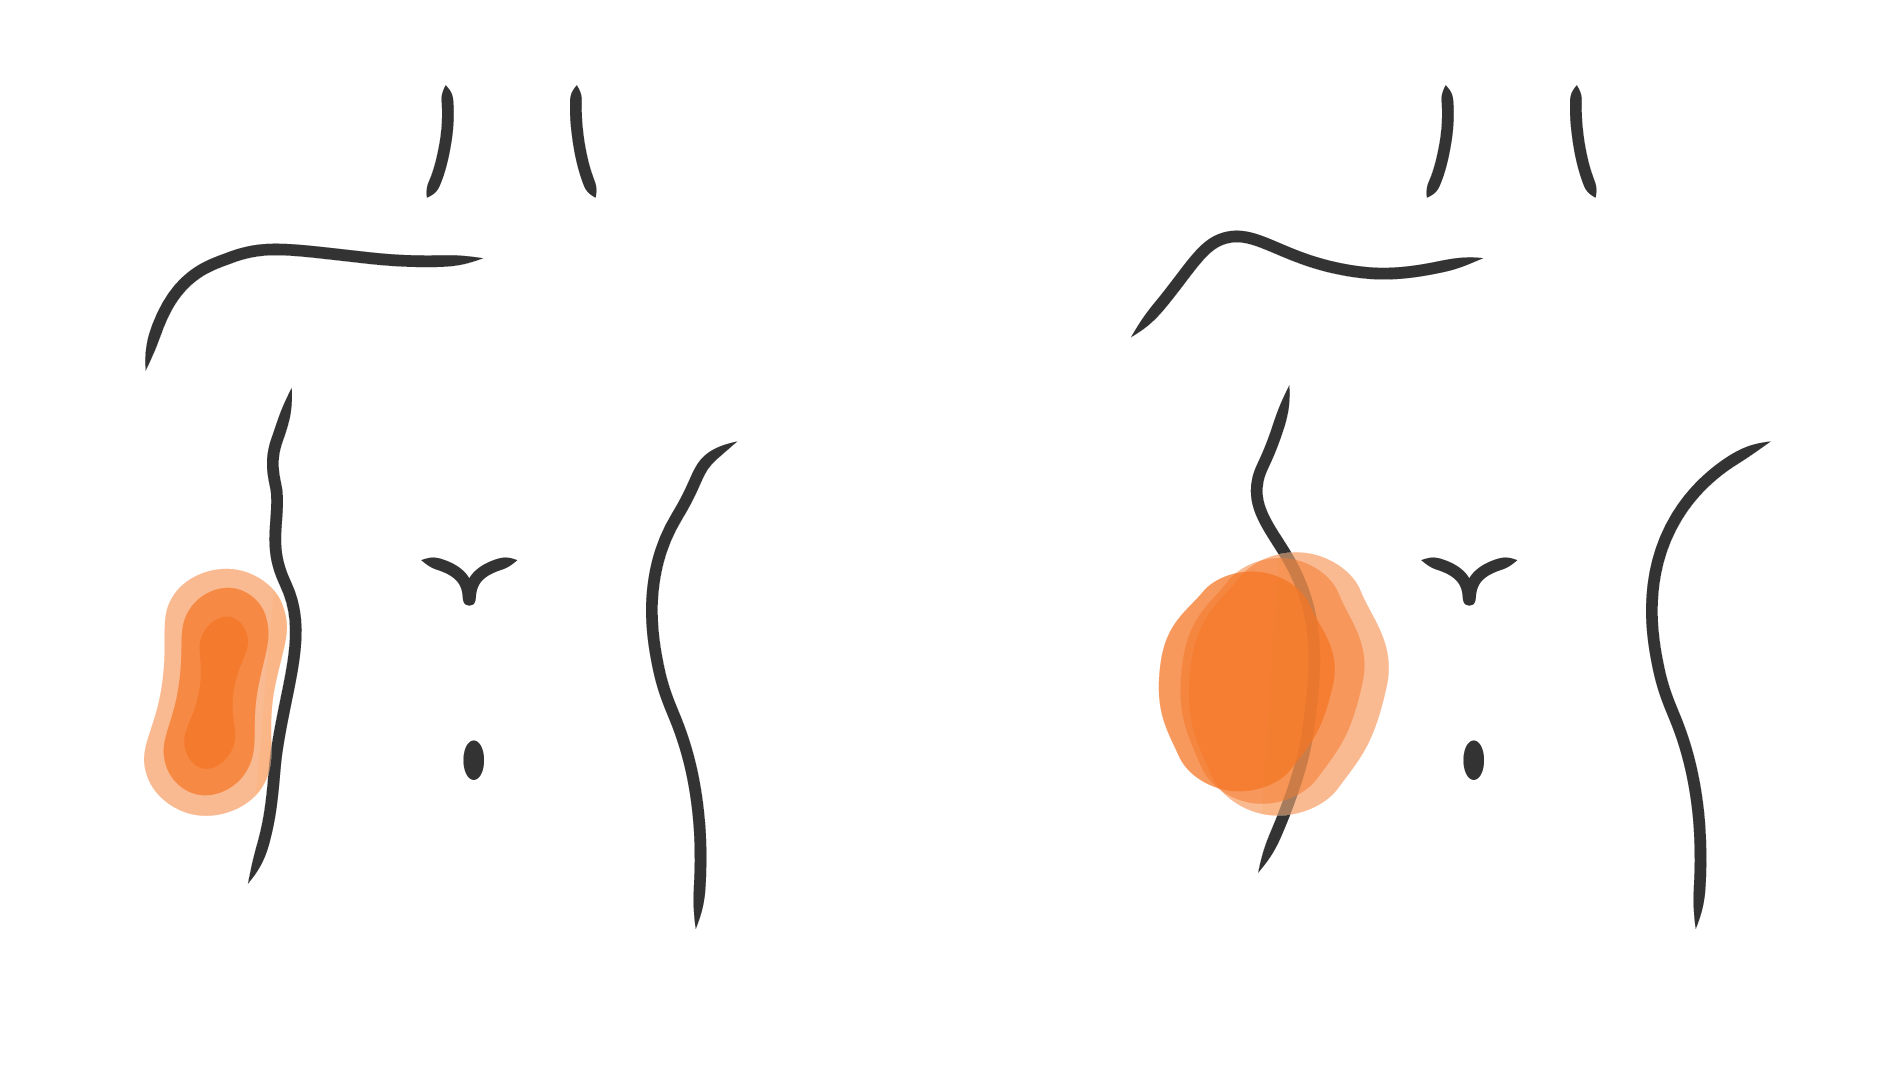
\includegraphics[width=0.9\textwidth]{Chapters/Figures/soma_chi/deep_pressure_graphic-01.png}
  \caption[Deep pressure, pressing onto the torso]{Deep pressure, pressing onto the torso, first using weak (left) and then strong pressure (right).}
  \label{fig:teaser}
%   \Description[Applying varying pressure on the right side of the abdomen]{Small orange shapes applying deep pressure to the right side of a person's abdomen, first using weak and then strong pressure}
\end{figure*}

The following sections will report on the outcomes contained in the publication that was delivered during the doctorate programme, including personal contributions as respective co-authors:

\printpublication{jung_exploring_2021}

We present the outcomes of a collaborative research effort between ourselves at PLUX Wireless Biosignals (M. Alfaras and W. Primett) and KTH Royal Institute of Technology (A. Jung, P. Karpashevich and K. Höök) merging resources from industry and academia representatives. The other authors will be mentioned by name to specify the responsibility of specific research actions, where appropriate.

This effort was observed over three guest research periods involving M. Alfaras, W. Primett, A. Jung each being hosted by the partnering institutions respectively for 1 to 2 months between. The hosting of A. Jung was partially interrupted in March 2020 due to the first COVID-19 pandemic. The resulting article encompasses a detailed view of the fabrication and technical composition of the actuation wearable produced. In the scope of this thesis, we will take this opportunity to highlight. the core insights taken from the user study, and use this to establish an aesthetic framework that holds relevance throughout the comprehensive research goals.

% \section{General Overview}
% \begin{center}
% \begin{tabular}{ p{13cm}}
% Deep Pressure Therapy relies on exerting \textit{firm touch} to help individuals with sensory sensitivity. We performed first-person explorations of deep pressure enabled by shape-changing actuation driven by breathing sensing. This revealed a novel design space with rich, evocative, aesthetically interesting interactions that can help increase breathing awareness and appreciation through: (1) applying symmetrical as well as asymmetrical pressure on the torso; (2) using pressure to direct attention to muscles or bone structure involved in different breathing patterns; (3) apply synchronous as well as asynchronous feedback following or opposing the user's breathing rhythm through applying rhythmic pressure. Taken together these explorations led us to design (4) \textit{breathing correspondence interactions} -- a balance point right between leading and following users' breathing patterns by first applying deep pressure -- almost to the point of being unpleasant -- and then releasing in rhythmic flow.
% \end{tabular}
% \end{center}

% \subsection{Introduction}
\section{Breathing Correspondence: Shape-changing Actuation for Breathing Awareness}

This study follows our explorations towards biofeedback systems for breathing and shape changing actuation that was initiated in the preliminary actions (Chapter \ref{cha:Preliminary_Actions_sens_act}) in addition to the work contained in the publications efforts that proceeded \cite{sanches_ambiguity_2019, alfaras_biodata_2020}. These modalities have been given attention by interaction design researchers, showcasing examples of breathing feedback as visual or aural representation, with other cases using haptic feedback with various tangible media, such as shape-changing materials \cite{prpa_inhaling_2020, miri_piv_2020}. We also note the technical progressions towards new shape-changing materials that have complimented this research \cite{coelho_shape-changing_2011}, however, there still remains a call for understanding their aesthetic potential of these systems from the perspective of the user \cite{rasmussen_shape-changing_2012,alexander_grand_2018}.

Deep Touch Pressure (DTP) is used in sensory integration therapy used for treating deficits in tactile stimuli \cite{bundy_sensory_2002}, making use of weighted garments and blankets, swaddling, or firm hugs to provide a firm pressure sensation to the body. Its calming effect seems to be due to stimulation of the parasympathetic nervous system, which plays a significant role in anxiety management \cite{hsin-yung_chen_physiological_2013}. In therapy practice, DTP has been applied to increase attention \cite{fertel-daly_effects_2001} and reduce anxiety symptoms \cite{krauss_effects_1987}, particularly for children and students with autism spectrum disorders (ASD) \cite{lang_sensory_2012,alfaras_espinas_making_2021}. So far, DTP is relatively unexplored in interaction design research (with some notable exceptions \cite{delazio_force_2018, duvall_dynamic_2019, foo_user_2019, foo_soft_2020}). We take deep touch pressure as a starting point for aesthetic qualities of coupling shape-changing pads with respiratory sensing, enabling the actuation materials to exert pressure on different locations on the torso of the breathing body.

% Our work builds on prior work combining biosensing and embodied exploration of actuation to focus on material properties \cite{sanches_ambiguity_2019, alfaras_biodata_2020} and display bodily reactions as they unfold in real time \cite{umair_towards_2019}.
The design process involved a series of collaborative design sessions engaging with couplings of breathing and pressure, construction of an experiential artefact \cite{sundstrom_experiential_2011} to explore the affordances of the socio-digital material, as well as long-term first-person explorations of the impact of shape-changing deep pressure feedback coupled with conscious breathing practices. This was done in different teams formed by the authors of the corresponding publication \cite{jung_exploring_2021}.
% The first author spent a total of 5 months systematically exploring placement and interactive behaviours with two other authors, while the two remaining authors explored a slightly different version of the deep pressure material on and off during a period of one year.

Through a process of material experimentation, we uncover potential for a number of novel interaction qualities that we will report on here: perceptual differences of applying deep pressure \textit{symmetrically and asymmetrically} on the torso and how these may help to increase breathing awareness; opportunities for \textit{directing attention} to different parts of the breathing apparatus, such as the bone structures or muscles involved, and thereby supporting learning a richer breathing repertory; the effects of providing feedback \textit{synchronously and asynchronously} in harmony with, contrary to, or even out of sync with the user's breathing rhythm leading to a deeper aesthetic appreciation of one's breathing; as well as exploring the balance point between letting the system subtly \textit{lead or influence} breathing patterns versus solely \textit{following} the rhythm of the user's breathing in the interactions -- an experience we will refer to as \textit{breathing correspondence}. These explorations contribute to opening up the design space around shape-changing interfaces by characterising potential experiential qualities and affordances based on felt bodily experiences of deep pressure for breathing awareness.

%%%%%%%%%%%%%%%%%%%%%%%%%%%%%%%%%%%%%%%%%%%%%%%%%%%%%%

\section{Background}

\subsection*{Breathing Awareness}

A growing body of research in HCI focuses on designing interactive systems to extend breathing awareness. Prpa and colleagues \cite{prpa_inhaling_2020} provide an overview of the underlying theoretical frameworks and design strategies used in breathing-based interactions. While some aim to trigger physiological responses related to alleviating stress and anxiety by slowing the breathing rate \cite{van_rooij_deep_2016, bumatay_investigating_2017, parnandi_chill-out_2014}, others utilise breathing patterns to promote mindfulness \cite{pisa_towards_2017, shamekhi_breathe_2018} or to support communication between people through synchronization of breathing \cite{desnoyers-stewart_jel_2019,kim_breathingframe_2015}. The somaesthetic design approach \cite{hook_designing_2018}, which informed our work, utilises breathing as gentle guidance to develop sustained attention towards bodily sensations and learn to appreciate all the nuances of the felt experience of breathing \cite{prpa_attending_2018, stahl_soma_2016}. By cultivating bodily and breathing awareness, users can come to better understand the connections between their physical and emotional experiences, thereby finding novel paths to regulate emotion and develop a higher sense of trust of their own body \cite{bornemann_differential_2015}.

Many of these systems capture breathing data and translate it into sensory stimuli to externalise breathing, making it visually or tangibly accessible to users, creating immersive virtual and physical environments for engaging with breathing practices from mindfulness, yoga, Feldenkrais \cite{moran_exopranayama_2016, patibanda_life_2017, vidyarthi_sonic_2012, stahl_soma_2016, shamekhi_breathe_2018} and other body practices. While most interactions address auditory or visual modalities, there have been a few tangible designs which mirror or guide users' breathing processes, such as fidget spinners with added visual feedback \cite{liang_biofidget_2018}, shape-changing airbags \cite{yu_breathe_2015} or stuffed animals \cite{aslan_hold_2016}. Other haptic systems mainly use vibration feedback \cite{dijk_breathe_2011,bumatay_investigating_2017, miri_piv_2020}, while other forms of immediate haptic feedback on the torso have so far rarely been explored with the exception of a recent study by Foo et al. \cite{foo_soft_2020}. They noted that rhythmic pulsing compression applied on the torso showed potential to improve focused attention on breathing and adopt a slow breathing rhythm, making it an interesting option for further exploration.

\subsection*{Shape-Changing Interfaces}

Shape changing interfaces constitute a novel interaction form as they enable interactive changes of the shape or texture of a material \cite{alexander_grand_2018}. The increasing maturity of these shape-changing materials and tangible technologies has led to increased attention in the HCI and interaction design field. Recently, we have seen several attempts to clarify what this design space offers when building applications. For instance, Coelho and Zigelbaum \cite{coelho_shape-changing_2011} try to characterise technological properties of shape-changing materials, while Rasmussen and colleagues \cite{rasmussen_shape-changing_2012} identified eight different types of shape changes of relevance to different functional and hedonic design purposes. Others present particular design exemplars, including mobile devices \cite{hemmert_shape-changing_2010, dimitriadis_evaluating_2014, gomes_morephone_2013}, interactive tabletops \cite{follmer_inform_2013, taher_exploring_2015}, furniture \cite{gronvall_causing_2014}, toys \cite{katsumoto_ninja_2013}, and interactive architecture \cite{oosterhuis_interactions_2008}. A few shape-changing design exemplars have addressed breathing, such as a stuffed animal breathing in synchrony with its user \cite{aslan_hold_2016}, a photo frame  reflecting a partner's breathing \cite{kim_breathingframe_2015}, or morphing physical environments for engaging with one's own breathing \cite{sjoman_breathing_2018, schnadelbach_exobuilding_2012}. These systems mainly emphasise the visual aspect of shape-changing interaction \cite{kim_breathingframe_2015, sjoman_breathing_2018, schnadelbach_exobuilding_2012, moran_exopranayama_2016}, and only in a few cases are they used to produce tactile feedback \cite{yu_breathe_2015} or engaging with users' movements \cite{tomimatsu_breathing_2016}.

In comparison to the technical development, the aesthetic user experience of interacting with shape-changing materials as well as their affordances have not received as much attention \cite{rasmussen_shape-changing_2012, alexander_grand_2018}. Rasmussen and colleagues \cite{rasmussen_shape-changing_2012} devised two types of expressive parameters to characterise how movements of shape-changing interfaces are perceived by users. These include adjectives like smooth or angry as well as associations, such as a phone expressing sadness through a human-like sobbing pose. Due to their dynamic characteristics, users and designers often use metaphors to describe shape-changing behaviours, associating them with certain personality traits, animals or ascribing them other life-like qualities \cite{rasmussen_sketching_2016, kwak_design_2014}.

\subsection*{Deep Touch Pressure}

Deep touch pressure (DTP) is a method used in sensory integration therapy, aimed at treating sensory processing difficulties related to, amongst others, anxiety disorders, in particular anxiety experienced by those on the autism spectrum \cite{hsin-yung_chen_physiological_2013, grandin_calming_1992, krauss_effects_1987}. The therapy involves using tools such as weighted garments and blankets to provide a comforting pressure sensation. Its calming effect can be attributed to increased activity of the parasympathetic nervous system, which plays a significant role in anxiety management \cite{hsin-yung_chen_physiological_2013}. In therapy practice, DTP has been applied to increase the ability to focus \cite{fertel-daly_effects_2001}, reduce disruptive behaviour \cite{quigley_effects_2011} and reduce anxiety symptoms \cite{grandin_calming_1992} in patients with bipolar disorder, developmental disorders and those on the autism spectrum.

In HCI, different types of compression garments have been developed to provide DTP. Vaucelle et al. \cite{vaucelle_design_2009} designed a pressure vest containing pneumatic chambers. A more elaborate project is the Force Jacket \cite{delazio_force_2018}, an upper body garment that uses pneumatically-actuated airbags to create sensations of directly applied force and high frequency vibrations. Such vests are the most common form of designs for deep touch pressure and make up the majority of commercially available DTP products, such as the Tjacket \cite{ltd_tjacket_2020} or the Squease vest \cite{ltd_squease_2014}; both are inflated using external pumps. Such vests have also been used to simulate hugs in long-distance interactions between parents and children \cite{teh_huggy_2009}.

% An alternative type of pressure garment uses shape memory alloys which contract when heated, exerting pressure on the wearer’s body \cite{duvall_dynamic_2019}. Foo et al. \cite{foo_user_2019} evaluated the user experience of compression garments based on shape memory alloys. They found that while individual preferences regarding different temporal patterns of pressure varied, it was overall experienced as more comfortable on the torso than on the shoulders or arms. Users reacted more sensitively towards pressure on the upper back than on the lower back, and felt that lower back compression supported their posture. The compression garments created a calming and warm effect, making participants feel secure and comforted.

% The work we present here takes off from these earlier explorations, deepening prior work through exploring the aesthetic potential of deep pressure interactive shape-changing materials applied on and around the torso.


%%%%%%%%%%%%%%%%%%%%%%%%%%%%%%%%%%%%%%%%%%%%%%%%%%%%%%
%% DESIGN PROCESS
\section{Design Process}
\label{subsec:chi_soma_design_process}

% \begin{table*}
% \caption{Researchers' demographics (as of January 2021).}
% \begin{tabular}{ l| c c p{0.4\linewidth} }
% \textbf{Name} & \textbf{Gender} & \textbf{Age} & \textbf{Design and research background} \\ \midrule
% Annkatrin & Female & 23 & M.Sc. in human-computer interaction and design, 8 months experience with soma design \\
% Miquel & Male & 31 & Graduate student in computer science, 1 year experience with soma design \\
% Pavel & Male & 32 & Graduate student in interaction design, 3.5 years experience with soma design \\
% William & Male & 24 & Graduate student in sound-movement interaction, 2 years experience with somatic practices \\
% Kristina & Female & 56 & Professor in interaction design and expert in soma design\\
% \end{tabular}
% \label{table:demographics}
% \end{table*}

Our design work started with a general interest in deep touch pressure, but when extrapolating from this concept we came to explore a range of interactions between physical pressure and breathing. Our explorations were done from an embodied, first-person perspective \cite{hook_embracing_2018}, putting the researchers themselves, their movements and subjective experiences at the centre of the design process.
% All five authors participated in this design process at different stages, in different constellations and with different variations of  technological setups. Their demographic information is summarised in Table \ref{table:demographics}.

The process was initiated by the author Annkatrin \cite{jung_exploring_2021} via initial exploration of the breathing sensor, shape-changing actuators and fabrics for creating restriction and shape-change. This initial phase lasted for 1.5 months and allowed for discovering the affordances and experiential qualities of the available technology and materials, as well as experimenting with different shapes and sizes of the inflatable elements. Her first insights from this process informed possible interactions with different actuator sequences, which were further explored in a series of collaborative soma design workshops \cite{hook_designing_2018} performed by researchers Annkatrin, Miquel and William (thesis first author).
% These workshops are detailed in section \ref{sec:soma_workshops}.
In total, four sessions took place over three weeks, iteratively exploring opportunities for connecting different actuation sequences and breathing techniques in relation to different areas of the body. The soma design workshops were followed by a continued systematic exploration of the deep pressure coupled with specific breathing techniques done by Annkatrin over a period of two months. This led to the construction of a wearable garment which places the shape-changing actuators on the upper and lower back to guide different ways of breathing, as shown in Figure \ref{fig:garment}.

% Annkatrin engaged with the garment daily over a period of three weeks (detailed in section \ref{sec:first_person_engagement}). In parallel, two other authors (Pavel and Kristina) explored a similar setup with identical shape-changing actuation and inflatable pillows encapsulated in the restrictive torso garment, but focused primarily on actuation. This design work took place over a one-year period and involved two somatic connoisseurs - a Feldenkrais expert and a professional singer - who helped to devise breathing techniques for the device and facilitated a richer understanding of the perceived bodily sensations of the interactions.

The results discussed in this study are primarily based on the series of soma design workshops performed by the authors of the corresponding publication, Annkatrin, William and Miquel, as well as the further investigation of specific breathing techniques done by Annkatrin afterwards. This was also complimented with additional insights from the design work done by Pavel and Kristina.

\subsection*{Soma Design Sessions}
\label{sec:soma_workshops}

Over the course of four weeks, Annkatrin, William and Miquel performed a series of four collaborative soma design workshops exploring breathing-based interactions with shape-changing pressure feedback. The three authors are actively engaged in the field of embodied interaction with biofeedback systems, carrying modest experience with bodily practices such as yoga and Feldenkrais through regular practice both in and out of the lab. An additional participant, a graduate student from a product design background who is not among the authors of this paper, joined in the third session.

The workshop structure was grounded in soma design theory which places sensory experiences and appreciation at the centre of the design process to incorporate the soma, the integrated whole of body and mind, in a holistic manner and build a subjective understanding of one’s somatic experiences \cite{hook_designing_2018}.
% Soma design methods focus on gaining awareness of physical experiences, exploring materials through embodied interaction, and testing out possible sensations first-hand, emphasising a first-person, autobiographical perspective \cite{hook_embracing_2018, neustaedter_autobiographical_2012}.

%  \begin{figure}[b]
%   \centering
%   \includegraphics[width=0.62\linewidth]{Chapters/Figures/soma_chi/actuators.png}
%   \includegraphics[width=0.28\linewidth]{Chapters/Figures/soma_chi/torsosides.png}
%   \caption{Researchers' demographics (as of January 2021).}
%   \label{fig:inflatables}
%   \Description[Shape-changing actuators in different sizes, strapped to the sides of the torso]{One actuator device with several pillows in different shapes and sizes. Two equal-sized pillows were strapped to either side of the torso during a soma design workshop.}
% \end{figure}

Each of the four sessions lasted about three hours including the setup and incorporated shape-changing actuators in various shapes and sizes, as well as additional fabrics to attach them to different parts of the body and create restriction. The actuators are part of the Soma Bits toolkit \cite{windlin_soma_2019}, a collection of shapes and actuators designed to facilitate soma design workshops, and consist of Thermoplastic Polyurethane (TPU)-coated nylon shapes which can be inflated or deflated at different speeds or stay at a constant level of inflation. Further in the text, we will be using ``pillows'', ``inflatables'', ``pneumatic pads'' interchangeably to describe these shapes. The actuation was controlled wirelessly with an Arduino-based device, capable of inflating and deflating the pneumatic pads at variable pump speed (max 3L/min) within the pressure range of 450 - 1950 hPa, as well as providing real-time pressure sensor readings.

The framework used for sensing and actuation control is illustrated in Figure \ref{fig:workflow}.
To capture breathing, we used an inductive respiration (respiratory inductance plethysmography, described in Section \ref{sec:sensing}) sensor\footnote{\url{https://biosignalsplux.com/products/sensors/respiration-inductive.html}} (1) which measures the relative displacement of the chest or stomach, depending on its placement. The sensor data is continuously acquired to compute the subject's breathing rate, which in turn influences the time dynamics of the shape-changing feedback. This data exchange is handled by (4) a Processing server, directing control messages between the browser-based Node-RED GUI (2) and the actuation hardware (5 \& 6) via Open Sound Control (OSC). The visual interface allows for the different actuation sequences to be executed with adjustable parameters, while a separate Python script runs in the background for signal processing and feature extraction (3).

\begin{figure*}[t]
    \centering
    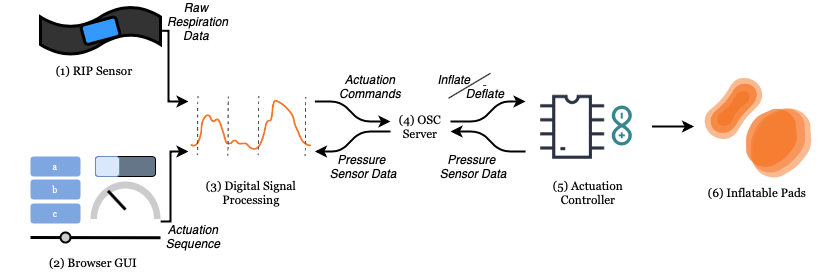
\includegraphics[width=1.0\linewidth]{Chapters/Figures/soma_chi/fig_2_framework.png}
    \caption{Modular framework for sensing and actuation control.}
    \label{fig:workflow}
    % \Description[Components of the framework for sensing and actuation control]{All components of the framework for sensing and actuation control are shown in a flow chart.}
\end{figure*}

% As soma design work incorporates bodily practices such as Feldenkrais and body scans to improve designers’ somaesthetic awareness, e

Each workshop began with a somatic practice to cultivate a sensitivity towards the bodily sensations, placing the aesthetic experiences in the foreground of the embodied interaction. This was specifically structured as a Feldenkries routine, focused on breathing and micro-movements. Afterwards, the participants took turns in placing the pads on different parts of their bodies to investigate how different placements, actuation sequences and body positions influence the experience. The explorations followed the soma design method of making strange \cite{loke_moving_2013}, deconstructing habitual movements to draw attention towards subtle sensations and create a richer understanding of the experience.

In addition to taking notes, pictures and videos during the workshop, the participants used soma body sheets to document and visualise their subjective bodily experiences \cite{candy_intimate_2014}, the drawings were used to aid discussion into the felt bodily sensations that occurred throughout the session. These sheets depict an empty outline of a human body onto which one can draw and write how they are experiencing different parts of their body, as shown in Figure \ref{fig:bodysheets}. These sessions enabled the authors to narrow down the physical schematics that would facilitate meaningful interactions. They included a set of suitable pad shapes/sizes and bodily placements that could be embedded into a wearable interactive system.

% A reflection period amongst the participants concluded each session.

\begin{figure}[b]
  \centering
  \includegraphics[width=0.80\linewidth]{Chapters/Figures/soma_chi/Bodysheet_highres.png}
  \caption[Example of a body sheet]{Example of a body sheet used to document the somatic experience during the design process.}
  \label{fig:bodysheets}
%   \Description[From feeling shaky and stiff before the exploration to building an asymmetric awareness of the body]{A body sheet showing the changes of the somatic experience before and after a soma design workshop. Before, the participant felt shaky and stiff, aware of a heavy feeling in the arms and a single-point contact of the feet. Afterwards, the participant experienced an asymmetric awareness of the body: The left side felt caged, while the right side was more connected, flexible but tough, and with a stronger flow of energy. The feeling in the feet was forgotten after the workshop.}
\end{figure}

\subsection*{Autobiographical Design: First-Person Engagement with Shape-Changing Materials and Breathing}
\label{sec:first_person_engagement}

Based on the insights obtained during the soma design workshops, Annkatrin created a restrictive garment which contains the shape-changing pads, pressing against both the upper and lower back. It was inspired by the design of similar compression garments \cite{vaucelle_design_2009, foo_user_2019}, but not intended to represent a final design outcome nor a prototype for deep touch pressure therapy. Instead, the garment acted as an experiential artifact \cite{sundstrom_experiential_2011}, an intermediate tool in the design process to present new and interesting experiences and discover their affordances through embodied interaction with breathing-based deep pressure.

 \begin{figure*}[t]
  \centering
    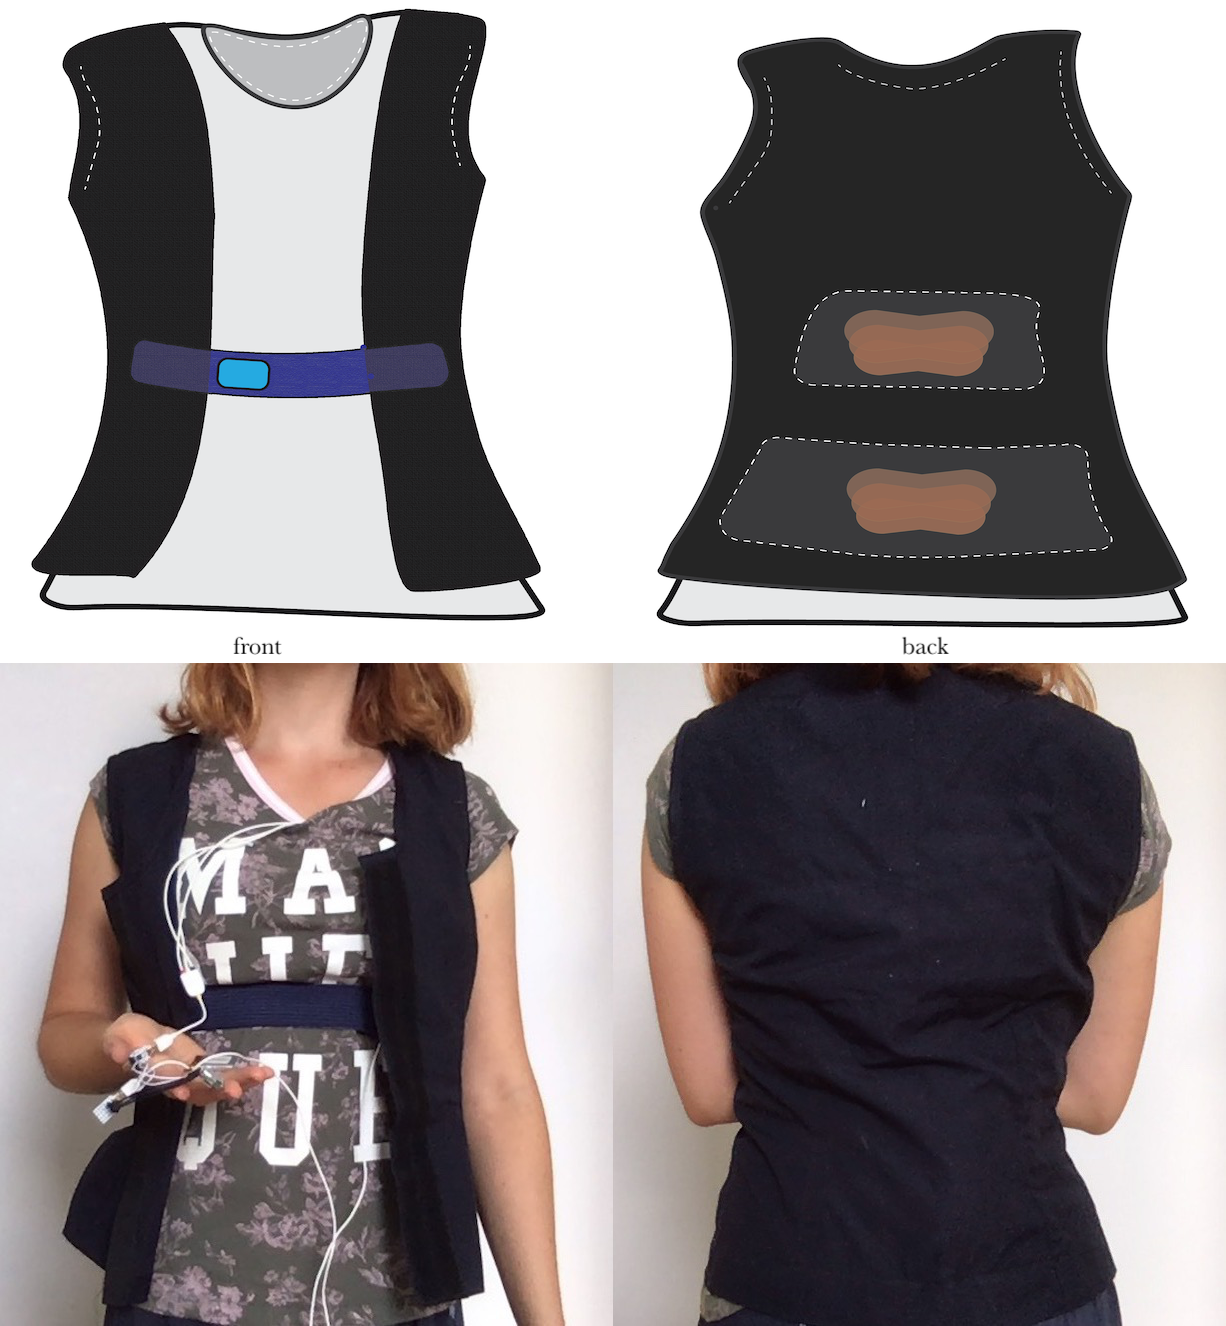
\includegraphics[width=0.8\linewidth]{Chapters/Figures/soma_chi/fig_5_all_grid.png}
  \caption{The garment, worn with a breathing sensor and one pad in each inner pocket.}
  \label{fig:garment}
\end{figure*}

Figure \ref{fig:garment} shows the breathing garment being worn. A respiration sensor is strapped around the torso underneath the garment. On the inside, two pockets are attached on the upper and lower back. Each pocket holds one inflatable pillow to apply deep pressure on different areas of the back. When closed, the garment fits tightly and can transfer the deep pressure applied by the pads. The outer material can be closed in the front with a loop-and-hook fastener which allows for a tight fit in the torso area, making the actuation clearly noticeable. The pads can be placed in two pockets on the inside of the garment, one on the lower and one on the upper back. We would like to note that the garment needs to be closed to apply deep pressure and is left open in Figure \ref{fig:garment} to show the placement of the respiration sensor.

% During the exploration, the actuator devices were placed externally and connected to the pads in the garment via two elastic air hoses that are laced through a small hole at the bottom of the lower pocket. Although this constrained Annkatrin's movements within a small area around the actuators and required her to be careful when changing position, it did not detract from the interaction with the garment. The sound of the air pumps was dampened using noise-cancelling headphones playing white noise.

% The garment was used along with an inductive respiration sensor to explore deep pressure feedback combined with different breathing techniques. The sensor was worn around the chest or stomach underneath the garment. Over the span of three weeks, Annkatrin conducted one to two sessions daily with a duration of 30-60 minutes each. These sessions were focused on exploring the potential impact of shape-changing deep pressure feedback coupled with a regular conscious breathing practice over a longer period of time on the subjective bodily experience and breathing awareness.

The sessions incorporated different breathing techniques as well as different contexts and positions, including lying on the back, sitting on a chair or doing other tasks such as reading or writing while wearing the garment. These positions and breathing patterns were informed by a two-months systematic exploration of deep pressure guiding different kinds of breath regulation, such as controlling the duration of inhalations and exhalations or alternating between diaphragmatic and thoracic breathing, done by Annkatrin in between the soma design workshops and the construction of the garment.

In total, four different breathing techniques were used:
\begin{enumerate}
    \item 5.5 pattern: Providing a constant rate of 5.5 inflate-deflate cycles, i.e. breaths, per minute, which has been associated with increased heart rate variability and relaxation \cite{lin_breathing_2014}.
    \item Three-part breath pattern: This was inspired by the three-part breathing technique from yoga \cite{sengupta_health_2012} which combines diaphragmatic and thoracic breathing. One pad is placed on the lower and one on the upper back. The one on the lower back is inflated first followed by the one on the upper back, guiding the user to first fill the stomach with air and then let it expand into the rib cage and chest. Then, the pad on the upper back is deflated again followed by the one on the lower back, guiding the user to release the breath first from the chest and then the stomach. Each inflation and deflation interval has a duration of 2 seconds, with a 1 second pause in between breaths.
    \item Standardised feedback based on breathing sensor data with a 2 second pause in between breaths: It mirrors the user’s breathing intervals, multiplied by 1.7 to gradually increase the duration of one breath without making the difference between two successive intervals too large.
    \item Adaptive feedback with an actuation change triggered by rapid breathing: At baseline, the inflation speed is set to 50\% of the maximum, which makes the pads less noticeable. If the calculated inhale or exhale duration is shorter than 2 seconds, the inflation speed is increased to 100\% until the breath becomes longer again.
\end{enumerate}

At the beginning of each session, Annkatrin conducted a short body scan to take note of her present bodily sensations and breathing. Then, Annkatrin explored each combination of actuation pattern and position or context for at least 20 minutes before moving on to the next to experience more long-term effects of each condition. A single session was focused on a maximum of two different actuation patterns or two different body positions.

The exploration was documented in the form of an online diary as an intermediate step in the process of articulating the experiences. Initial impressions of the effects of the breathing exercises and the pressure feedback on the breathing and bodily experience as well as notable changes in the inductive respiration sensor data were noted down quickly and informally. As it was often difficult to articulate the primarily bodily explorations while still immersed in the process, it was necessary to take a short break afterwards before reflecting more deeply on the experiences based on the initial notes.

%%%%%%%%%%%%%%%%%%%%%%%%%%%%%%%%%%%%%%%%%%%%%%%%%%%%%%
%% EXPERIENTIAL AESTHETIC QUALITIES

\section{Experiential Aesthetic Qualities}
\label{sec:aesthetic_qualities}

In the following, we present the four experiential aesthetic qualities that grew out of our design explorations. Such qualities bring out the aesthetic potential of interactions and how they are experienced in use \cite{lowgren_toward_2009}, serving as an abstraction tool to articulate the insights which emerged over a series of explorations \cite{stahl_evocative_2014}. These qualities coincide with general aesthetic criteria that has been established in Section \ref{cha:aestheitic_parameters}, characterised as spatial or temporal sensations that can be applied universally across all sorts of mediums.

Each quality is introduced with a body of examples that highlight how the quality manifested in different first-person interactions. In reflection of these accounts and the data collected in the design explorations, we then outline the aesthetic potential of shape-changing deep pressure feedback and the overall influence this had on different breathing techniques. We discuss how pressure-based feedback can be used to cultivate breathing awareness, appreciation, controllability and deconstruction. The different experimental configurations allowed us to document a range of experiences relating to our breathing patterns, some yielding a greater awareness by reinforcing our habitual behaviour, and others disrupting the familiar movements.
%

\subsection*{Placements on the Torso -- Symmetric versus Asymmetric}

Insights of the importance of symmetrical as well as asymmetrical feedback arose from how the inflatable pads could be moved around to different locations on the torso. This made it possible to put deep pressure on, for example, the back right shoulder at the same time as another inflatable put pressure on the lower left-side of the belly. By symmetrical feedback, we are referring to pressure applied equally on the left and right sides of the torso, i.e. symmetrical on the lateral plane with the same actuation pattern. Asymmetrical feedback refers to one-sided pressure or pressure on both sides of the body, but a) on different body parts or b) with different actuation patterns.


\subsubsection*{Experiencing symmetric and asymmetric feedback}

The team's explorations naturally began with symmetrical placements, leading to a whole range of interesting experiences. For example, when Annkatrin was experimenting with placing the inflatable pillows symmetrically on both shoulders, as shown in Figure \ref{fig:neck}, position (1), she experienced massage-like qualities or \textit{``someone putting a comforting hand on your shoulder''}. When placing the pads near the lower back or waist area when sitting or lying down, the pressure created a sense of support and stability. This was especially pronounced when placing the pads on either side of the lower back in a lying position, forming \textit{``a small indent in the floor to enclose my body, causing a comfortable and safe feeling''}. Annkatrin reported feeling unsteady and in lack of 'support' when the pillows were taken out or deflated, as if she would \textit{``roll to the left or right side at any moment''}. The symmetrical placement of the pads under the body was often helping Annkatrin to \textit{``feel more connected to the floor, more grounded in my body and my environment''}. Generally, interactions with symmetrical placements and patterns invoked calm and relaxed feelings: \textit{``I was left feeling much more in touch with my body, more calm and centred in myself. I felt loose, relaxed and a bit sleepy, similar to how I feel after a yoga practice or a good workout''}.

Inspired by Feldenkrais exercises, Annkatrin, William and Miquel went on to experiment with asymmetrical actuation during the design workshops. Many Feldenkrais lessons aim to deconstruct the habitual coordination of movements. It is done in order to draw attention to their finer details or offer novel ways in which movement can be created, ultimately leading to alternative habitual movement patterns. Based on those Feldenkrais lessons, Annkatrin, William and Miquel tried to re-create a similar feeling of imbalance or deconstruction by placing the pillows on only one side of the body or putting two pillows simultaneously on different body parts. This created two different effects: while applying the actuation to two different body parts made it \textit{``hard for us to decide where to direct our attention which created an ill-fitting, incongruous experience''}, concentrating on only one side of the body \textit{``allowed us to become more aware of how we experienced that specific body part''}.

Later, Annkatrin continued to experiment with asymmetric actuation using two pads with conflicting or complementing rhythmic patterns at the same time. As opposed to random or conflicting feedback, we define \textit{complementing asymmetric feedback} as requiring a regularity of sorts: the actuation intervals of one pad can be a multiple of the second pad, or one pad inflates while the other deflates. A \textit{conflicting pattern}, on the other hand, has incoherent phases, switching from inflation to deflation at different times. These explorations revealed that \textit{``the placement of the pads had to be matched carefully to the actuation''} to avoid interfering with each other or with the user's breathing. In particular, conflicting asymmetric actuation was perceived as distracting and uncomfortable, not leading to any deeper engagements. For example, placing the inflatables on the back of the thighs or using two very distinct actuation sequences \textit{``failed to evoke any strong effect''}. In some cases such placements could even lead to strong negative experiences, preventing learning. Placing the pads asymmetrically close to the neck, as shown in Figure \ref{fig:neck}, position (2), made Annkatrin feel \textit{``like I was not able to breathe properly''}, evoking associations with \textit{``having a snake wrapped around my throat''}. On the other hand, when the position and patterns were complementing -- for example, when Annkatrin tried putting two pillows with one inflating twice as fast as the other on the lower back (Figure \ref{fig:neck}, position (3)) -- they \textit{``created a very unusual twisting sensation in the torso''}. This in turn lead to insights on how locally applied effects can spread across the entire body, and helped Annkatrin to experience how different parts of the body are connected into a whole.

 \begin{figure}[t]
  \centering
  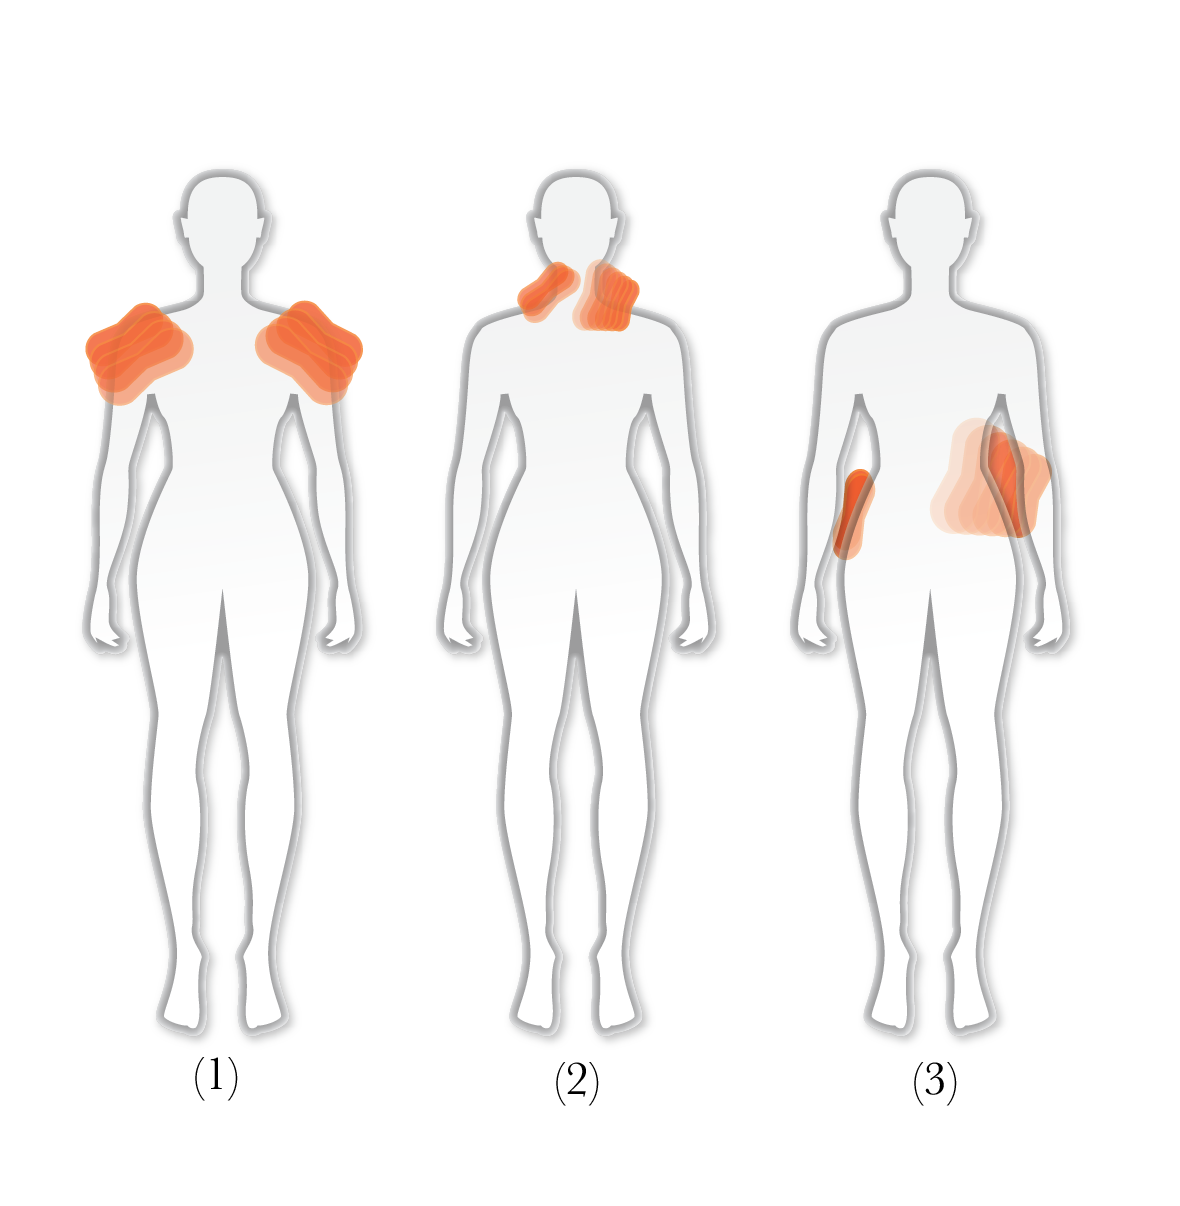
\includegraphics[width=0.65\linewidth]{Chapters/Figures/soma_chi/fig6_positions_numbers.png}
  \caption[Applying symmetric and asymmetric deep pressure]{Applying symmetric and asymmetric deep pressure to the shoulders (1), neck (2) and lower back (3).}
    \label{fig:neck}
    % \Description[Applying symmetric and asymmetric deep pressure to the shoulders, neck and lower back]{Applying symmetric deep pressure to the shoulders, as well as asymmetric deep pressure to the neck and lower back. In the latter case, pressure is applied more strongly to the right side of the body.}
\end{figure}

\subsubsection*{Reflecting on symmetric and asymmetric feedback}

Symmetry is represented in many different forms in the HCI projects focused on breathing. In  projects with visual feedback, symmetry has been expressed as: visualization of two living lungs \cite{abushakra_augmenting_2014}; symmetrical  geometrical figures \cite{van_rooij_deep_2016, prpa_hacking_2016} or living virtual structures \cite{patibanda_life_2017} located in the centre of the screen or virtual environment; or as abstract symmetrical visualizations taking the whole computer screen \cite{moraveji_breathtray_2012}.
% One can see symmetry expressed as varying light intensity in the Philips LivingColor pair of lights \cite{dijk_breathe_2011}.
In the projects using vibration as output medium, symmetry is found in the relative position of the vibrating artefacts on the body, such as: centre of the belly \cite{bumatay_investigating_2017}; centre of the upper chest \cite{frey_breeze_2018}; or in the blanket that has the same vibro-tactile sensation on both sides of the body \cite{dijk_breathe_2011}. In projects using shape-changing actuation as a medium to display breathing, symmetry is found in: the equable expansion and contraction of a living wall \cite{sjoman_breathing_2018}; in dynamic building structures \cite{moran_exopranayama_2016, schnadelbach_exobuilding_2012}, as well as in the whole shape of a particular probe \cite{aslan_hold_2016, kim_breathingframe_2015}; or sometimes experienced by the whole body symmetrically \cite{sun_breath_2017}.

 \textit{Asymmetry} as a design quality of breathing feedback has not been explored as much. There have only been a few asymmetrical representations, such as a visualization of tides in the virtual garden \cite{roo_inner_2017}, and a few examples of providing direct feedback onto only one side of the body, such as the guiding shape-changing pillow under the right palm of the hand in the works by Yu and colleagues \cite{yu_breathe_2015}.

The focus on symmetrical representations in design work may be rooted in the notion that symmetry is commonly associated with perceived beauty and satisfying aesthetic experience \cite{nadal_study_2020, mcmanus_symmetry_2005}. Well-balanced presentations of equal proportions are more compatible with classical mathematical structures, and the link between symmetry and beauty even has explicit associations with our biological presence \cite{cardenas_symmetrical_2006}. However, absolute symmetry is not something we normally experience in the natural world, and leaves insufficient space for unpredictability and thereby discovery \cite{mcmanus_symmetry_2005}. We also note that the idea that symmetry is aesthetically pleasing is more prevalent in western culture \cite{nadal_study_2020, zeki_clive_2013}.

While we might perceive a human body as symmetrical when we compare our left half to our right half, it is obviously not. All the projects mentioned above in some way or other represent the lungs as a system with the perfect bilateral system. However, in a healthy individual, the left lung is slightly smaller than the right one to make some space for the heart -- as the heart is slightly shifted to the left. Our limbs are also asymmetric, often making one side of our body the more dominant one. Some of us are writing with our right hands, some with the left, and even ambidextrous people find it hard to use both hands for every habitual task. Our limbs are not perfectly equal -- there is often a limb length discrepancy. We are asymmetrical by nature and through training and everyday habituation, we might become even more asymmetrical in ways that harm us.

What then is the aesthetic potential of addressing these asymmetries in design? While symmetry and symmetrical feedback is a well-explored and articulated quality and approach, proven to be beneficial for creating feedback that is easy to grasp and follow, asymmetry has not been explored as much. What we found is also how asymmetrical feedback can be quite unpleasant and distracting. But when designed carefully, it can be very informative for the design process -- as well as to users aiming to increase their breathing awareness. What is sometimes needed is a journey from asymmetry to putting those asymmetrical experiences back into a symmetric whole, as is often done in Feldenkrais pracitce \cite{worth_symmetry_2015}. This is achieved by directing attention to just one side of the body, one lung, particular limb or other body part. For example, we might want to address the diagonal connection from the left lung into moving the hip on the right side, and then the connection from right lung to left hip movements, but then we need to put both together in order to explore and feel how all these parts are interconnected. If we leave the user with only one half of this experience, for example the connection from left lung to right hip, they might leave the exercise with a feeling of being lopsided.

% Merged above
% Asymmetry as a quality is widely used in Feldenkrais practice for disrupting the processes of the familiar \cite{worth_symmetry_2015}. In Feldenkrais lessons it is achieved by directing attention to just one side of the body, one lung, particular limb or other body part. This allows us to break the circle of habitual experience and reconstruct them bit by bit, slowly and attentively into something new -- evocative and unusual.

\subsection*{Guiding Different Kinds of Breathing}

There are many possible breathing patterns promoted by different physical disciplines and body practices. Some are specifically targeted at focusing the mind and increase bodily awareness \cite{kupershmidt_definition_2019, burke_role_2008}. To further explore the different muscles and bone structures involved in breathing, we decided to more deliberately impose deep pressure on different locations of the breathing apparatus in a manner that mirrors and encourages these different breathing patterns.

\subsubsection*{Experiencing breathing in different body parts}
Applying deep pressure to different locations on the body not only made it possible to explore symmetric vs asymmetric feedback, but also to feel the breathing in different body parts. The actuation was adapted to the user's breathing by inflating the pillows during inhalation and deflating the pillows during exhalation, including a slight delay as the user’s breathing intervals are computed from sensor data. This interaction is from here on referred to as \textit{following} the user's breathing.

The explorations started with taking conscious breaths through the chest while placing the inflatable pillows on and under different body parts which revealed their potential to physically move the body in certain directions. This led to a range of interesting experiences that were not necessarily related to breathing, such as placing them under the feet to cause a movement which Annkatrin related to \textit{``walking on the spot''}.

However, Annkatrin experienced breathing-based actuation mirroring her breathing on the lower body as \textit{``uncomfortable and unnatural since I could not relate those body parts to my breathing''}, which made her feel \textit{``weird, like it's not supposed to be there''}. Instead, the pressure was more readily associated with breathing when it was applied close to the breathing apparatus, i.e. on the torso or upper body. Annkatrin associated forward and upward movements of the torso with an inhalation, \textit{``the pads seemed to push me to inhale''}, while moving backwards and pressing down on the torso were perceived as an exhalation. Placing the pads underneath each armpit \textit{``pushed my arms away from the body''}, creating a feeling of the chest expanding during an inhalation. In this way, the pressure was able to support certain ways of breathing by reinforcing the respective movements. Annkatrin found that when the pads were placed under the lower back, the pressure \textit{``encouraged me to breathe more with my stomach''}, while placing the pads on the upper back \textit{``made me breathe more with my chest''}. Guided by the pressure, Annkatrin was able to learn how to engage different muscles when inhaling and thus practice diaphragmatic or thoracic breathing.

To investigate these different breathing patterns further, Annkatrin, as well as Pavel and Kristina in their explorations, created an actuation pattern based on the three-part breath, a technique from yoga practice which combines diaphragmatic and thoracic breathing in each inhalation and exhalation. Since this exercise requires a certain amount of awareness and control over which muscles are engaged when breathing, Annkatrin had to \textit{``focus a little more to direct my breath from my stomach to my chest and back''}. With one pad placed on the upper and another on the lower back however, she reported being able to follow the guidance of the deep pressure \textit{``without having to think about how I was supposed to breathe''}.

Over time, the exercises created a lasting effect which carried over into Annkatrin's everyday life: \textit{``I could feel the muscles in my torso more distinctively when walking around. I was experiencing my breathing more intensely throughout the day, leading me to take deeper breaths than before and use my stomach and chest more deliberately and distinctly while breathing''}. This suggests that by applying deep pressure on certain body parts, the pads may help improve someone's control of their breathing over time, stimulating engagement with certain muscles to assist different ways of breathing with regular practice. While three-part breathing is just one possible option, a plethora of techniques exist, such as letting the rib cage expand towards the arms, chest, back or shoulders when inhaling. Each of these directions engages different muscles around the rib cage, that, when trained, can open up a rich repertory of breathing techniques.
%

\subsubsection*{Reflecting on different kinds of breathing}

While many different muscles and bone structures are involved in breathing and enable distinct breathing patterns, breathing-based designs have mainly focused on reducing users' breathing rate \cite{prpa_inhaling_2020}. Whilst some of these studies account for lung capacity (e.g \cite{abushakra_augmenting_2014}), attention towards individual breathing muscles is normally ignored, neglecting the opportunity to practice alternative breathing patterns using these muscles.

Only a few breathing-based designs employ different types of breathing, for example encouraging deep diaphragmatic/abdominal breathing to alleviate stress \cite{prpa_hacking_2016} and anxiety conditions \cite{van_rooij_deep_2016}. Others measure breathing on different body parts \cite{prpa_attending_2018}, taking into account diaphragm expansion \cite{desnoyers-stewart_jel_2019} as well as the rising and falling extent of the abdomen \cite{schnadelbach_exobuilding_2012}.

Outside of HCI, a handful of studies validate the use of additional sensor placements in order to differentiate between thoracic and abdominal breathing, such as the work by Hamnvik and colleagues on Yolo4Apne \cite{hamnvik_yolo4apnea_2020} which uses two inductive respiration sensors and \cite{ejupi_detection_2018} that uses three resistive stretch sensors across the torso. This approach has shown to be effective in extending measurement potentials, but it does not address alternative representations or interactions to guide users to explore novel breathing patterns.

So far, the interactive systems for breathing guidance do not reflect the immense resources we have for breathing, not only in regards to muscle engagement but also inhalation and exhalation sequences. Instead, breathing is often reduced to a single dimension that only operates from one part of the body, without registering these anatomical intricacies. What then are the technological interventions that may facilitate a richer breathing experience?

Though not extensive, three generic descriptors (clavicular, thoracic, and diaphragmatic) provide a starting point to distinguish types of locational breathing \cite{rama_science_1998}. These also provide the foundation for the three-part breath technique (also known as Dirga Pranayama), which has been thoroughly studied in traditional yoga practice \cite{sengupta_health_2012}. It demands specific attention to separate parts of the breathing apparatus, namely the abdomen (lower torso) and thorax (upper torso), and considers how these are used in conjunction to expand breathing capacity through \textit{full} and \textit{complete} breaths, compared to chest-based breathing.

However, there are many other breathing practices, such as those employed by professional singers or dancers, offering hitherto unexplored potential to provide engaging interactions. The way in which we breathe has a direct impact on the body's chemical makeup and behaviour of the autonomic nervous system \cite{russo_physiological_2017}. Moreover, it is widely recognised that longer breaths incorporating the whole body can lead to improved overall well-being in the long term, particularly in regards to stress regulation \cite{moraveji_peripheral_2011}. Studies of alternative breathing patterns suggest that by engaging individual muscles and body structures, we can train ourselves to gradually gain greater awareness and control of our holistic body \cite{van_dixhoorn_whole_2007}.

There exists a multitude of possibilities when it comes to engaging with breathing, and the same goes for halting the breathing. One can pull air into the lungs using the diaphragm or muscles in the neck, let the rib cage expand towards the back or the shoulders, and stop the breathing by pulling down the diaphragm, pushing the stomach out or tensing muscles around the rib cage. Many combinations of these techniques are possible, and can be further combined with other movements such as tensing or relaxing the pelvic floor. All add to the richness of the experience.

Thus, our explorations point towards a potential for interactions which incorporate a richer catalogue of breathing methods, creating the need to measure movements on different parts of the body to differentiate between small muscles involved in breathing. But the breathing rhythm does not consist of one-off breaths; instead, it is a pulsating, vibrant flow that engages a variety of muscles and body structures over time. This raises new questions as to how a system can turn a series of breaths into a malleable and adaptive rhythm, allowing the user to engage with their breathing pattern over an extended period of time.


\subsection*{Synchronous vs Asynchronous Feedback}

By \textit{synchronous} feedback we are referring to deep pressure that follows the user's breathing rhythm. \textit{Asynchronous} feedback, on the other hand, provides a rhythm that is slightly or entirely out of phase with users' breathing, at times even pushing back right when the user inhales and expands their stomach or chest and vice-versa.

\subsubsection*{Experiencing synchronous and asynchronous feedback}

At first, the explorations during the design workshops were focused on synchronous feedback, using actuation patterns which imitated the user's own breathing rhythm. These generally felt comfortable and supportive. The deep pressure drew attention to the breathing by making the breathing intervals more tangible and apparent, allowing Annkatrin to \textit{``appreciate my body and its ability to breathe steadily''}. The synchronous feedback also created an interesting interplay when sitting on a chair, since leaning back on the pads made the changes in pressure and thus the chest movements more intense, letting the entire body sway back and forth in the breathing rhythm. As the pads were physically pushing the body forwards to support inhalation, Annkatrin reported feeling like \textit{``they were in charge of my breathing and I could let myself surrender my control over my breathing to them''}, eliciting a sense of intimacy and safety.

Even when the actuation was not based on breathing sensor data but rather on pre-programmed sequences, Annkatrin, William and Miquel tried to match their breathing to the inflation and deflation of the pads. The pressure was not noticeable during the shift from deflation to inflation, which made Miquel feel \textit{``lost till I realised I should have been inhaling already''}, whereas Annkatrin felt \textit{``like I was not supposed or allowed to breathe''} and thus held her breath until the pads began to inflate. Not being able to follow the rhythm set by the pads, which occurred for example when the intervals were very long, evoked feelings of guilt and frustration.

Pavel and Kristina reported on similar experiences of frustration. Kristina in particular found that for certain breathing exercises, she felt pressured to perform and when she could not adhere to the requirement, she felt as if the system was trying to discipline her. For example, she tested ``square breathing'', a method where you are asked to breathe in while counting to five, hold your breath while counting to five, breathe out while counting to five and then hold your breath again, and then increase the counting, for example, up to 10. The method is quite demanding and it helps train stamina and breathing ability for professional singers. The experience of being 'controlled' by the system became too strong for her when she did square breathing with the system.

Annkatrin, William and Miquel purposefully experimented with asynchronous patterns by using two inflatable pillows with conflicting patterns at the same time, inflating and deflating them in opposite or completely unrelated rhythms. Similarly to asymmetric actuation, these patterns had to be crafted carefully to make sure that actuation sequences which were used simultaneously did not actively work against each other. Otherwise, they were dismissed as \textit{``hindering and annoying''}, such as when one pad was supporting inhalation by inflating while the other was discouraging it by deflating. At times, the asynchronicity also created unpleasant experiences, like feeling \textit{``dizzy or sea-sick''} when using an asynchronous pattern which inflated one pad while deflating the other and vice versa while lying on the back.

Annkatrin noted that when the pads were contradicting each other or the natural flow of breathing, following their guidance felt like working against the body instead of engaging with the body. Switching the two pads during the three-part breath pattern, were guiding Annkatrin to first breathe in with the chest and then with the stomach. \textit{``This way of breathing made me feel like I was not getting enough air, thus appearing forced and unnatural''}. Annkatrin also reported finding it difficult and uncomfortable to breathe in an asynchronous rhythm, for example by holding her breath or taking intentionally short breaths. \textit{``Not following the pads seemed wrong since I was not engaging with my body but closing myself off to my body''}.

However, when all aspects complemented each other, the asynchronicity of the feedback was able to provoke interesting and unexpected experiences. The pads were generally seen as a \textit{``small extra pair of lungs''}, connecting inhalation to inflation and exhalation to deflation. To reverse this more familiar way of breathing, Annkatrin tried placing the pads on the stomach. This forced her to breathe in the opposite way, taking the pressure caused by the inflation as a cue to exhale and letting deflation make room for the stomach and chest to expand during inhalation. While such a breathing pattern accommodated the pressure on the stomach in a way that allowed Annkatrin to take deep breaths, it \textit{``required much more concentration because it was different from every other pattern I had tried so far''}. She had to figure out how to adapt to the pressure to be able to accommodate the pads and breathe comfortably, which made the pads seem like they were \textit{``restricting and controlling my breathing''}. Thus, the pressure forced Annkatrin to breathe very deliberately and thoughtfully, \textit{``drawing my attention to the mechanics of breathing and re-evaluating the pads’ connection to my breathing''}. When used in this way, the asynchronous actuation was able to deconstruct breathing, creating the challenge to become comfortable with being thrown out of rhythm.


\subsubsection*{Reflecting on synchronous and asynchronous feedback}

Synchrony is a quality that takes different forms in breathing-based design projects. The most straightforward is a direct mapping of a user's breathing pattern to certain feedback from the system. This is mostly done in phase, mapping expansion to inhalation and contraction to exhalation, with the exception of a photo frame that inflates when a remote person exhales and vice versa \cite{kim_breathingframe_2015}. The inhalation has been mapped to many different output modalities, including the expansion of a visualised geometrical shape \cite{van_rooij_deep_2016, prpa_hacking_2016, wongsuphasawat_you_2012} or pair of lungs \cite{abushakra_augmenting_2014}, tides in a virtual environment \cite{roo_inner_2017}, an increase in light intensity \cite{dijk_breathe_2011, stahl_soma_2016}, as well as the expansion of a physical artefact \cite{aslan_hold_2016, kim_breathingframe_2015, sun_breath_2017, moran_exopranayama_2016, sjoman_breathing_2018}. Breathing phases can also be tied to the directions of movement of the protagonist in a video game \cite{sonne_chillfish_2016} or of the user in a virtual environment \cite{van_rooij_deep_2016, davies_osmose_1996, prpa_hacking_2016}.

Synchrony may also involve more elaborate forms of feedback. When the user has fallen out of sync with the system, for example by breathing faster, the system can provide a guiding rhythm in the form of vertically moving on-screen elements \cite{moraveji_peripheral_2011} or pulsating video and audio signals \cite{ghandeharioun_brightbeat_2017}. In multi-user systems, synchronous breathing of several users can make a sponge grow in a virtual environment \cite{desnoyers-stewart_jel_2019} or trigger light effects on a garment worn by one of the users \cite{schiphorst_breath_2006}.

Asynchronous feedback can take form of shaping a soundscape based on different attributes of participants' breathing \cite{vidyarthi_sonic_2012}, as well as receiving instructions from a virtual breathing coach to modify the breathing rate without specifically addressing the user's actual breathing cycles ("continue breathing at a slower pace”) \cite{shamekhi_breathe_2018} or showing the current breathing rate as a percentage of the individual resting breathing rate \cite{moraveji_breathtray_2012}. Asynchrony is also used in various negative feedback loops, in which a fast breathing rate increases the difficulty of a video game \cite{parnandi_chill-out_2014} or amusement ride \cite{marshall_breath_2011}, or lowers the quality of a song played in the background \cite{harris_sonic_2014}.

However, the majority of breathing-based systems reported in the literature encourages synchronous breathing patterns, aiming for synchronous feedback in harmony with the user's breathing rhythm. This is not surprising, as similar to symmetry, synchrony is an integral construct in technology, finance, molecular biology, physics, music and psychology which indicates coordination patterns among processes as well as precise coincidence of events in time \cite{ravignani_chorusing_2014}. Rhythm is one of the most important pillars of contemporary music, enabling the singers and musicians to not lose themselves in the music and stay in sync: one may miss a tone, but missing the rhythm can deteriorate the perception of the entire piece \cite{levitin_this_2019, reich_writings_2004}. Nevertheless, a well-executed asynchronous element -- syncopation, which is a deviation from an expected rhythmical pattern -- enriches the piece and may bring listeners enjoyment and a desire to move \cite{sioros_syncopation_2014}. Moving away from music, where tones are coherent and concurrently executed, language is also performed in antiphony as individuals take turns in conversations \cite{ravignani_chorusing_2014}. If we regard breathing as a dialogue between the system and the user, asynchronous forms of feedback can open up a new design space for deeper and more elaborate forms of interaction. Similar to asymmetry, careful and deft application of asynchronous elements in breathing feedback may break the patterns of habitual perception of breathing and make us more self-aware.
We recognise that it sometimes takes time and effort to learn a difficult breathing practice, but still, it is important that the user does not lose faith in their ability along the way. There needs to be a path towards overcoming the uncomfortable experiences through practice, step by step learning more and more, but not demanding too much too soon.

\subsection*{Breathing Correspondence: Finding a Balance between Leading and Following}

The findings made us think that a really interesting dialogue between the system and the user could be achieved, a dialogue that would rely on both letting users express their breathing, but at the same time being influenced, through feedback, encouragement or even strong pressure. We therefore continued to explore exactly how to find a balance point right between \textit{leading} and \textit{following} breathing patterns by first applying deep pressure -- almost to the point of being unpleasant -- and then releasing in rhythmic flow. We will refer to this experience as a \textit{breathing correspondence}.

\subsubsection*{Experiencing different roles in the interaction}

The explorations of different actuation patterns revealed how the inflatable pads could take on different roles in the interaction. If the actuation was following a predefined rhythm independent of the breathing sensor data, it was more likely to be perceived as not engaging in dialogue or adapting to the user, but instead leading the interaction and providing breathing instructions. They seemed to be \textit{``guiding or even steering the breath''}, reinforced by the pressure physically pushing the body forward.

When the actuation was based on the breathing sensor data, the pads assumed a more passive role in the interaction by following the user’s breathing. In turn, this gave the user a more active role, allowing them to deliberately breathe in a different rhythm in an attempt to control or influence the pads. For example, during the design workshops Annkatrin, William and Miquel experimented with holding their breath and manipulating the length and depth of their inhalations and exhalations. Annkatrin reported having \textit{``the impression that the pads were listening to me which created a sense of intimacy and safety, like the pads were taking care of me''}. Such semi-autonomous interactions created an interesting contrast between breathing “with” the pads when following along to the actuation pattern and breathing “against” the pads when trying to change the pattern. However, it was not always clear whether the pad was adapting to breathing or vice versa, which introduced a sense of ambiguity in the interaction.

This potential for ambiguity motivated further attempts to combine both a leading and a following role in a single actuation pattern by extending the breathing feedback by different factors. We made it possible to influence the actuation by manipulating the breathing while the pressure was at the same time influencing the user to gradually take longer breaths. A dialogue between the system and the user emerged, using the pads as a communication channel: \textit{``As the pads were mirroring my breathing intervals while pushing me to gradually extend my breath, I was trying to match my breathing to the actuation, feeling the changes reflected by the pads''}.

The deep pressure becomes stronger with each interval almost to the point of being unpleasant, pushing Annkatrin to \textit{``take an excessively deep breath completely filling my lungs with air to the point of discomfort''}. Right before the pressure starts to become painful, it is released in a rhythmic flow, prompting the exhalation as a \textit{``sigh of relief''}. As the pressure intensifies and fades away gradually while providing a constant presence, it serves as a constant reminder to attend to the breath. The breathing feedback allowed Annkatrin to \textit{``become more aware of unintentional changes and try to make sense of them. For example, struggling to extend my breathing intervals made me wonder whether I was stressed or worried about something and therefore unable to take deep breaths''}. The pads were perceived as an extension of the physical self rather than an external influence, allowing Annkatrin to \textit{``engage in a dialogue with my body, not just the system itself''}.

However, when this balance between leading and following was disrupted, the pads began to dominate the interaction. After Annkatrin incorporated a threshold which increased the actuation speed and thus the pressure when the breathing intervals fell below two seconds, the experience changed significantly: \textit{``I was constantly aware of the pads and the pressure, trying to identify the current actuation speed and keep my breathing intervals above the threshold''}. Feeling the intervals become longer evoked a sense of accomplishment, while feeling them become shorter caused guilt and frustration which put Annkatrin under stress to extend her breathing. \textit{``It was a relief to take off the garment because I no longer felt pressured to actively control my breathing''}. Such exploration of the tipping point between leading and following can provide insights on how gradual pressure changes help to achieve a harmonic interaction, while strong or sudden changes are perceived like a firm command, taking over the control of the interaction.

Further explorations showed that just sitting with the pressure and breathing in one's own rhythm, neither trying to follow nor influence the actuation, could also create interesting experiences. In such interactions, the pads assumed the role of a companion which provided a \textit{``soothing sense of presence, like there was another person sitting next to me and sharing their breath with me''}. The pressure was not distracting, but rather seemed to complement one's individual breathing rhythm. Annkatrin reported that experiencing the pressure in the background while working led her to \textit{``take deeper breaths subconsciously without making an effort to do so''}.

Kristina reported similar experiences -- feeling that she could accept the system more willingly if she just let it act in the background while she was working away on her computer. Whether she was in fact following the feedback from the system or not became unimportant and she could relax into the experience.

\subsubsection*{Reflecting on establishing a breathing correspondence}

According to their role in the interaction, breathing-based designs can be split into two distinct strands: in the Self - System - Self modality \cite{prpa_inhaling_2020}, the system is following the user's breathing pattern \cite{abushakra_augmenting_2014, sonne_chillfish_2016, bingham_breath_2010, roo_inner_2017, prpa_hacking_2016, shaw_meditation_2007, aslan_hold_2016, pisa_towards_2017, sjoman_breathing_2018, moran_exopranayama_2016}, whereas in the System - Self - System modality \cite{prpa_inhaling_2020}, the user is following the pattern provided by the system \cite{wongsuphasawat_you_2012, yu_breathe_2015, soyka_enhancing_2016, dijk_breathe_2011}. Looking at the prevalence of the two strands among HCI projects, the majority of breathing-based systems belong to the first group, providing a mere representation of the user's breathing pattern of the user and in the process taking the role of a passive follower. Only a few systems take a leading role in the whole dialogue \cite{wongsuphasawat_you_2012, yu_breathe_2015, soyka_enhancing_2016} or one of the interaction modalities \cite{bumatay_investigating_2017, patibanda_life_2017}, providing users with a signal to follow. Despite the simplicity of the latter, it has proven to be a powerful interaction modality. Regardless of whether the user follows the interaction precisely or just leaves it as a peripheral stimulus, the interaction can provoke a relaxing and calming sensation when experienced for a prolonged period of time. This is also supported by the studies of Moraveji et al. \cite{moraveji_peripheral_2011, moraveji_breathtray_2012} showing the effectiveness of peripheral respiratory feedback on inducing a slower breathing rate without explicitly promoting focus on breath pacing or distracting users. Some breathing-based systems make the distinction between leading and following more ambiguous by taking users' natural rhythm as a baseline, then feeding it back to them at a slightly slower pace to guide them to gradually extend their breathing \cite{moraveji_peripheral_2011, ghandeharioun_brightbeat_2017}.
% While this is a form of biofeedback aimed to achieve optimal HRV readings and supported by several studies \cite{vaschillo_characteristics_2006, steffen_impact_2017, sutarto_resonant_2012}, HRV can be misleading when misinterpreted or interpreted in a shallow sense \cite{cammann_how_2002}.

The concept of correspondence proposed by Ingold \cite{ingold_being_2011} and further adapted and reworked into \textit{intimate correspondence} by Höök et al. \cite{hook_somaesthetic_2016} calls for designing an interaction wherein the roles of leader and follower are unclear, the boundaries between user and system become dissolved and they start acting together as 'one'. This creates a more evocative communication to take form implicitly as there is no need to actively reply to the system's query -- a correspondence relationship where users' breathing is simultaneously influencing and being influenced by the system.


%% DISCUSSION /CONCLUSION
\section{Summary}
Through a first-person felt engagement over a longer time period, we uncovered several, previously unexplored breathing experiences spurred by different pressure patterns on the torso such as:

\begin{enumerate}
    \item Imposing symmetrical and asymmetrical pressure as a path to draw attention towards different  parts of the breathing apparatus, as well as spurring novel sensations by deconstructing habitual coordination of movements
    \item The sequencing of inflation/deflation in accordance with the user's engagement with different muscles when breathing, leading up to more intricate breathing practices
    \item Providing synchronous or asynchronous feedback via rhythmic pressure that is in sync, slightly or entirely out of sync with users' breathing rhythm as a step towards deepening aesthetic appreciation and increasing awareness of possible breathing rhythms
    \item Exploring the balance point between influencing and simply following the rhythm of the user’s breathing -- constituting a breathing correspondence experience where it is unclear whether the system or the user is driving the breathing rhythm
\end{enumerate}

We want to emphasise that while our explorations were inspired by deep pressure therapy, the design space we opened also points to other experiences and needs beyond delivering calming and relaxing effects. Deepening users' appreciation of their own breathing can be an aesthetically interesting experience in itself. Breathing provides a rich inner universe where different body parts such as the lungs, rib cage, posture, bone structures and fascia are intricately connected in ways that can be more or less 'known' to us depending on how bodily aware we are. The physiological processes, engaging in habitual as well as non-habitual ways of breathing, can relate to or even spur emotional experiences in the short-term.
Apart from the experience in the moment, the lingering effects after a session, feeling like you have had an 'inner' massage, as well as potential long-term lasting transfer effects into everyday life situations are particularly intriguing to explore further.

Apart from breathing guidance, pressure-based feedback may also be used on other parts of the body. By exploring experiences that breach into the domain of discomfort, we can begin to determine an appropriate equilibrium that lies between between gentle/subtle and uncomfortable/unpleasant \cite{benford_uncomfortable_2012}. We show how discomfort can be imposed by increased intensity of actuation, irregular and asymmetrical positioning of the pads, along with asynchronous inflation patterns that go against users' natural, unreflected breathing. When the interaction is engaging with the non-habitual, the system may elicit conscious physiological reactions, requiring users to be very much present with their breathing. However, if this intensity goes beyond a certain threshold, we lose this relationship and the experience becomes meaningless or even unsafe.

% Move to final Chapter
% While we did not study social communication here, we know that learning to control our own breathing apparatus may also lead to better control over what we communicate to others. For example, consciously breathing in rhythm with someone else can lead to better communication and empathy \cite{keller_rhythm_2014}. Many body practices, such as improvisation dancing or martial arts, require coordinating breathing patterns not only with our own movements but also the person we are moving with \cite{codrons_spontaneous_2014}.

Finally, we would like to point to how our first-person engagement turned out to be highly generative in terms of bringing out many design ideas for shape-changing materials applied on the torso. While more studies are needed to shift our subjective, personal understanding into reliable breathing engagements for larger user groups, our results show that first-person engagements will be one path to designing aesthetically rich, haptic engagements with shape-changing materials. This said, we are fully aware of the potential pitfalls of autobiographical design: the risk of designing only for the few people involved in the design process, ending up with designs that are irrelevant or even harmful to the targeted end-user group, for which we need to call for a larger scale study to overcome. The work we did here must be complemented with further design explorations, specifically aiming at different user groups, involving them in the design process. But as pointed out by Höök and colleagues \cite{hook_embracing_2018} \textit{``this felt
dimension, despite its subjective nature, is what provides rigour and structure to our design research''}. That is, the authenticity of the experiences we report on above relies on the long-term, deep, felt engagement of the designers -- a rigour of a different ilk.

In summary, taken together, these first-person material explorations engaging with deep pressure feedback using shape-changing actuation managed to open a rich, somaesthetically evocative design space. We uncovered new paths of utilizing pressure-based feedback to cultivate appreciation, awareness, controllability and deconstruction of breathing, ultimately converging to an intimate relationship between system and user -- a \textit{breathing correspondence}.


\input{Chapters/chapter6-2-1.tex}

\section{Designing Interactive Visuals for Dance from Body Maps: Machine Learning and Composite Animation Approaches}
\label{case_studies:modi_dis}

The Latent Steps System described in the previous section is evaluated over a series of workshops and an artistic residency the resulted in a final performance. Participants were invited to experiment with the Latent Steps system, provide their feedback, and develop original works using it´s output. During the same course, we also trailed a non-generative visualisation method that instead calls upon a human animator to produce \textit{"Composite Animations"}. This would serve as an experimental benchmark to contrast with the usability and aesthetic affordances of the Latent Steps approach, as deemed by it's users. In this context, the performers and choreographer.

Throughout this comparison study, the terminolgy Machine Learning Interactive Visuals (MLIV) refers to the Latent Steps system while Compoisite Animation Interave Visuals (CAIV) represents an alternative non-generative approach.

\subsection{Introduction}

Authors such as Wechsler et al. \cite{weis_eyecon_2004}, Obermeier \cite{monteverdi_klaus_2007} and the OpenEndedGroup \cite{downie_choreographing_2005} have demonstrated the artistic potential of a creative exploration of interactive visuals in contemporary dance performances. Such interactive visuals consist of non-linear imagery, projected on stage, reacting to a specific input(s) in real time (e.g., the movement of dancers or cue-based triggering from an off-stage technician). There has been an increased attention to the role interactive visuals can play in relation to the audience. In a previous study, we identified design strategies for interactive visuals in dance performances aimed towards higher audience engagement \cite{correia_connected_2021}. As a way of fostering a deeper connection between the audience and dancers, authors such as Sugawa et al. \cite{sugawa_boiling_2021} have recently started to explore the use of biosignal data for interactive visuals. To reinforce this connection between audience and dancers, we follow a co-design process with dancers, to create with them the aesthetics and behaviour of the interactive visuals, to be shown to the audience.

According to our previous findings, in a study involving 10 professional dancers working with technology, a fruitful strategy to use technology in dance performances is to expose non-visible elements in the performance, namely the inner processes of the dancers – such as the thought process of dancers or their bodily data \cite{masu_how_2019}. For example, to convey the thought processes of dancers, technology could assist in revealing “what’s happening in the brain before the movement” or “the thinking process of someone doing something incredibly complex”. An example of revealing bodily data is the appropriation of biosensors (such as EEG, ECG and EMG sensors) by musicians to generate sound \cite{aly_appropriating_2021}. However, there is a lack of research on conveying the inner processes of the dancers during performances, through interactive visuals. In our research, we aim to make non-visible bodily elements apparent to an audience through interactive visuals, relying on the dancers’ somatic awareness during their practice.

% \textcolor{red}{Lit Review}
% Our approach is informed by the soma design process of Höök \cite{hook_designing_2018}, which “requires training your ability to aesthetically appreciate all your senses, but also to imagine through your senses, movements and material encounters” \cite{hook_soma_2019}. According to a soma design process, what takes form “is not only the digital and physical materials you use to build your interactive artifact with, but also the end-users’ somas”. 

We draw upon Höök's soma design process complimented with first-person principles granting a singularity bet designer and user \cite{hook_designing_2018}. We aim to involve the dancers (the ‘end users’ of the interactive visuals) in developing interactive visuals for performance that can expose non-visible elements. Dancers can be considered “somaesthetic connaisseurs”, following the terminology by Schiphorst \cite{schiphorst_self-evidence_2011}, which further highlights the importance of leveraging their soma expertise in co-designing the visuals, to achieve our aim of exposing non-visible elements. Tools used in soma design, such as body maps, are valuable in this study. Recent literature on soma design has aimed to overcome the temporal limitations of body maps, as “they exist as a snapshot or state representation” \cite{tennent_articulating_2021}. To solve this limitation, Tennent et al. propose the concept of “soma trajectories”: “how a user feels through an interaction, both in body and mind”  \cite{tennent_articulating_2021}.

Based on recent research on Machine Learning (ML) and autoencoders for generative visualization \cite{broad_autoencoding_2017, crnkovic-friis_generative_2016}, and in the use of ML for embodied interaction design \cite{plant_movement_2020}, we identify potential in using ML to create interactive visuals for dance performance, from a corpus of body maps. Aly et al.’s research on appropriating biosensors for artistic purposes, identifying that “biosensing decodes inner structures of the performer’s body as a control variable” \cite{aly_appropriating_2021}, suggest that biosignal sensors can be useful to achieve our aim of revealing inner processes of dancers.

Our aim of exposing non-visible elements from the dancers leads to the following research question: \textit{how to design interactive visuals for contemporary dance performance, in a way that reveals the inner processes of the dancers?} Our hypothesis is: \textit{following a soma design process with dancers relying on body maps, combined with interactive technology and machine learning, can make non-visible bodily elements apparent, to be presented as interactive visuals.} To answer our research question, we devised a set of co-design stages involving two workshops with ten dancers each, and an artistic residency with two choreographers.

\subsection{Background}

\textcolor{red}{Lit Review}
\subsubsection{Dance, Biosignals and HCI}

The HCI community has been increasingly attentive to computational technology for dance, following a growing interest in embodied interaction. In this area, Fdili Alaoui et al. distinguished among categories of tools for: Generation (of new choreographic material); Interaction (in real time with performers on stage); Reflection (on choreography); and Annotation (tools assisting the creative process) \cite{fdili_alaoui_chiseling_2013}. Similarly, Raheb et al. categorized dance technologies into: Choreographic tools; Augmented performance; Education; Research and analysis; and Games  \cite{raheb_dance_2019}.  HCI research and technologies targeting choreographers and dancers have emerged across these areas, such as: development of tools and techniques for annotation \cite{cabral_multimodal_2011}; tools for documenting choreographic processes \cite{ciolfi_felice_knotation_2018,felice_studying_2021}; real time interaction \cite{fdili_alaoui_chiseling_2013}; and choreography generation itself \cite{calvert_evolution_1993}., or augmented performance according to \cite{raheb_dance_2019}. Zhou et al. have recently conducted a systematic review of the past twenty years of dance literature in HCI \cite{zhou_dance_2021}. They identified four main categories of technological approaches: Physiological Sensing; Multisensory Perception; Movement Quality; and Agent Collaboration. Fdili Alaoui et at. created a methodology to combine multimodal capture with recognition of Laban Effort qualities \cite{fdili_alaoui_seeing_2017}. They distinguished among different approaches to collect information from the body: Positional data retrieved by motion capture; Movement dynamics recorded by inertial sensors; and Physiological information obtained from biosignal sensors. Rostami et al. \cite{rostami_bio-sensed_2017} created five design concepts for interactive performance adopting bio-sensing and bodily tracking technologies. Aly et al. conducted a review of biosensor modalities for performance with an HCI perspective, which discusses the affordances of muscular activity to depict rich movement information \cite{aly_appropriating_2021}. The different contexts of the studies by Rostami et al. and Aly et al. include not only dance but other performance areas as well (the latter focuses on music). The above authors highlight the use of biosignal sensors, one of the key technologies we use in our study, to collect data from the body.

\subsection{Interactive Visuals in Dance}

In the intersection between dance and HCI, interactive visuals have been the focus of recent research. Hsueh and colleagues investigated creativity in dance \cite{hsueh_understanding_2019}. They developed a series of interactive visuals, then invited dance practitioners to use those visuals to generate movement materials. Based on the results of this study, the authors developed a taxonomy composed of three different relationships and two movement responses between dancers and visuals. The classification is composed of six different “interaction patterns” organized in two domains: Relationship to Visuals; and Movement Type. In the Relationship to Visuals domain, there are three levels (Instrument, Partner and Medium). Instrument relates to manipulation of visual properties by the body, helping dancers form a first-person relationship. In Partner, the dancer establishes a dialogue with the visuals, which have an autonomous behavior. Finally, in the Medium level, visuals are used to communicate with other dancer(s), or between choreographer and dancer. We will use this taxonomy to discuss our findings.

We previously conducted an audience study on the experience of live visuals in dance, involving four different dance performances, each exploring a different approach for interaction involving visuals (motion capture, sensors, video camera and minimal interaction) \cite{correia_connected_2021}]. This allowed the authors to propose a mapping clarity diagram, as perceived by the audience, and a performance network diagram (with: the different actors; on stage components; and conceptual elements), for dance performances with interactive visuals. Sugawa et al. were able to sense cardiovascular and electrodermal activity from audience members and appropriate this sensor data to influence staging elements, such as visual projections, music, and lighting \cite{sugawa_boiling_2021} This allows the on-stage performers to react to the internal states of the audience according to the sensory data. This demonstrates how the visual representations of the body can be used to facilitate å non-verbal exchange between performer and audience. Although this this case, it focuses on the acquiring signals from the audience, whereas in our study, we focus on the dancers.

\subsubsection{Body Maps}

The term “body mapping” is defined as the process of creating body maps (human body images) “using drawing, painting, or other art-based techniques to visually represent aspects of people's lives, their bodies and the world they live in” \cite{gastaldo_body-map_2012}. Body mapping encourages embodied awareness and is also used as a knowledge production and translation strategy \cite{de_jager_embodied_2016}. Núñez-Pacheco and Loke introduced the concept of felt-sensing -- inner exploration of bodily feeling -- using body maps \cite{nunez-pacheco_felt-sensing_2016}. Núñez-Pacheco proposed “the use of tangible materials as a way to articulate experience from the inner self”, also employing body maps \cite{nunez-pacheco_tangible_2021}. In a scenario closer to the artistic research herein presented, Loke and Khut \cite{loke_intimate_2014} developed an art exhibition using “interactive heart rate controlled audio-visuals with audience participation”. They used body maps as a means for audience members to describe “sensations and images they experienced within and around their body, during the interaction” \cite{loke_intimate_2014}.

The body maps Gastaldo et al. presented in their research are free-form and unconstrained, there is no predefined structure (such as a preexisting body outline) and include contextual elements such as annotations. A more constrained body map, with an outline of the human body, is used by Windlin et al. \cite{windlin_soma_2019}, to reflect on experiences through drawings and notes: “these maps became a rich source of data for first-person perspectives of bodily experiences and sensations”. For the body maps, the authors adapted an earlier body outline from Loke et al. \cite{loke_bodily_2012}. A similar body map has been used in related soma design research, for example by Höök et al. \cite{hook_soma_2019} and Tsaknaki et al. \cite{tsaknaki_teaching_2019}. Nummenmaa et al. conducted a study on bodily sensations associated with different emotions, using body maps \cite{nummenmaa_bodily_2014}. Participants were shown two outlines of bodies alongside emotional words, stories, movies, or facial expressions, and they were asked to color the body regions whose activity they felt to be increased or decreased during the viewing of each stimulus. Based this review on body maps, we identify the use of more \textbf{free-form body maps} (such as the ones used in \cite{gastaldo_body-map_2012}) and \textbf{outline-based body maps} (such as the ones used in \cite{windlin_soma_2019} and \cite{nummenmaa_bodily_2014}). We adopt both types in our study.

\subsubsection{Machine Learning and Dance}

In terms of dance, Silang Maranan et al. developed an ML system that generates real time classifications of movement qualities using Laban Movement Analysis \cite{silang_maranan_designing_2014}. The system also generates abstract visualizations based on those classifications. Brenton et al. proposed interactive visualizations that react to the free-form movements, allowing to respond to “the idiosyncratic movements of an individual dancer”, using ML mapped to visuals \cite{brenton_embodied_2014}. Murray-Browne and Tigas proposed an open-ended mapping process (entitled “latent mapping”), leveraging an ML algorithm trained on a corpus of unlabelled gestural data \cite{murray-browne_latent_2021}. Plant et al. proposed a new tool based on interactive ML (\textit{InteractML}) to “make embodied interaction design faster, adaptable and accessible to developers of varying experience and background” \cite{plant_movement_2020}. In \textit{InteractML} “the user provides training examples (movement data), classifies these examples and can iteratively edit” those examples \cite{plant_movement_2020}. These examples are relevant for us, as we aim to employ real time machine learning for dance.

A particular use case of ML in dance is the creation of an ‘artificial dancer’, projected on stage. McDonald and collaborators developed Discrete Figures, based on 40 separate motion capture recording sessions \cite{mcdonald_dance_2018}. Each session was composed of a dancer improvising in a different style (“robot”, “sad”, “cute”, etc) \cite{mcdonald_dance_2018}. This allowed to create a dataset of motion capture data, and from that a virtual “AI dancer”, with whom a real dancer establishes a dance dialogue with. Berman and James followed a similar logic, but based on real-time data \cite{liapis_learning_2018}. They presented a system built for a dance performance, where an autoencoder neural network is trained in real time with motion data captured live on stage. This allows to generate an “artificial performer” projected on a screen and “enabling a mutual exchange of movement ideas” between “artificial” and “human” dancers \cite{liapis_learning_2018}. The method employed in \cite{mcdonald_dance_2018} of different data capture sessions from dancers based on different sessions / themes of dance relates to how we conducted our own data capture, with five discrete sections / themes.

\subsection{Methods}

In this section, we present an overview of the study design and methods used. In the Design Stages and Evaluation Stages sections, these are further detailed.

\subsubsection{Study Design}

To answer our research question, we adopted a co-design perspective with dancers. To facilitate the co-design process, we relied on the different layers of appropriation exposed in the design-inuse model by Botero et al. \cite{botero_expanding_2010}: \textit{reinterpreting} possible uses of an artifact, \textit{adapting} and even \textit{reinventing} the artifacts, when some changes are operated on the artifacts (in collaboration with designers). We distributed the co-design process across four stages over six months (figure 1), in the scope of the project Moving Digits (https://movingdigits.eu): two participatory workshops with dancers; a technological development stage in between the workshops; and a final artistic residency. Throughout the process, we adopted different strategies to engage our participants in the design process.

Our \textbf{Stage 1} consisted of a sketching workshop (2 days), where ten dancers (see Participants section below) created movement exercises and then sketched body maps, based on those exercises. In \textbf{Stage 2}, our research team developed prototypes to create interactive visuals from the body maps generated, across three months. In \textbf{Stage 3} (4 days), the ten dancers tested our systems, and then provided feedback and suggestions, in two final focus group sessions (one per prototype). We used this feedback to iterate the respective designs. In the longer \textbf{Stage 4}, the systems were used to create, rehearse and present choreographies by two of the participants in the previous stages, leading to further evaluation (12 days in total, 6 days per participant). Although the design activities took place throughout the four stages, we will refer to Stages 1 and 2 as \textit{design stages}, as the main design features were created then; and Stages 3 and 4 as \textit{evaluation stages}, as we conducted iterative fine-tuning of our previous designs, while focusing on evaluation.

\begin{figure}[ht]
  \centering
  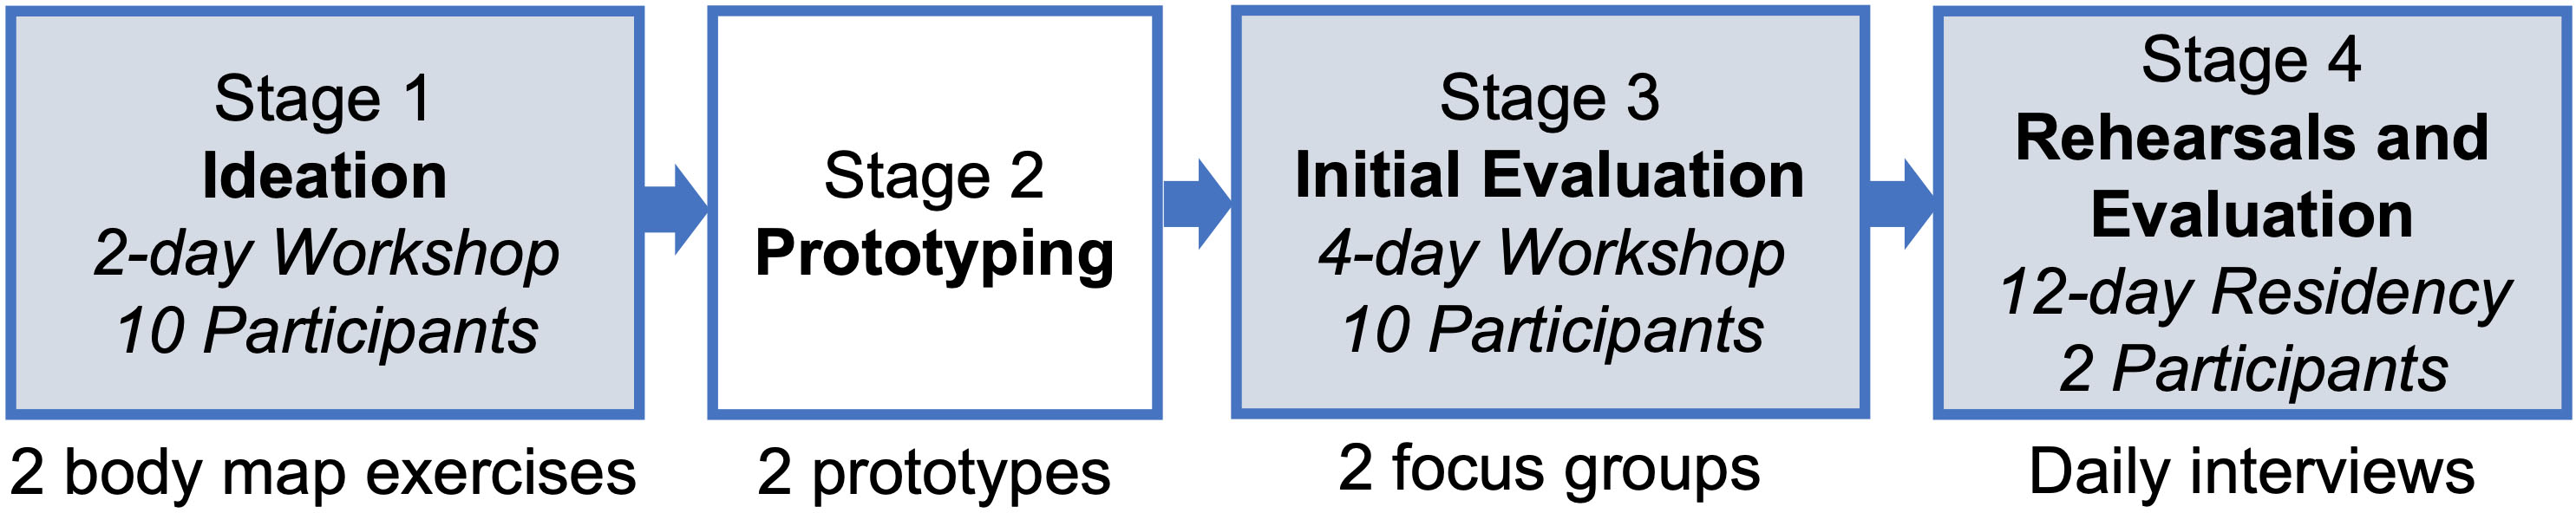
\includegraphics[width=0.9\linewidth]{Chapters/Figures/modi_dis/multistage.jpg}
  \caption{Diagram with stages of the research, over a six-month period}
    \label{fig:multistage}
\end{figure}
% Figure 1: Diagram with the four stages of the research, over a six-month period

\subsubsection{Data Collection and Analysis}

Movement exercises conducted in Stage 1 were video recorded and the respective biosignal data was collected (see Stage 1 section). We collected sketches from the dancers related to those exercises, using the two types of body maps identified in the Related Work section: \textit{free-form} and \textit{outline-based}. We asked dancers to annotate the body maps, following the approach by Gastaldo et al. \cite{gastaldo_body-map_2012}. These materials were scanned for use in the systems to be developed. Each dancer was asked to explain the body maps in their own worlds, to shed more light into the sketches – a body map \textit{testimonio}, using the terminology from Gastaldo et al.. The \textit{testimonios} were also video recorded.

In Stage 3, after the prototype development, we conducted two focus groups for the evaluation of both systems. In Stage 4, we conducted daily interviews with participants (across six days for each participant), for further evaluation and design iteration. These were audio recorded. The systematic data collection in Stage 4 is based on the technomethodology approach proposed by Dourish, involving the analysis of actions “moment-by-moment”, promoting a detailed analysis of actual practice \cite{dourish_where_2001} – adequate for the setting of choreography rehearsals. Therefore, we combined a shorter data collection and evaluation with more dancers (Stage 3), with a more extended and continuous evaluation, with fewer dancers (Stage 4).

The audio recordings of the two studies, in Stages 3 and 4 (focus groups and daily interviews, respectively), were transcribed and subjected to thematic analysis \cite{braun_using_2006}, independently. For each of the two thematic analyses, we coded the data using an inductive approach, and the codes were then organized into themes. We followed an inductive ‘bottom up’ approach to identify patterns within the data: “a process of coding the data without trying to fit it into a preexisting coding frame, or the researcher’s analytic preconceptions”. Therefore, in this process we were not driven by theory or the questions we asked. The analyses were conducted by the first author and cross-checked by the second. 

% We are aware that our profile as HCI researchers (particularly in the field of HCI) and also as artists ourselves may have influenced our interpretation of the data.  We used the software Atlas.ti (https://atlasti.com) to assist in the coding and analysis.

\subsubsection{Study Participants}

The two workshops involved a total of 12 international professional dancers in the field of contemporary dance, between 27 and 49 years old (11 female, 1 male), selected from an open call distributed to contemporary dance mailing lists (resulting in 92 applicants, 73 female, 19 male). 

Ten participants took part in the workshops on Stages 1 and 3. Two of the participants from Stage 1 could not attend the Stage 3 workshop due to scheduling issues, and were replaced by two other applicants from the initial open call. The two participants in Stage 4 (both female, 32 and 45 years old) were selected from the previous group of participants. The selection was based on a call for proposals, between Stages 3 and 4, targeting previous participants, to develop choreographies using the prototypes.

One reviewer of the corresponding publication critizised the gender imablance of the user group in respect to generizability. We may direct this to a higher number of female dance artists in the field of contemporary dance, and that the CVs of the male applicants were considered less fitted to the project than of the female applicants. It could even be commented that this effort actually poses to counter a historical overshadowing of non-male perspectives in Science and Technology Studies (STS) \cite{wajcman_feminist_2010,hook_soma_2019}.

\subsection{Design Stages}

\textcolor{red}{Move back to preliminary actions}
\subsubsection{Stage 1 - Sketching Workshop}

The first stage consisted of a two-day sketching workshop, which
took place at STL, a dance center in Tallinn, Estonia. The objective of this stage was to gather visual ideas and data about the dancers’ inner bodily processes during movement, to assist in the design and development of the interactive visuals systems for performance. Following approaches from our literature review, we used the two types of body maps identified (free-form and outline-based) as the main tool to collect visual ideas, and we used biosignal sensors to gather bodily data.

We decided to use biosignal sensors as one of the strategies toward our aim of revealing internal information from the dancer’s body. We used the BITalino R-IoT to acquire muscle activity, acceleration, and orientation data. The use of these sensing modalities is informed by the corresponding literature review, particularly in regards to stability and usablity during intense phyisical activity \cite{aly_appropriating_2021}.

The workshop involved three activities (the first on day 1, the other two on day 2):
\begin{enumerate}
    \item  The dancers prepared a movement exercise, consisting of five thematic sections, agreed upon collectively between them: Comfortable; Difficult; Undefinable; Aesthetic Form; and Open. Each dancer then created their own interpretation of the movement exercise, based on improvisation. This approach of combining improvisation with different, discrete, sections around a theme is similar (although smaller in scale) to the procedure followed by McDonald to generate an ML dataset for a dance piece \cite{mcdonald_dance_2018}.
    \item Each dancer was asked to perform the movement exercise, which was documented. The documentation consisted of video recordings and collection of biosignal data of each dancer. The data was labeled according to the dancer and to the section of movement exercise.
    \item The dancers drew body maps based on the movement exercise and their somatic impressions of it. We asked performers to create two types of drawings for each section of the choreography: free-form body maps and outline-based body maps (the two types of body maps identified in our Related Work section). We decided to have a range of more free-form and more constrained body maps in order to cover the different approaches identified in literature, and experiment with diverse designs for interactive visuals. Participants were given paper, colored felt pens and also clipboards for their drawings, so that they could move freely in the studio, and reenact the movements at will for accurate representation, while having the drawing materials at hand.
\end{enumerate}

The free-form body maps (figure \ref{fig:free-form-map}) resulted in very diverse and individual approaches. Each dancer produced five free-form body maps -- one per section. Following the approach by Gastaldo et al. \cite{gastaldo_body-map_2012}, we asked participants to annotate these body maps. In our case, the annotations were done in an overlay sheet, which was stapled to the main page for the drawing. That way, the drawings could be scanned independently of the annotations, in the future (e.g., for animation purposes). We also recorded video \textit{testimonios} of dancers explaining their body maps.

\begin{figure}[ht]
  \centering
  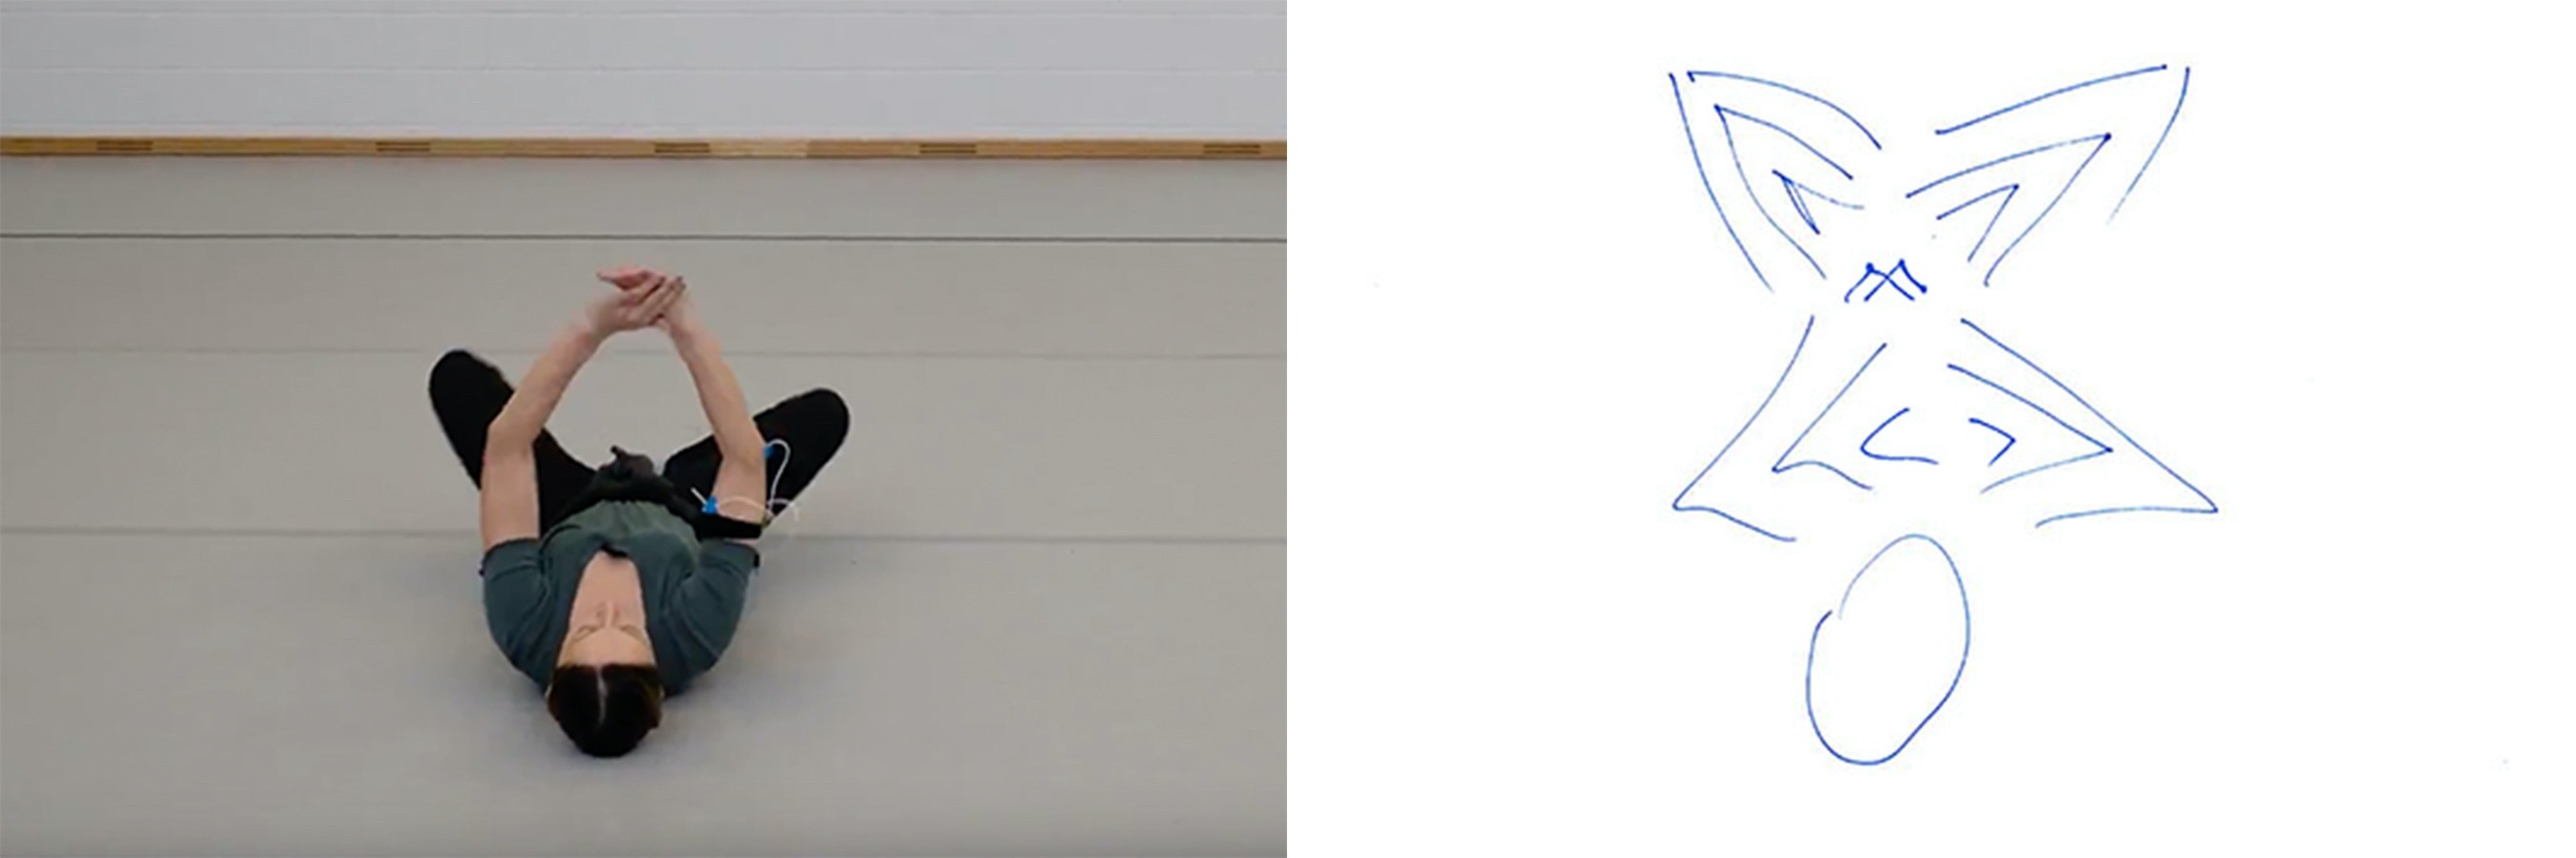
\includegraphics[width=0.9\linewidth]{Chapters/Figures/modi_dis/Zjana.jpg}
  \caption{Free-form body maps. Left: dancer executing a movement section. Right: free-form body map drawn by the same dancer corresponding to that movement section}
    \label{fig:free-form-map}
  %\Description{}
\end{figure}

The outline-based body maps (figure \ref{fig:outline-based-map})  were more constrained, and involved coloring the main body areas involved in that movement, as perceived by the participant (ten drawings per dancer – two per section of the choreography). The silhouette adopted was based on one of the outline-based body maps identified, used by  \cite{nummenmaa_bodily_2014}. Each drawing was labeled according to the specific section of the choreography that it corresponds to. A total of 150 body maps were produced (50 free-form and 100 outline-based body maps).

\begin{figure}[ht]
  \centering
  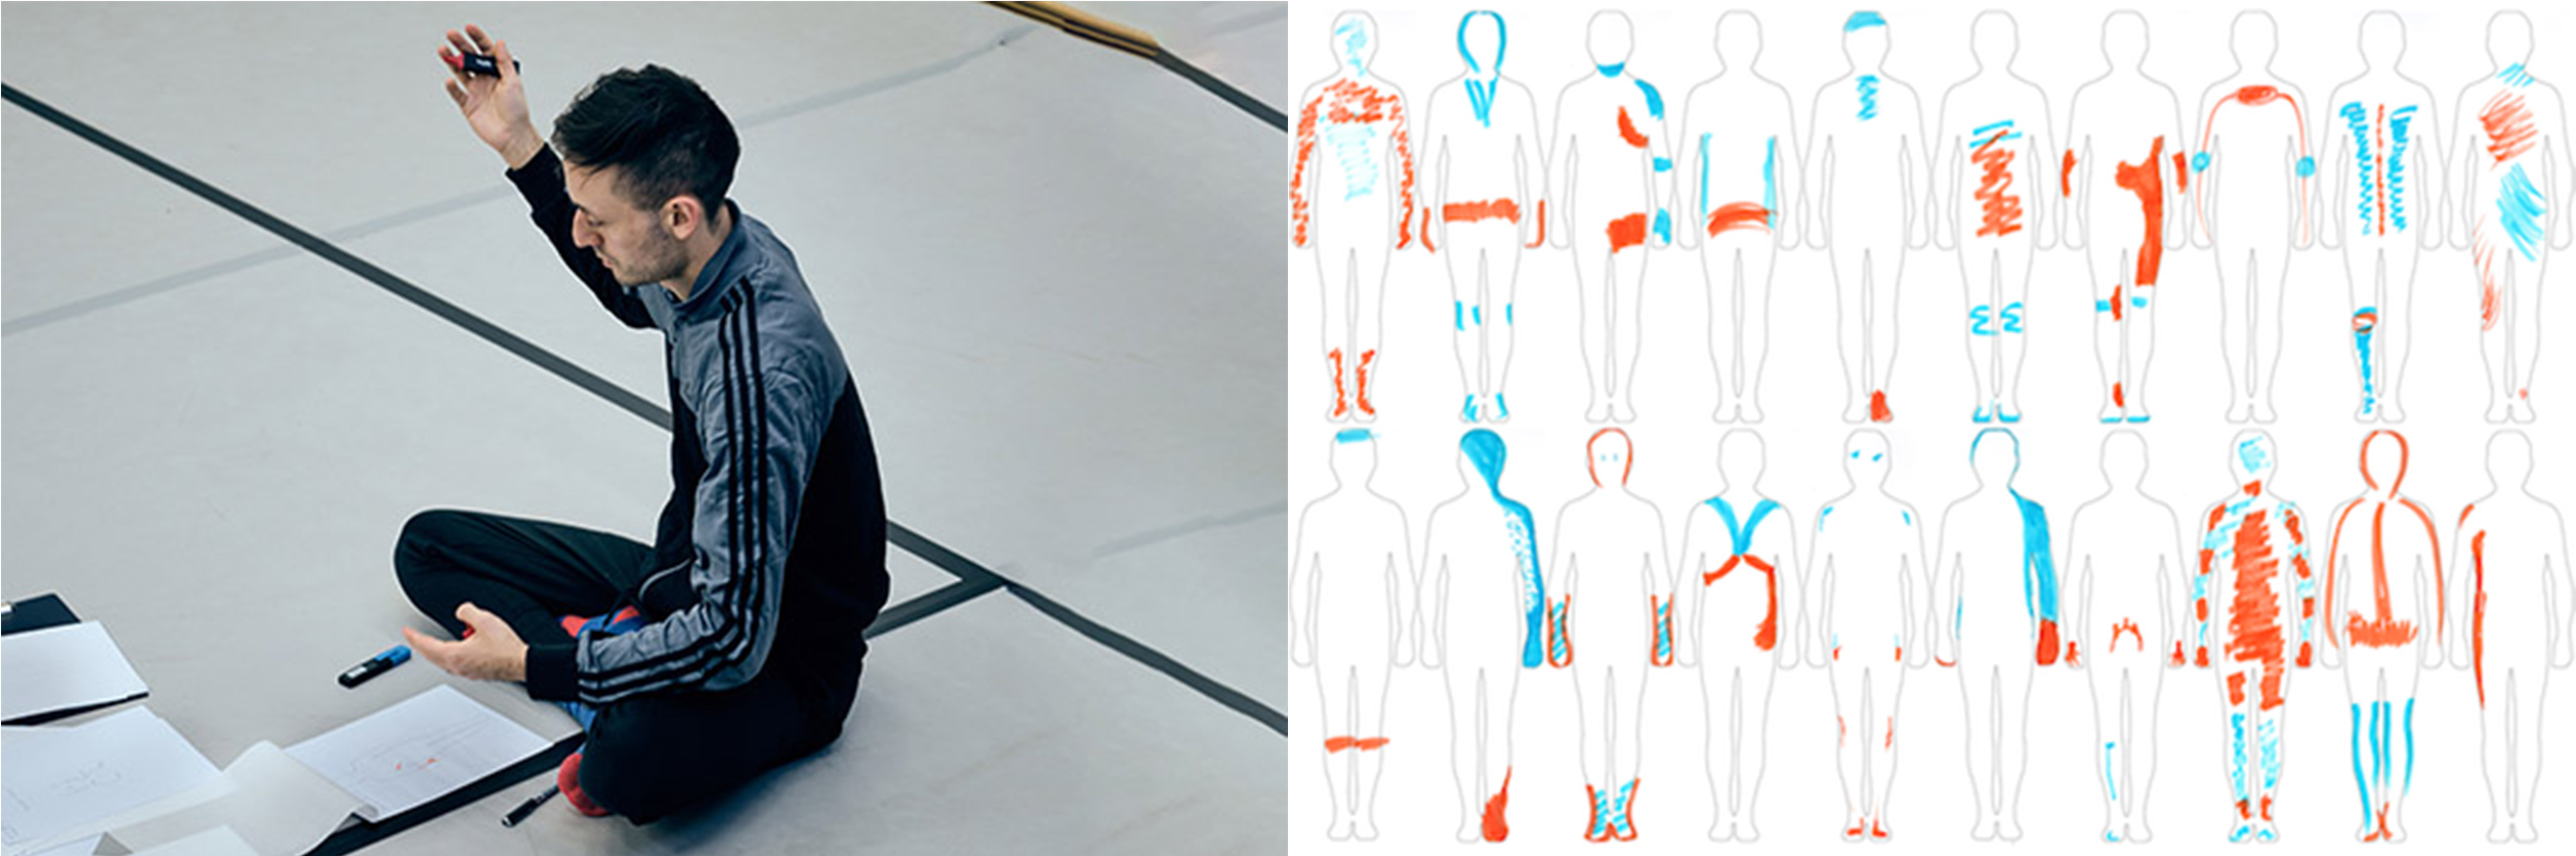
\includegraphics[width=0.9\linewidth]{Chapters/Figures/modi_dis/Juan.jpg}
  \caption{Outline-based body maps. Left: dancer partly reenacting a movement section while drawing an outline-based body map of that movement. Right: 20 of the total 100 outline-based body maps.}
    \label{fig:outline-based-map}
\end{figure}

\subsubsection{Stage 2 - Prototype development}

After the initial workshop, our research team set out to conceive approaches for interaction design and visualization, which would leverage the visual material created by dancers in Stage 1, informed by related literature. We aimed to generate motion graphics from drawings created by the performers. To fulfill that, we followed two different approaches, each considered more suited to outline-based or to free-form body maps, resulting in two prototypes.

\paragraph{Machine Learning Interactive Visuals Approach}

For the outline based body maps, we employed an approach we entitled Machine Learning Interactive Visuals (MLIV). Each body map was labeled according to a specific section of the choreography and then matched with the sensor data recorded, while the movement was being performed. We developed a MLIV system using TensorFlow (https: //www.tensorflow.org) \cite{abadi_tensorflow_2016}, capable of morphing between the performer’s body map drawings by predicting the interpolated frames, according to biosignal sensor data. The workflow is illustrated in figure \ref{fig:ml-model}. This is done through a Convolutional Autoencoder (CAE), an unsupervised model consisting of an encoder and decoder function. We adopted an autoencoder approach informed by Berman and James \cite{liapis_learning_2018}, who found that it was suited for live applications in dance. The encoder computes compressed representations of the images, assigned according to the visual features interpreted by the model, referred to as the latent vectors. To allow navigation between these vectors, the decoder is capable of generating continuous interpolations between the drawings, resulting in a series of new, reconstructed, images.

\begin{figure}[ht]
  \centering
  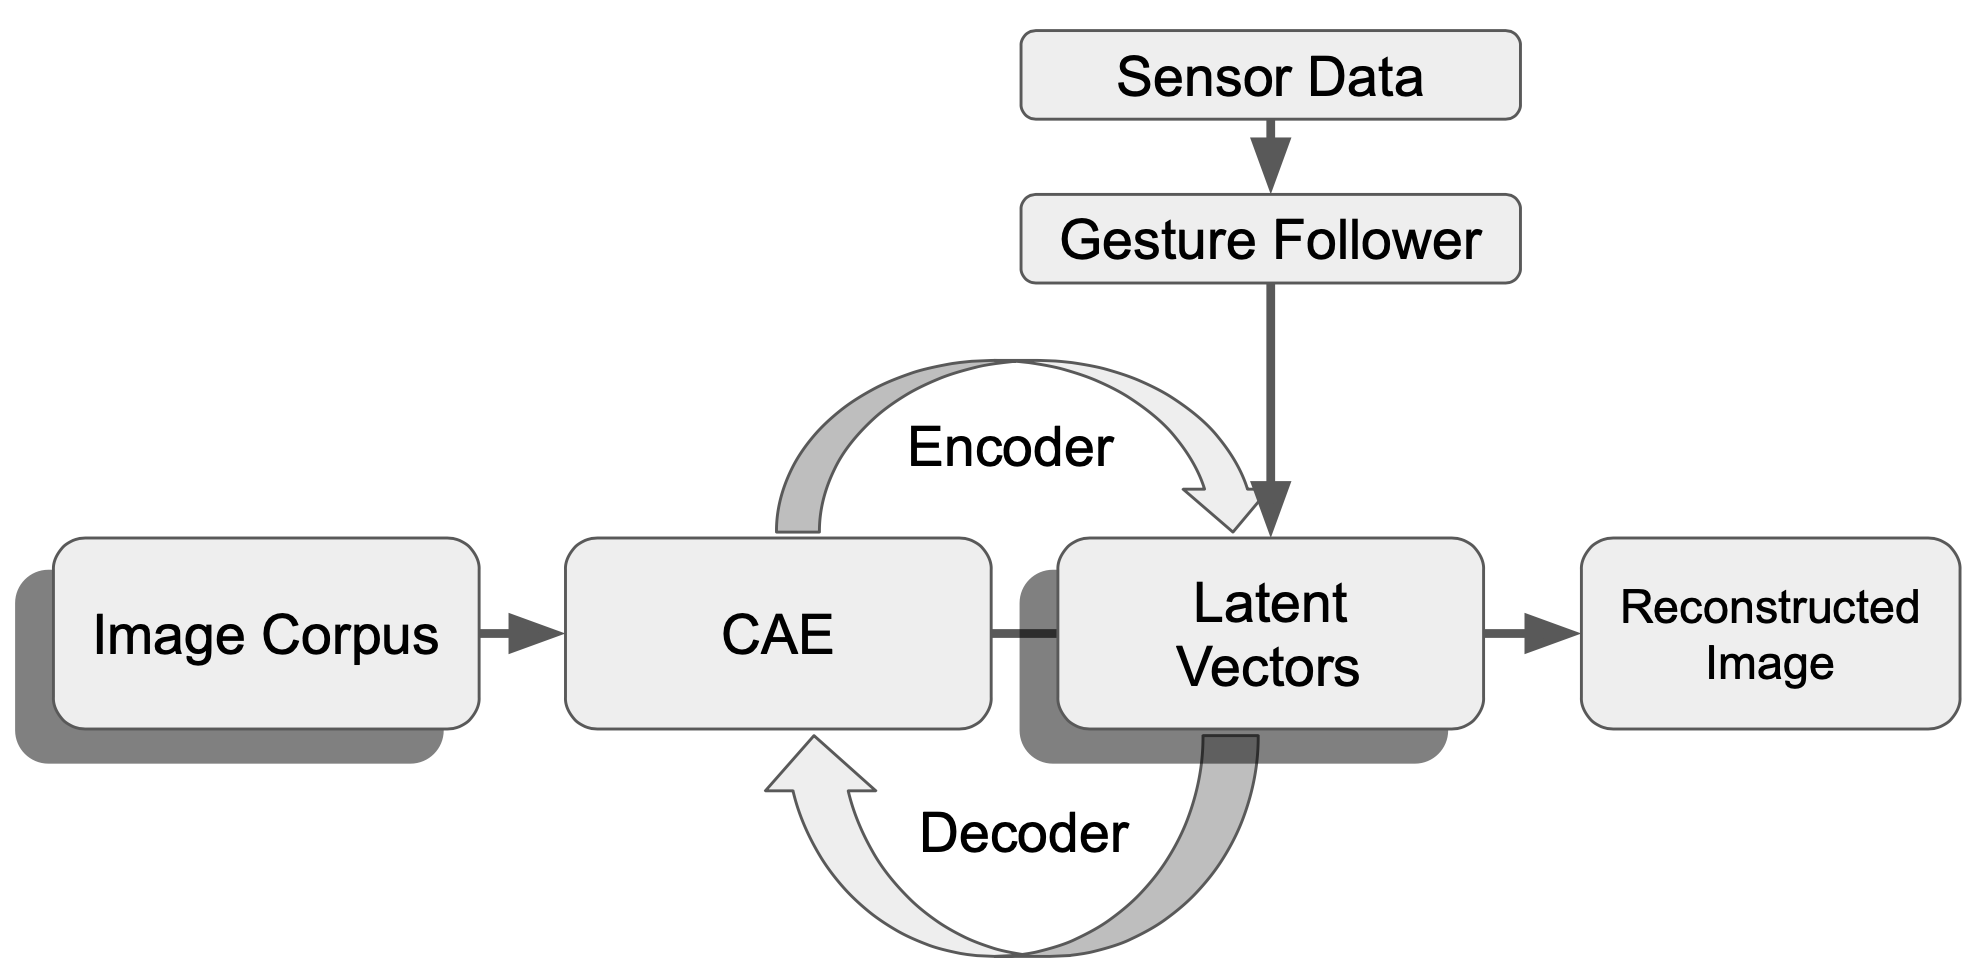
\includegraphics[width=0.9\linewidth]{Chapters/Figures/modi_dis/ml-model.png}
  \caption{MLIV design framework diagram, as followed in the respective prototype.}
    \label{fig:ml-model}
\end{figure}

To enable user interaction, we adopted a regression-based model, trained on a set of postural gestures from the performer, producing a continuous output while gestures are repeated and performed (detailed in Section X.X). We coupled the regression model with the incoming acceleration and electromyography sensor data captured from BITalino R-IoT. This orchestration allows the performers to manipulate the style and time-dynamics of the animation through movement (navigating around the latent vector space through movement).

This work led to the MLIV prototype. The system analyzes in real time the incoming sensor data from the dancer’s movement (figure \ref{fig:ml-screenshot}, first row). When fed into the gesture recognition layer, it tries to match the incoming sensor data with a segment form the pre-trained data corpus. It identifies the closest data segment match from the corpus, retrieves and adapts the body map corresponding to that movement segment (figure 5, second row). Following that, the process is repeated. When the next body map match is found, the system generates interpolated frames between the two matches (current and previous match), creating an animation (figure \ref{fig:ml-screenshot}, third row). The process then repeats again. This way, the system can generate in real time a vast number of possible animations based on the movement being executed, which would be unfeasible to generate manually.

\begin{figure}[ht]
  \centering
  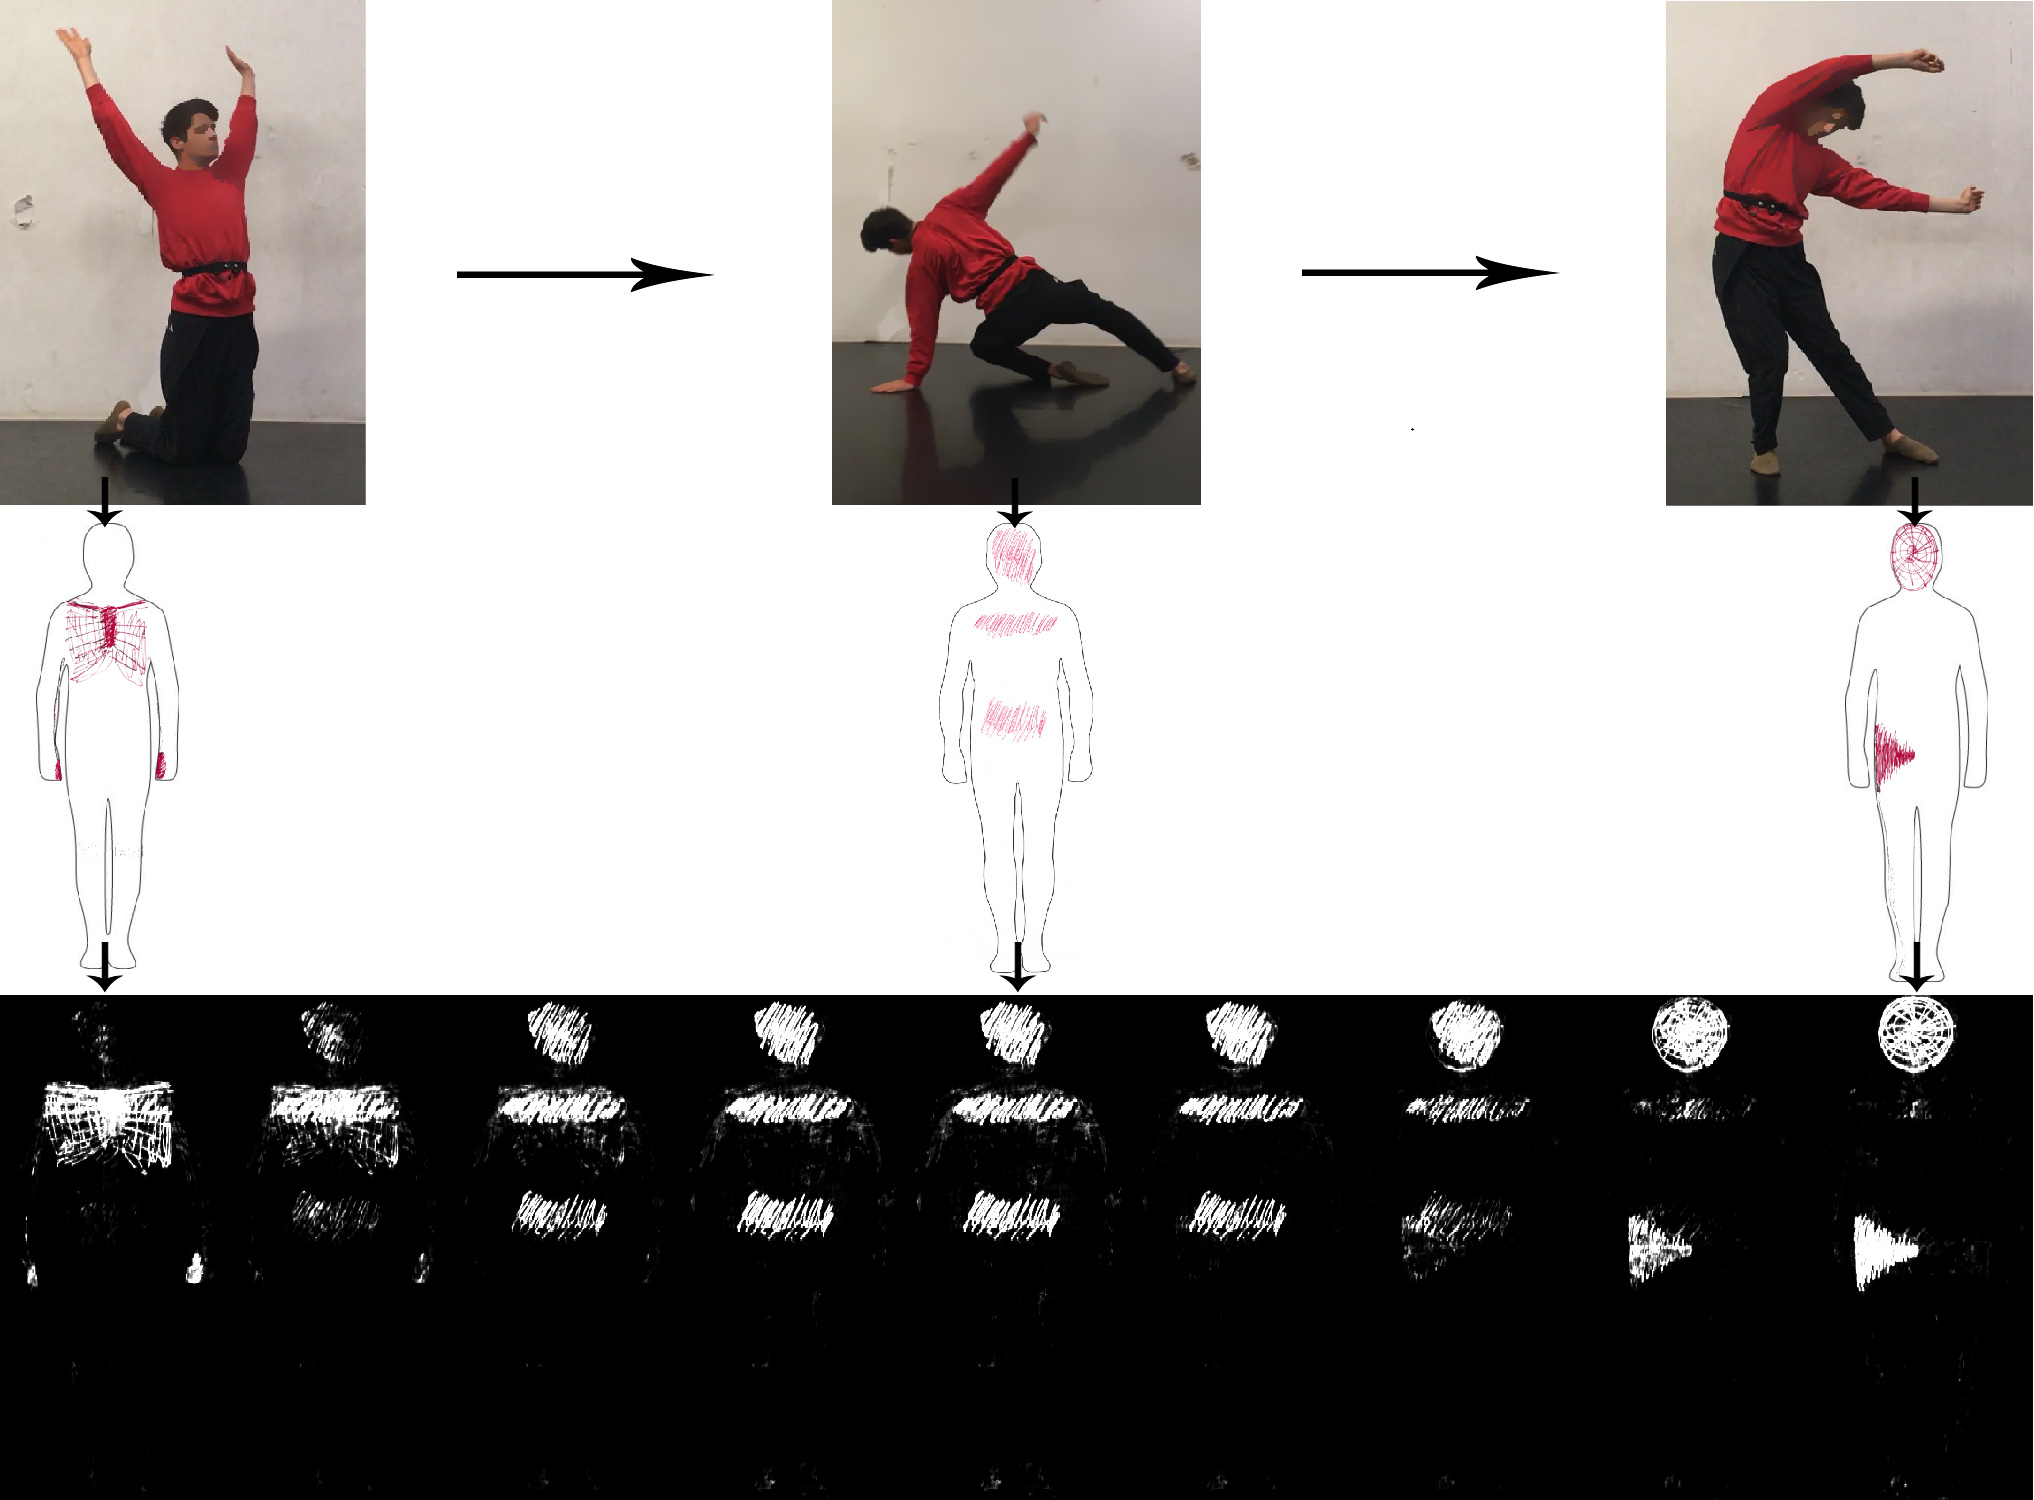
\includegraphics[width=\linewidth]{Chapters/Figures/modi_dis/sensor-drawing-3rows-large.png}
  \caption{Sequence of real time visualization frames from the MLIV prototype, based on movement and matching body maps.}
    \label{fig:ml-screenshot}
  %\Description{}
\end{figure}

% Figure Movement -Sketch - Output

% Figure 5: Sequence of real time visualization frames from the MLIV prototype, based on movement and matching body maps.

\paragraph{Composite Animation Interactive Visuals Approach}

We were aware that there would be difficulties using MLIV with the free-form body maps. Due to the relatively small number of drawings (50) and the diversity of visual features, there was a strong likelihood of overfitting – thus presuming our computational model (presented above) would not recognize meaningful patterns in the dataset. This was apparent during the initial prototyping phase, when feeding new inputs. We observed the inferred outputs would either resemble near replicas of the original data, or noisy representations, so incohernet, they held almost no association with any of the dancers’ visual intentions (i.e the original sketch).

\begin{figure}[ht]
  \centering
  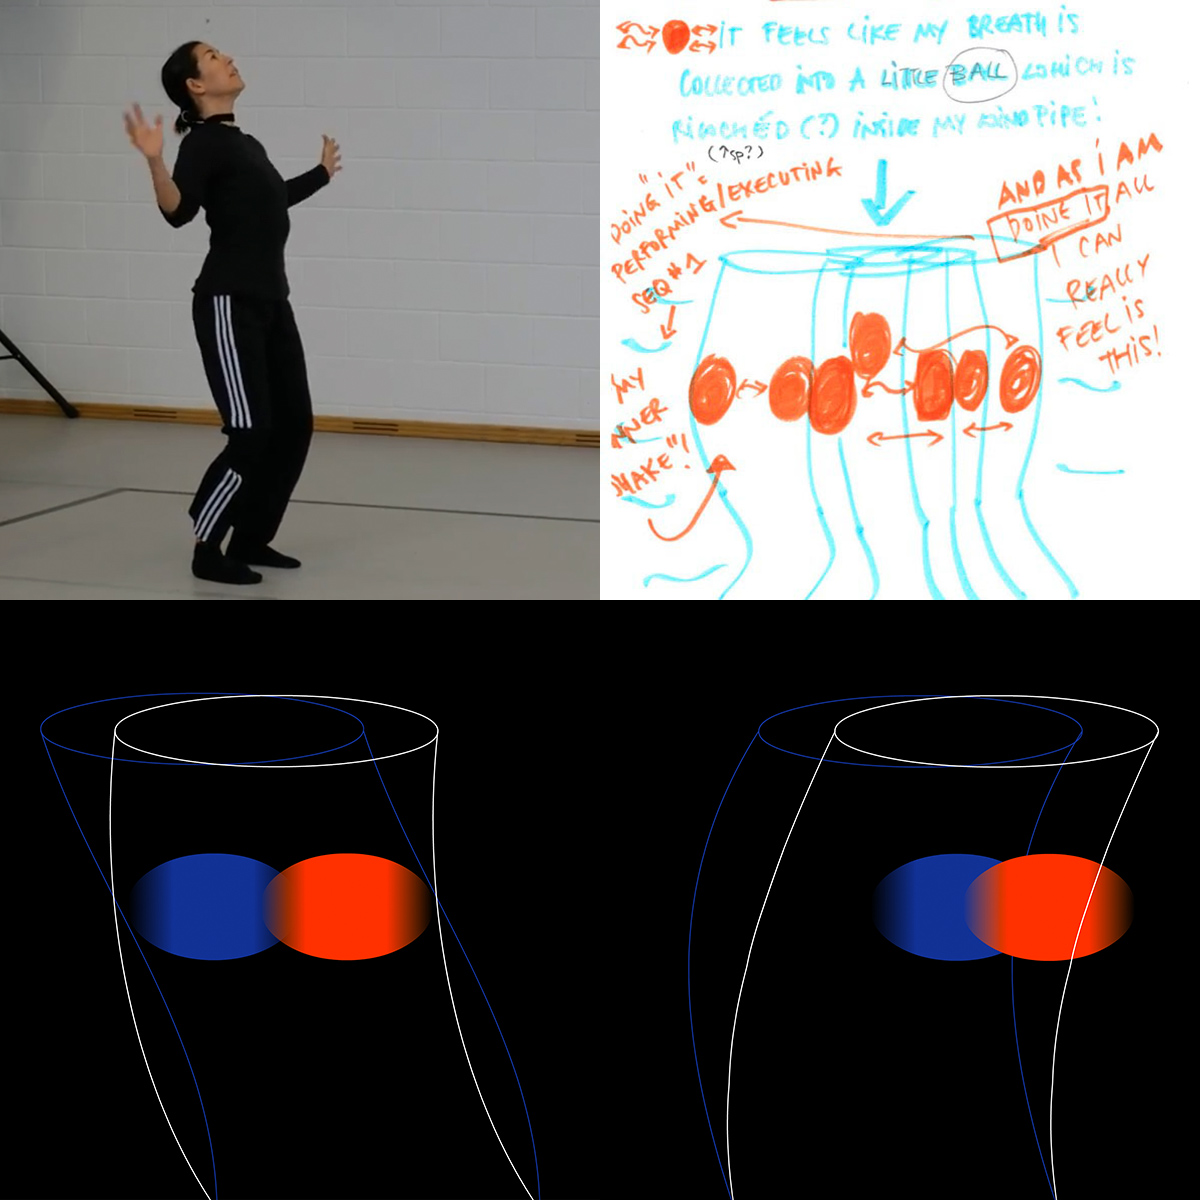
\includegraphics[width=0.65\linewidth]{Chapters/Figures/modi_dis/Stage1-animation.jpg}
  \caption{CAIV approach. Top left: dancer executing a movement section. Top right: the free-form body map drawn by the same dancer corresponding to that movement section, with annotations. Bottom: two frames of the motion graphics created by the animator, based on the documentation of the movement section, represented on top of the image.}
    \label{fig:Stage1-animation}
  %\Description{}
\end{figure}

Instead of MLIV, we adopted a ‘human learning’ approach we entitled Composite Animation Interactive Visuals (CAIV), to create interactive visuals from the free-form body maps. We use the term ‘composite animation’ to adapt the concept of composite drawings to animation. Composite drawings are used in forensic art and can be defined as freehand drawings, created by a forensic artist, combining various sources into a single graphic image \cite{stewart_forensic_2015}. These sources can be, for example, witness descriptions and CCTV footage related to a crime. To pursue this concept, we hired a professional illustrator and animator, André Carrilho, to transform the free-form body maps into motion graphics, also informed by the annotations on the body maps and the matching video sequence. With these elements, he created the different animations, in a way that respected the original body maps, while slightly simplifying and harmonizing the different animations (figure \ref{fig:Stage1-animation}). These slight simplifications and harmonizations aimed to allow for a better ‘mixing and matching’ of the animations during a performance. In this stage, the animator created ten motion graphics sequences, one per dancer (with the possibility to add more in the future) – chosen based on the potential of the respective body map for animation, while covering all five section themes. Our research team reviewed the animations as part of a ‘quality assurance’ process, to check if they conveyed the dancer’s materials well. In some cases, the animator fine-tuned the animations according to our suggestions.

\begin{figure}[ht]
  \centering
  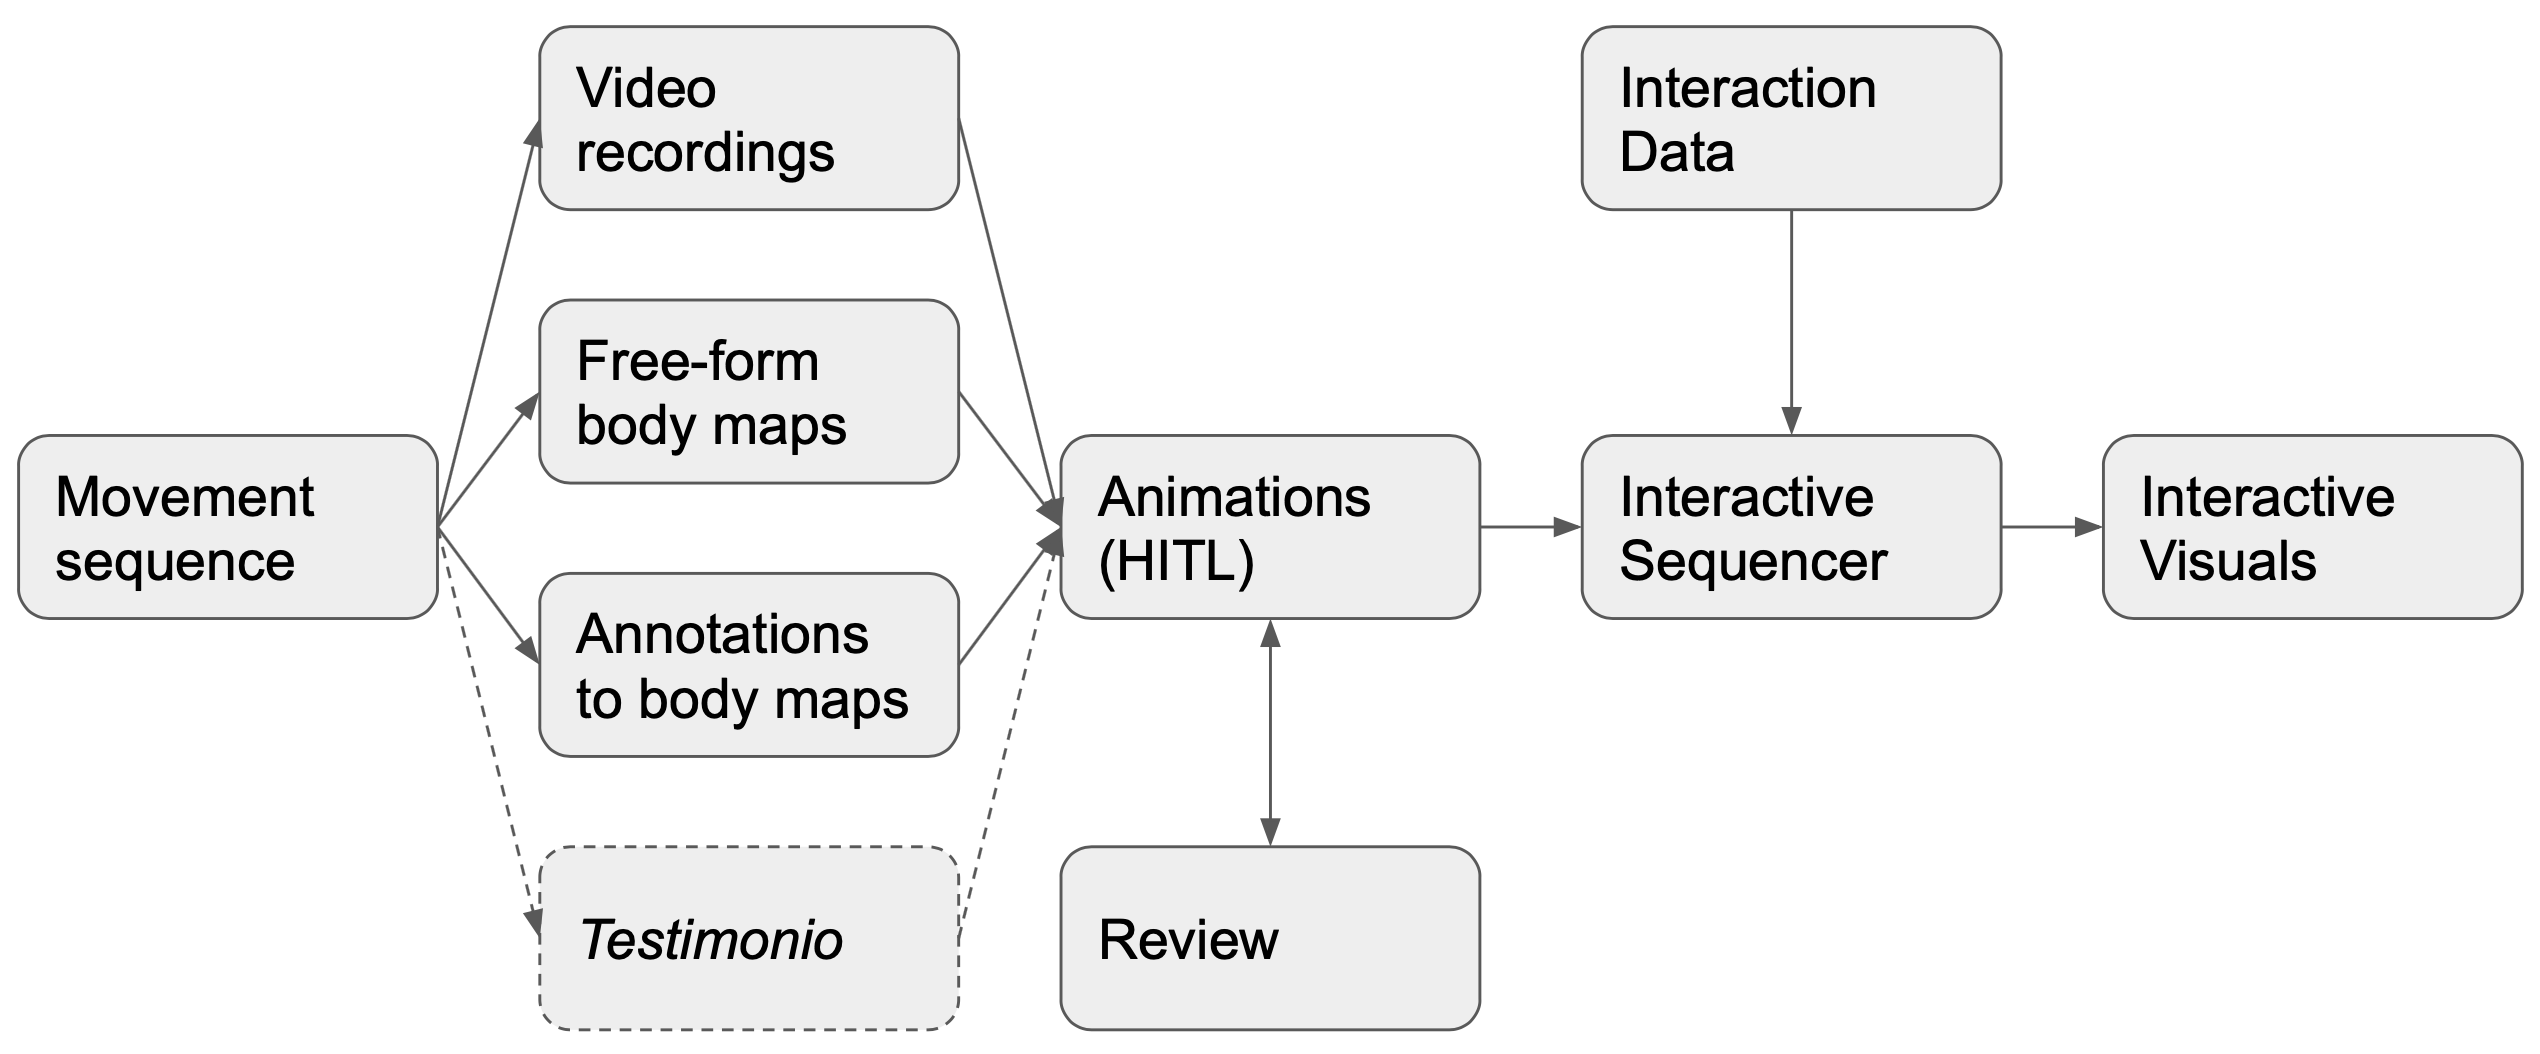
\includegraphics[width=0.7\linewidth]{Chapters/Figures/modi_dis/hitl-model.png}
  \caption{CAIV approach diagram, as followed in the respective prototype.}
    \label{fig:hitl-model}
  %\Description{}
\end{figure}

For the interaction design in our CAIV approach, we did not use ML or biosignal sensors, and focused on the non-linear sequencing of animations, in a way that would support flexible choreographic decisions. We created a visual sequencer for the animations using \textit{Isadora} (\url{https://troikatronix.com}), an “easy to use but also sophisticated software for both workshops as well as performance” \cite{delahunta_isadora_2005}. We designed a customizable Graphical User Interface (GUI) for the sequencer, to structure and trigger the animations non-linearly, onthe-fly. Figure \ref{fig:hitl-model}) shows the GUI coexistinging with video thumbnails, video preview and the data flow, allowing for spontaneous reconfiguration, while maintaining ease of use for the operator (e.g., the choreographer, the dancer or a technician).

The animations could be used, for example, as an onstage virtual ‘partner’ for the dancers (using Hsueh et al’s terminology \cite{hsueh_understanding_2019}) or as a ‘director’ (that could represent the choreographer, or another role). During the performance, it allows to display not just a single animation, but also multiple ones, as a ‘menu’ of options for the next animation (for example, visualizing the options for the next movement of a virtual entity, or the next instruction for the dancer to follow). As placeholders for animations, videos, images or text can be used. Our CAIV approach is modeled in figure \ref{fig:hitl-screenshot}.

\begin{figure}[ht]
  \centering
  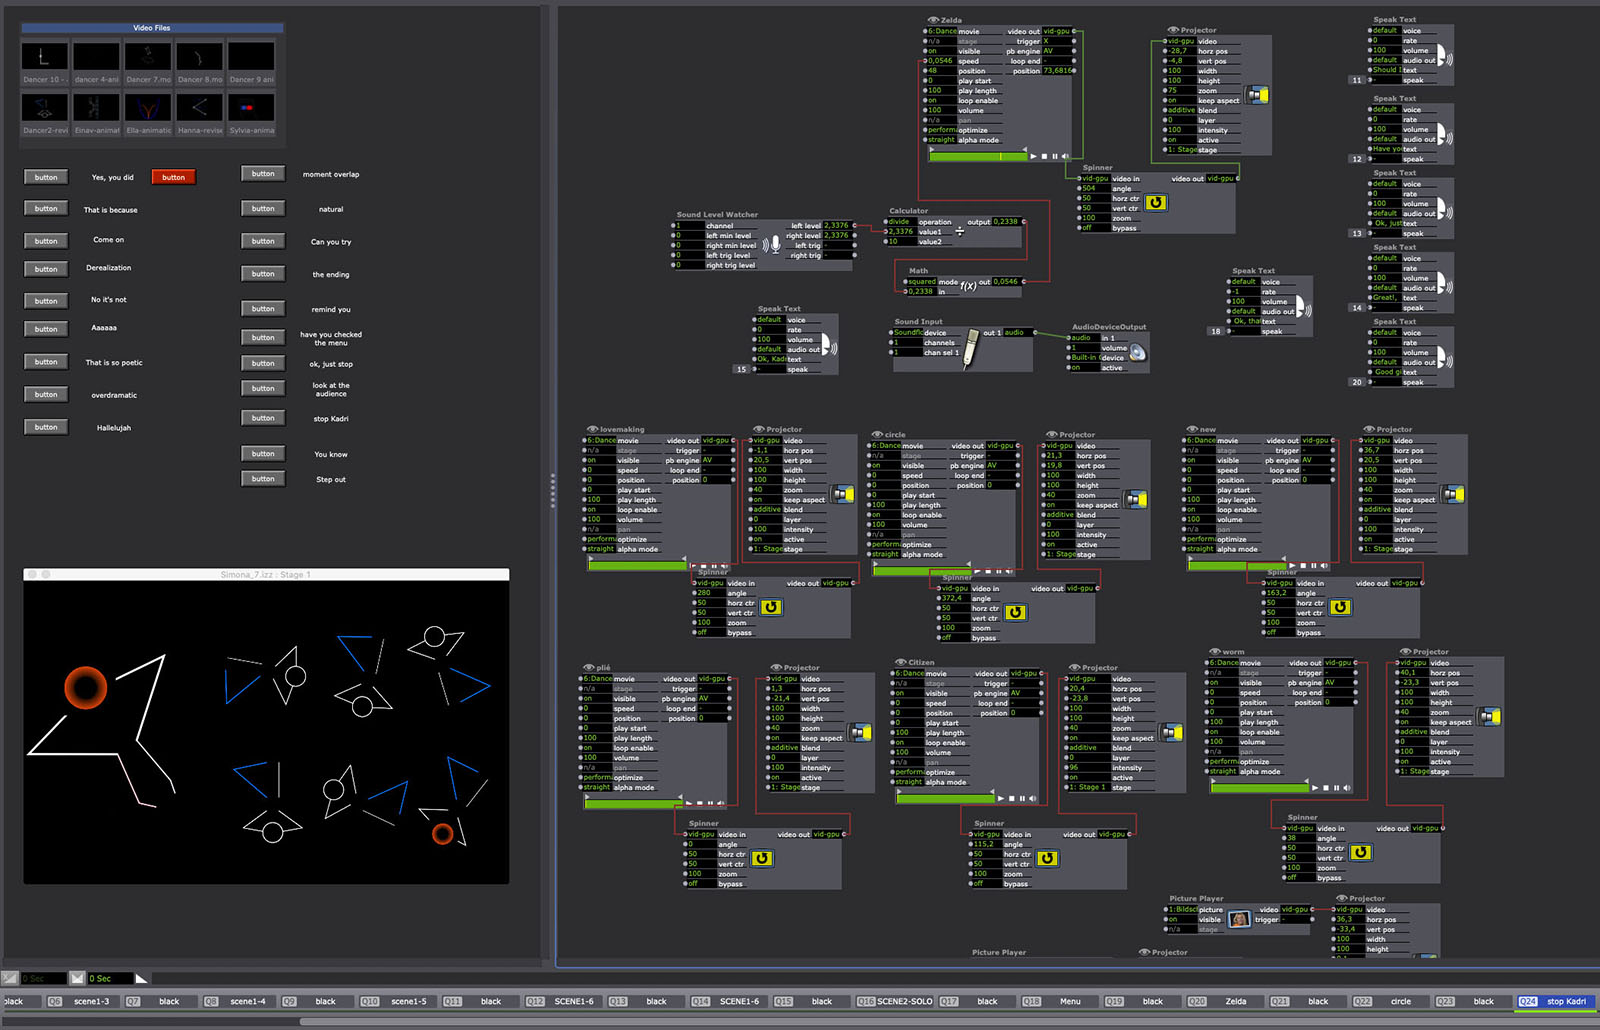
\includegraphics[width=0.65\linewidth]{Chapters/Figures/modi_dis/hitl-screenshot-s.jpg}
  \caption{CAIV prototype screenshot, as seen by the operator. Top left: animation thumbnails and GUI to trigger animations. Bottom left: preview of the visuals to be projected on stage (in this case, a image of the ‘menu’ of possible next animations in the sequence). Right: \textit{Isadora} data flow.}
    \label{fig:hitl-screenshot}
\end{figure}
% Figure 7: CAIV prototype screenshot, as seen by the opera- tor. Top left: animation thumbnails and GUI to trigger ani- mations. Bottom left: preview of the visuals to be projected on stage (in this case, a image of the ‘menu’ of possible next animations in the sequence). Right: Isadora data flow.

% Figure 8: CAIV approach diagram, as followed in the respec- tive prototype.

\subsection{Evaluation Stages}

\subsubsection{Stage 3 - Initial Evaluation Workshop and Results}

Stage 3 consisted of a four-day workshop, which took place at the Interactive Technologies Institute, Madeira, Portugal. The main objectives of this second workshop were to evaluate the prototypes and collect feedback, leading to their improvement. Ten performers attended the workshop – eight from the first event (two of the original participants could not attend), and two new performers (D5 and D10), recruited from applicants to the original call.
During the four days, the dancers freely tried out the prototypes, and gave us informal feedback, which we used to iterate on those prototypes on-the-fly. On the first day, after a general introduction to the prototypes, each participant was asked to choose one of the two prototypes, for more in-depth testing during the rest of the workshop. From then on, the dancers were organized into two groups of five participants: MLIV group, composed of D1-D5; and CAIV group, composed of D6-D10; focusing on the respective prototypes (figure \ref{fig:tests}). On the last day, we organized two focus groups (one with each group of participants), aiming to give feedback to the respective prototype. In the focus group sessions, participants were asked to convey their impressions of the prototypes, and were prompted to mention positive and negative aspects. The two sessions had a duration of approximately one hour each. The transcriptions of the two focus groups were subjected to thematic analysis (as presented in the Methods section), resulting in four common themes: introspective visualization; affordances as inspiration and instructor; communication with audience; and openness and modularity.

\begin{figure}[ht]
  \centering
\hspace{8em}
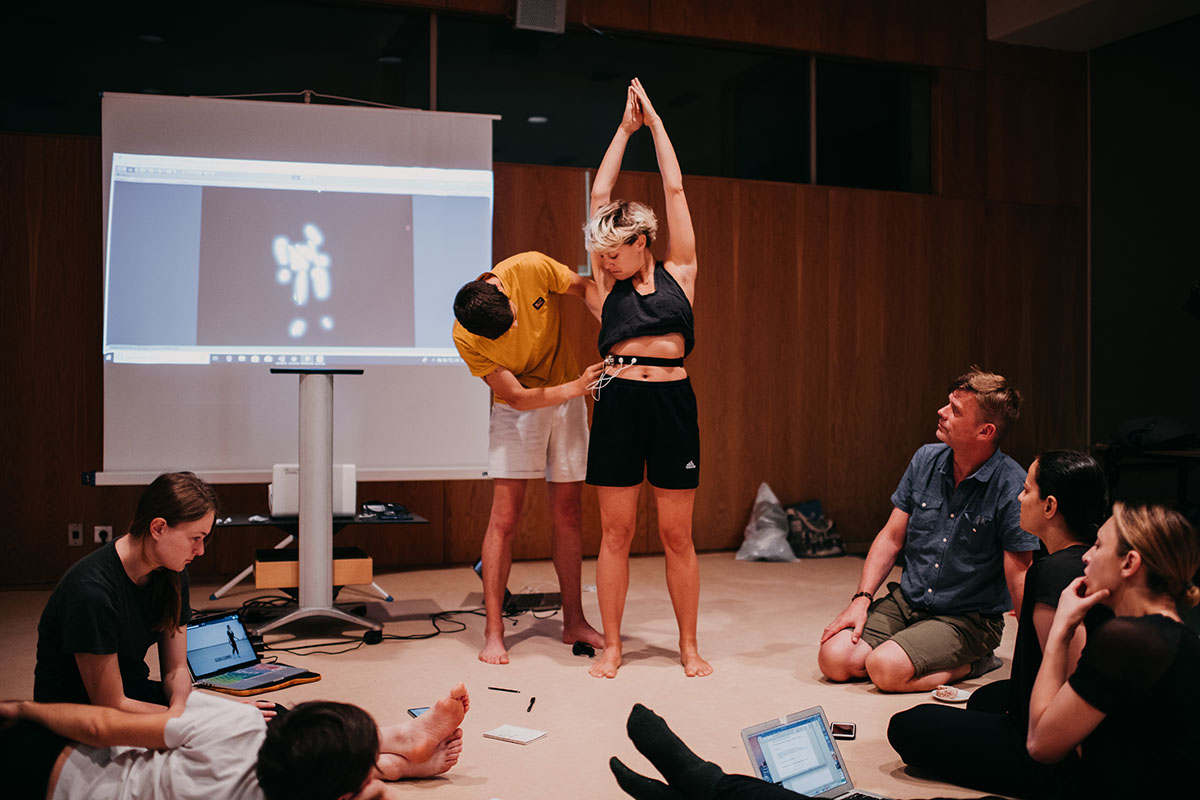
\includegraphics[width=0.7\linewidth]{Chapters/Figures/modi_dis/ml-test-s.jpg}
\hspace{-12em}
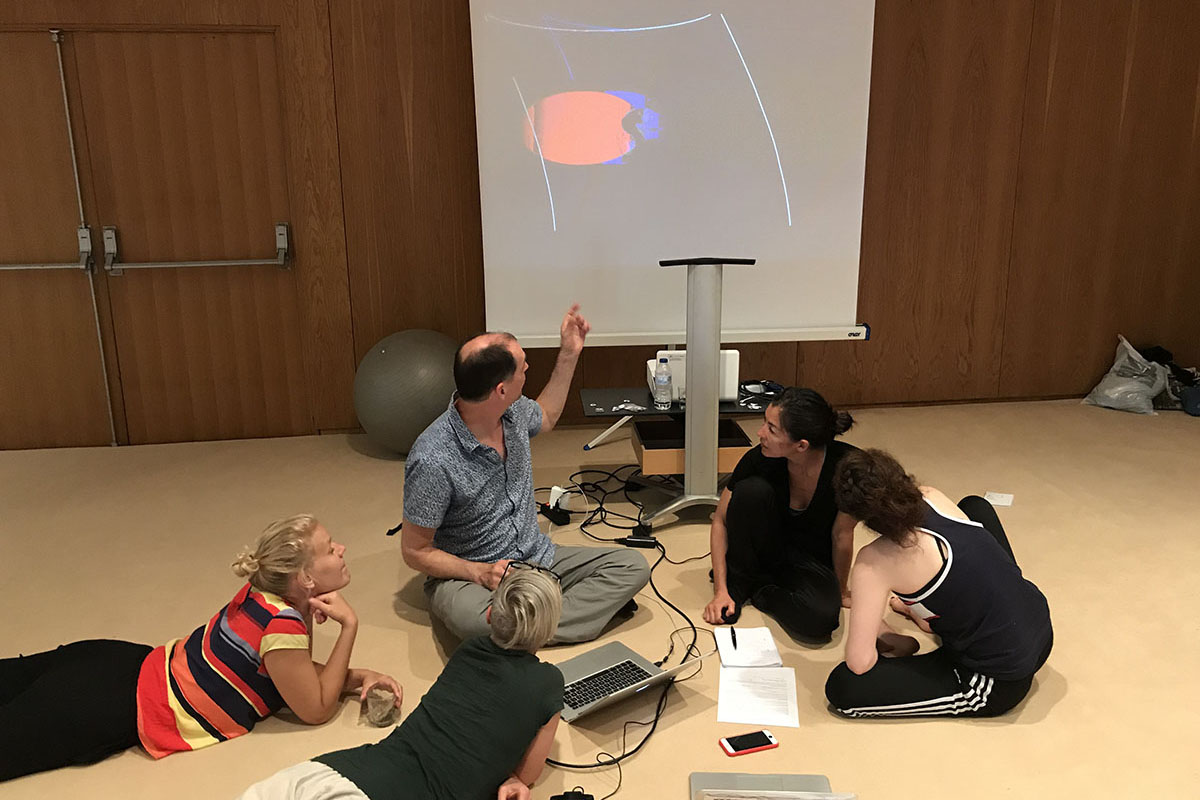
\includegraphics[width=0.7\linewidth]{Chapters/Figures/modi_dis/hitl-test-s.jpeg}
\caption{Initial prototype evaluation. Top: MLIV group. Bottom: CAIV group.}
\label{fig:tests}
\end{figure}

% Figure 9: Initial prototype evaluation. Left: MLIV group. Right: CAIV group.

\paragraph{Introspective Visualisation.}

\textbf{MLIV group:} All participants mentioned they appreciated the capability of the MLIV prototype to visualize the subjective and introspective aspects of the body, as exemplified in the following statements:

\begin{center}
\begin{tabular}{ p{13cm}}
\textit{It takes your internal experience, this subjectively live body experience and puts it outside. (D1)
[The researchers] included our initial perspectives in order to develop this prototype, not just the movement, not just the shapes of movement, but also the introspective aspect of how you feel concerning movement. (D2)}
\end{tabular}
\end{center}

Although some participants enjoyed that the MLIV prototype took their sketches as a starting point: “It provokes the imagery according to our own notation” (D2), others considered the visuals monotonous (D3, D5). \textcolor{red}{include quote also}

\begin{center}
\begin{tabular}{ p{13cm}}
\textit{it was already like this anthropomorphic thing was very dominant already from the exercise there. And I agree, for me it was a very... the aesthetic of this output and the human form, for me it was very limiting while using it}
\end{tabular}
\end{center}

\textbf{CAIV group:} D9 enjoyed the capability to visualize the dancer’s decision process in the CAIV prototype: “We are revealing things that happened in the dancer’s head while we are dancing (...) to reveal this process that we are doing, actually most of the time unconsciously. Deciding. What is next? ”

\paragraph{Affordances as Inspiration and Instructor.}

\textbf{MLIV group:} Participants enjoyed the bodily data affordances of the MLIV prototype (D1, D3, D4), which changed their behavior: “It puts me in a state of not doing form, because it’s not a camera, but it puts me in a state of exploring, like, weird internal stuff that I don’t usually do” (D3). All participants considered using sensors to be inspiring for movement. As D2 stated: “It opens a lot my imagination of how to interact with a system, and what the system reads in me, and what it incorporates in my somehow subjective feelings toward my own movements”. Participants mostly disliked the slow reactivity of the MLIV prototype (D2, D5), although this was considered adequate by D1: “it takes a bit of time to see, which is how I deal with my dance practice”.

\textbf{CAIV group:} The dancers valued the non-linear flow of the CAIV prototype. A possible scenario that was identified is the system providing instructions to the dancer: “I think of a live situation where the dancer is kind of a slave of this big king of dance who’s sending me here and there. And I think it could be interesting because the performance would be different every time” (D10). Two dancers (D6 and D10) suggest using randomness to select the next steps in the sequence, instead of an interactive selection.
5.1.3 Communication with Audience. 

\textbf{MLIV group:} Participants recognized potential for communication between dancer and audience in the MLIV prototype: “I can make it clear enough the relationship between my movement and what the audience sees” (D2).

\textbf{CAIV group:} D7 identified potential in the CAIV prototype to make the audience move, using the system to output instructions for that movement. Related to this logic, D6 identifies pedagogical potential in the prototype, as a teaching and learning dance tool, suggesting adapting it to an interactive installation.

\paragraph{Openness and Modularity. }

\textbf{MLIV group: }D2 felt involved in the co-design process of creating the MLIV prototype: “It’s also a tool that we somehow coded, like participating in the process of coding”. Dancers wished to combine the prototype with motion capture (D2) and other types of sensors (D1). The wish for modularity was summarized by D4: “I am also more interested in trying out different possibilities, what are the possibilities where I can take the input from, which are the possibilities for the output” (an opinion echoed by D3).

\textbf{CAIV group:} The CAIV prototype showed potential as a tool to build choreography (D6, D7, D9), characterized as: “An open structure, which can be put down and rebuilt in a different way” (D9). However, it can be laborious, due to the need to prepare visual materials (D7, D10). Participants wished for a modular structure for it, combining features and functionalities taken from the MLIV prototype, such as: to add sensors (D7, D9) or ML (D7, D10)

\subsubsection{Stage 4 - Rehearsals of Choreographies and Evaluation Results}

After the Stage 3 workshop, participants could submit proposals for choreographies to be developed in the scope of [anonymized project]. Eight participants in the previous workshops submitted proposals, and four were chosen by the research team, based on the quality of the artistic concept, innovative approach and feasibility. Two of the selected proposals included the use of the MLIV and CAIV prototypes. For the scope of this paper, we focus on the work developing the two respective choreographies. The two participants (authors of the proposals) will now be referred to as ‘choreographers’, to reflect their change of role. The choreographer using MLIV will be referred to as C1, and the one using CAIV will be referred to as C2.  

C1’s proposal text was aligned with our aim of exposing non-visible elements:

\begin{center}
\begin{tabular}{ p{13cm}}
    \textit{In augmenting the interior realities through explorations of imaginary, sensations, creative fantasy, and the inner body-textures of the dancers relative to the exterior world (spectator), I seek to demonstrate unusual characteristics of dancing by creating a (visual) menu consisting of unusual perspectives of a dancing Body}
\end{tabular}
\end{center}

C2’s proposal was equally in line with our aim, focusing on the thinking and choice processes of the dance artist. It stated:

\begin{center} 
\begin{tabular}{ p{13cm}}
    \textit{I want to give the audience an insight on dance making, by showing the invisible process behind the choices one makes when creating a piece. (...) The audience will perceive 2 types of presentations: a human one and a virtual one. (…) Its proposals [of the virtual entity] would materialize in Animated Drawing, that envision its own movements, accompanied by related poetical explanations.}
\end{tabular}
\end{center}

Meanwhile, we made improvements to the prototypes, to address limitations identified in Stage 3. In the MLIV prototype, we introduced the wearable form-factor for the \textit{BITalino R-IoT}, with the sensory components embedded into a wearable enclosure; this reduced the noise in the signal during rapid movements, while allowing for faster setup times. In the CAIV prototype, we added new GUI elements in \textit{Isadora} for ease of operation, this fine-tuning of the GUI continued also during the residency according to the needs of C2. The animator was commissioned to develop ten more composite animations, defined with C2.

In Stage 4, we organized a 12-day artistic residency with the selected participants. The residency took place in the [anonymized] performance space. The objective was to develop each choreography and rehearse it, while continuously evaluating and fine-tuning the respective prototypes. It was intended to be more in-depth than previous workshops: it had fewer participants, and a longer duration, suitable for the rehearsal of a short choreography, building upon previous work. Choreographers were given the chance to work with local dancers (C1 chose two dancers, and C2 picked one). 

We arranged six separate six-hour studio sessions with each choreographer, across the 12 days, in alternating days (figure \ref{fig:rehearsals}). At the end of each session, we conducted short semi-structured interviews (six in total for each choreographer). We asked questions related to the use of interactive and visualization technology and the development of the respective project. The transcriptions of the interviews were subjected to thematic analysis (as presented in the Methods section), resulting in three common themes (body visualization aesthetics; feedback loops and connections; workflow and workarounds).  

\begin{figure}[ht]
  \centering
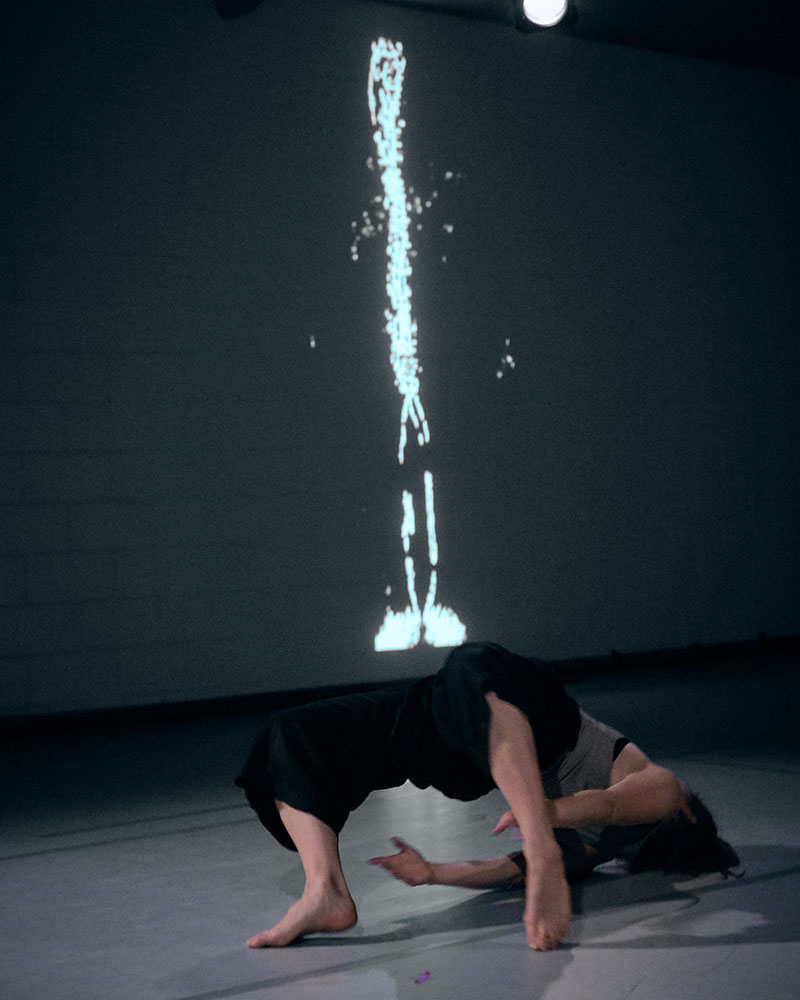
\includegraphics[width=0.475\linewidth]{Chapters/Figures/modi_dis/Sylvia.jpg}
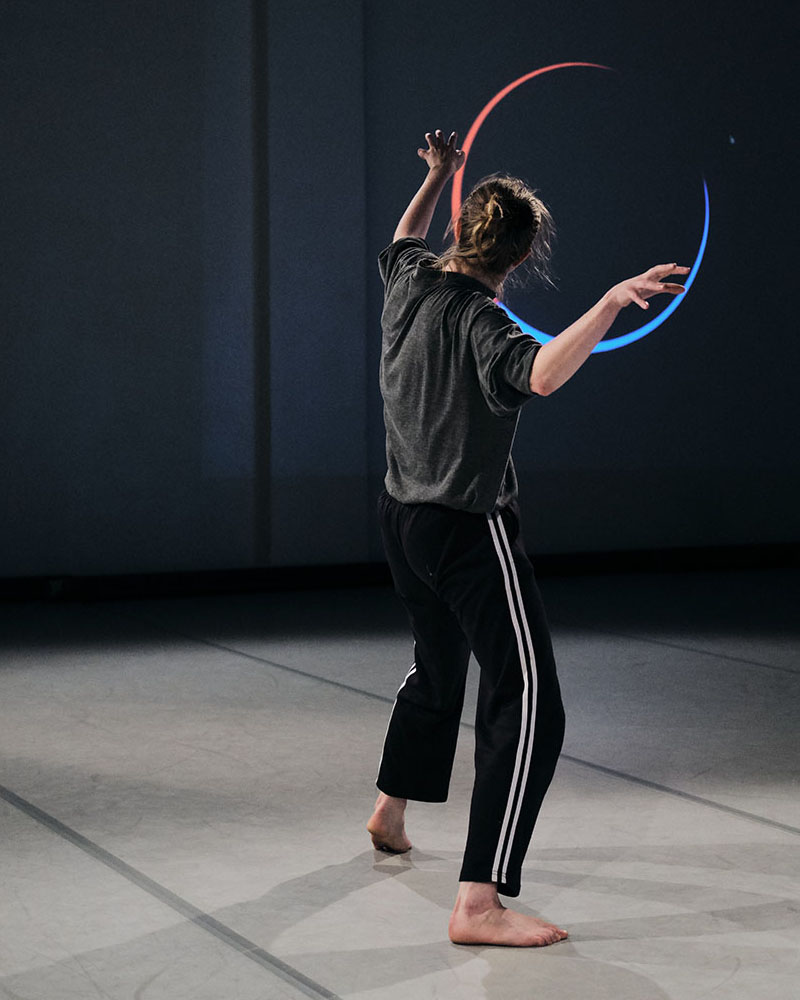
\includegraphics[width=0.475\linewidth]{Chapters/Figures/modi_dis/Kadri.jpg}
\caption{Images from the residency rehearsals. Left: MLIV approach. Right: CAIV approach.}
\label{fig:rehearsals}
%\Description{}
\end{figure}

\subsubsection{Body Visualization Aesthetics}

C1 enjoyed how the MLIV prototype facilitated visualizing biosignal data: “\textit{It's nice to be able to  see how biological information through the human body can affect or create [visual] effects}” (day 1). In particular, she felt that its pulsating aesthetics  highlighted the physiological side of the dancer: “\textit{It gives the breathing element. It shows the humans a little bit more delicate. It simulates organs, the idea of breath}” (day 3).

C2 used the animations in the CAIV prototype to simulate an artificial entity: “\textit{This visual means the body of another entity in a way}” (day 4). She enjoyed the minimal animations, representing the body of this entity: “\textit{I like [anonymized animator’s] drawing very much, I think we will get to a very beautiful action, a minimal kind of body}” (day 6).

\subsubsection{Feedback Loops and Connections}

C1 used the MLIV prototype to create a feedback loop between dancer and visuals, where the dancer influenced the visuals through the sensors, and the projected visuals in turn influenced the dancer: “\textit{a looping system, biological, digital, back to biology}” (day 1). To find that feedback loop, she explored different movements and system settings, “\textit{Trying to find the right kind of feedback that can trigger a movement or generate movement that's still justifiable in contemporary dance}” (day 1). By day 4, she felt “\textit{It did generate new movement, at least new possibilities for movement}”.

C2 wished to have a “\textit{dialogue}” with the dancer, by interacting herself with the visuals, through the CAIV prototype (day 1). With this system, she felt that she is connecting visuals and dancer: “\textit{I'm creating connections between image and body}” (day 4). By the end of the residency (day 6), she felt that the operator role is very efficient: “\textit{I liked that I could interact with [the dancer] in real time}”.

\subsubsection{Workflow and Workarounds}

C1 recorded and edited a large number of visuals generated during rehearsals, which she used to create a balance with interactive moments that she could not control, due to slow responsiveness of the MLIV prototype: “The film was something I could control, which was a nice balance with everything i could not control. Which was the live situation” (day 6).

C2 considered that the CAIV prototype was a quick tool in setting up the animations and visuals in the software, despite the laborious aspect of the prototype identified in Stage 3: 
“\textit{I think it's very good to work like this, really have a software that helps you create this structure, because it's about scoring and structuring in real time, and being able to make modifications in real time}” (day 3). On the final day (day 6) of the residency, in reference to our system, C2 stated “\textit{I have discovered this very efficient tool of structuring material very very fast}”. This allowed C2 to overcome the short time for developing the choreography: “Five days is not a good time for research. Meaning we need more time” (day 6, last day, in reference to the five previous days).

\subsection{Discussion}

We developed two design approaches to create interactive visuals for dance, based on machine learning and composite animations (MLIV and CAIV). Both rely on body maps drawn by dancers, based on their somaesthetic impressions. We first discuss aspects related to each of our two approaches, and then more generic aspects.

\subsubsection{Organic and Introspective Interactive Visuals, Machine Learning Approach}

The MLIV prototype was considered successful as a tool for revealing internal bodily processes, by the five dancers that evaluated it in Stage 3. Dancers appreciated that visuals took their own “notation” (D2) from their body maps as a starting point. C1 used the system for a longer time in Stage 4, and described the aesthetics of the system in more detail, showing a deeper understanding of its design, namely its organic and breathing-like visual affordances. On the interaction side, dancers in Stage 3 highlighted the impact that the system had in their own movement and even in their imagination (D2). In Stage 4, C1 explored this to create a feedback “looping system” between the biological, the digital, and back to the biological. She felt she achieved “new possibilities for movement”. We believe our MLIV approach complements related ML and movement approaches, such as \cite{murray-browne_latent_2021,silang_maranan_designing_2014}. These focus on other aspects of the movement data (flexible mapping and data classification), while our system focuses on visualization of inner aspects of the body.

\subsubsection{Accounting for Slow Responsiveness in Latent Steps}

The MLIV prototype had limitations in terms of responsiveness, which can be attributed to a small corpus of body maps (only 100) and limited sensor data collected. We applied a low-pass filter to the frame interpolation layer to compensate for identified abrupt jitters. However, this resulted in slower reactivity, both in terms of latency and slowness of the visualisation, relatively to the corresponding movements. This slow reactivity was considered by some dancers to be problematic in account of their first impression taken during Stage 3. To mitigate the risks of a slow responsiveness of the system in a performance, C1 combined real time visuals from the MLIV prototype with pre-recorded videos of visuals from rehearsals. We hypothesise that adding more drawings to the corpus, and collecting more matching data from the moment (potentially, with added sensors) could improve this responsiveness.

\subsubsection{Connecting Idiosyncratic Visuals with Movement, Composite Animation Approach}

Due to the more idiosyncratic nature of the free-form body maps, a different approach based on composite animations was pursued. To add interactivity to the resulting animations, we developed a dedicated system with Isadora, the CAIV prototype. The resulting animations were considered aesthetically successful by C2, and she enjoyed their minimalism. She used the animations to represent the body of an artificial entity that would enter a dialogue with the dancer. C2 controlled this artificial entity herself, by operating the CAIV prototype. This way, she could interact with the dancer in real time, which she enjoyed. The animations, grounded on dancers’ movement and related somaesthetic impressions, together with the sequencing system, allowed her “creating connections between image and body” (C2). The sequencing system for the animations was also considered successful in terms of visualizing inner processes. This relates to the proposal of revealing a movement decision process realized in our preliminary focus group \cite{masu_how_2019}. In the initial evaluation, D9 stated that the CAIV prototype had the potential for “revealing things that happened in the dancer’s head while we are dancing”, the decision process of what movement to execute next. This logic was implemented by C2 in Stage 4 by showing a ‘menu’ of animations that could come next, and then triggering one of them.

\subsubsection{Comparing Visualization Approaches}

We now compare the two adopted approaches for revealing the inner processes of the dancers. We argue that an MLIV approach can be beneficial with more constrained body maps – such as the outline-based ones, with specific rules for drawing, as we have used. In our case, coloring specific areas of the body according to a certain criteria – parts of the body involved in a movement. These constraints are beneficial for training an ML system, especially when having access only to a relatively small corpus of drawings.

A CAIV approach can be preferable when the body maps are more freeform, where the visual qualities are harder to represent with a computational model. This CAIV method is clearly more laborious, as there is a need for manually generating animations. It also requires a system for adding interactivity to trigger the individual animations (such as our CAIV prototype), rather than a continuous morphing of the visuals, in the way that MLIV allows.

We are aware that forcing a choice upon participants between constrained and free-form body maps creates a “conceptual dichotomy” that should be avoided in soma design, as stated by Höök et al. \cite{hook_soma_2019}. Our participants were dancers, hence “somatic connaisseurs” \cite{schiphorst_self-evidence_2011} and fluent in expressing their impressions in both types of body maps. But other participants may not be as comfortable expressing their somatic experiences with both. Therefore, it is useful to have the option to use either MLIV or CAIV, or both, depending on the preference of dance artists. Eventually, a future hybrid solution could also be developed, combining both approaches.

Recent literature in embodied interaction has focused on the importance of accounting for “non-normative bodies” \cite{spiel_bodies_2021}. We believe that our MLIV approach has a potential for this, due to its flexibility of mappings – it is not a ‘one size fits all’ solution and can be adapted to a wide range of bodies. However, it relies on constrained, outline-based, body maps. These may suggest a ‘body norm’, which is undesirable. The free-form body maps are more inclusive in terms of body representation, as they allow for an entirely individual approach. This points once again for the potential of a hybrid solution, merging the flexible mappings of MLIV and the idiosyncratic representation of free-form body maps.

\subsubsection{Non-human Engagement in Hybrid Virtual Environments}

Using a multistage co-design process facilitated that the systems developed for interactive visuals respected the vision by the participants, from the early sketches until the final rehearsals. Throughout our study, other perspectives have emerged. Our participants identified other actors and use cases that could benefit from our visualization approaches. In particular, this emerged in Stages 3 and 4, when our participants could use and explore the artifacts created. In \textbf{Stage 3}, the focus was mainly on testing, and therefore on the use. Different possible uses and contexts of use were suggested by participants based on their reinterpretation of the artifacts. In line with our design aim, dancers identified potential for enhancing the communication between the dancer and the audience, in both prototypes (D2, D7). However, three further possible uses for the CAIV prototype were also identified: as an audience interaction tool (D7); as a dance pedagogy tool (D6); and as a choreography creation tool (D6, D7, D9). This positions the artifacts beyond the originally intended category of augmented performance and into the categories of education and choreographic tools, according to the taxonomy in \cite{raheb_dance_2019}.

\cite{dix_designing_2007}. During this artistic residency, indeed, C2 highlighted the potential of the CAIV prototype to be both a virtual ‘partner’ for the dancer \cite{hsueh_understanding_2019} and a mediator between choreographer and dancer. This situates the system (as used by C2) in the category of agent collaboration, in the taxonomy by Zhou et al. \cite{zhou_dance_2021}. This observation was not only a \textit{reinterpretation} of the system, but actually lead to the fine-tuning of the design, \textit{adapting} the GUI, to facilitate the role of C2 as an operator in dialogue with the dancer. C1 also appropriated the artifact to create a feedback loop between the visuals and the dancer, introducing further adaptations, as different movements were tested in combination with adjusted system settings. In this case, the visuals became ‘self-reflective' \cite{hsueh_understanding_2019}. The findings from Stage 4, with its changes in actors (dancers become choreographers) and the rich connections between visuals, dancers and choreographers that emerged, confirms the findings of \citeauthor{felice_studying_2021}: “Designing grounded CSTs [Creativity Support Tools] for choreography, thus, requires us to study how dance artists collaborate, paying attention to the perspectives and expectations of each” \cite{felice_studying_2021}

\textcolor{red}{In the reflections that follow the Breathing Correspondence Case Study (Seciton X.X), we open up to limitations regarding pluralist usability, a common shortcoming in the scope of first-person design strategies.}

\textcolor{red}{Move to final chapter reflections}
\subsubsection{Tensions Between Research and Dance Creation}

One of the problems identified in the study (namely by C2 in Stage 4) was the lack of time to adequately develop artistic ideas with the technology. This reflects a tension between the time and budget available for academic research (in this case, involving professional artists, recruited through an open call, being rewarded for their participation in the project), and the time and budget needed to develop choreography in the intersection of contemporary dance and technology. Although some positive aspects came out of this tension, such as finding functionalities in our systems that would speed up the workflow (in the case of C2), or strategies to counterbalance the slow responsiveness of a prototype (in the case of C1), efforts should be made to attenuate time tensions when involving artists. A possible solution could be to consult with dance artists already when preparing the research plan and budget, to obtain advice regarding the adequacy of the time planned for artistic development, and what trade-offs to apply if needed.

There is also a risk of bias due to the fact that the participants were professional dancers, and rewarded as such by our research project in terms of an artist fee. The fact that our research team worked closely with the group of participants for a long time, leading to familiarity and sympathy, may also have induced bias. As researchers, we were leading the organization of the project, its activities and aims. Therefore, we might have introduced additional bias, as there might have been a perception of a power shift toward our research team. These elements could potentially inhibit some harsher criticism. However, we believe we mitigated that risk by stating repeatedly at each stage that all feedback, positive or negative, was important to improve the research being conducted.

\subsection{Conclusion}

We conducted a participatory study with 12 dancers across four stages, developing two systems with a soma design perspective, aiming to achieve a visualisation of unseen aspects of the body, for interactive visuals in dance performances. This resulted in two different approaches, based on leveraging machine learning (MLIV approach) and composite animations (CAIV approach) to convert two types of body maps into interactive visuals. Our study confirms our hypothesis: both our approaches can successfully transform static body maps into interactive visuals, which reveal unseen aspects of the body. These approaches allow for novel pathways to create idiosyncratic and introspective visuals for dance, grounded in the somatic experience of dancers, and how they convey it visually through body maps.

We believe that our MLIV and CAIV approaches can be a relevant addition to the field of creativity support systems for dance performance. With our approaches, we draw upon the field of soma design, to facilitate imagining through the senses and movement, taking into account the participants’ somas. In particular, our work is informed by recent research on body maps, and provides new pathways for creating interactive visuals for dance performance from body maps. We believe that our approaches can complement the concept of soma trajectories, by providing approaches to overcome the temporal limitations of body maps, while preserving their visual richness.

Our main contributions with this research are the two approaches toward visualizing inner aspects of dancers’ bodies: MLIV and CAIV. In practice, this led to two software systems (available as open-source), with design framework descriptions, for creating interactive visuals from, respectively, outline-based and free-form body maps. We identified strengths and weaknesses of each system. We hope these contributions can be useful to designers in the field of dance and technology, of soma design, and more broadly in the field of embodied interaction. By analysing the approaches followed in our study, we also provide a critical reflection on their deployment, including a comparison. Finally, we discuss different uses and actors in different stages, tensions between research and dance creation, and potential applications. The main limitations of our study were a small corpus of body maps and an identified insufficient timeframe to adequately develop artistic ideas with the technology. The study is a first step toward interactive visualizations for dance based on body maps for dance performance, and further research is needed.

Designers can replicate our MLIV and CAIV approaches to interactive visuals from body maps by: 1) adopting a similar procedure to the one described in section Stage 1 Sketching Workshop, for collecting body maps; 2) following the system descriptions in section \textit{Stage 2} Prototype development, modeled in figures \ref{fig:ml-model}) and \ref{fig:hitl-model}, for creating animations and interactive visuals from those body maps; and 3) using our MLIV and CAIV software prototypes, released as open-source, or similar technical solutions.

In terms of future work, we hypothesise that both approaches can be complementary, and combining both could lead to a ‘third way’. This ‘third way’ could also be adequate for free-form body maps: a ‘CAIV + MLIV’ approach, where the Composite Animation stage simplifies and harmonises the visuals, resulting in animation frames that are then used to train the MLIV system. This would combine the best elements identified in our two adopted approaches. Future work could also involve evaluating further these systems ‘in the wild’, in public performances, to assess if audiences value these visualisations of the dancers.










\newpage
% \section{The Case for Public Inrventions During a Pandemic}

\section{Sound Feedback for Social Distance}

\begin{figure}[!h]
\captionsetup{width=1.0\textwidth}
\centering
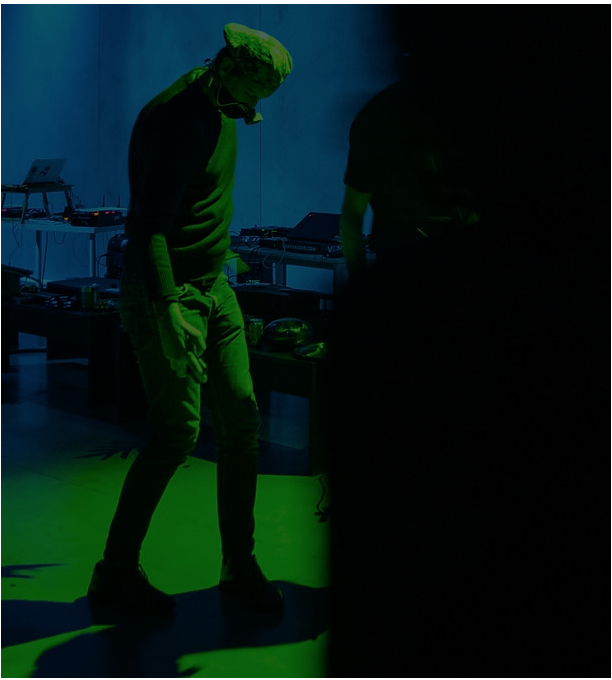
\includegraphics[width=0.75
\textwidth,keepaspectratio]{Chapters/Figures/adse_ess/CSL_MASK_MICK.png}
{\caption{Performer with Mask Wearable Sensor
}\label{fig:sensor_model}}
\end{figure}

\subsection{Introduction}
% \label{sec1}

The Coronavirus Disease 2019 (COVID-19) was affirmed as a pandemic by the World Health Organization (WHO) on 11th March 2020 \citep{cucinotta_who_2020} presenting numerous unforeseen novelties given that symptoms would range from severe to unrecognisable over an indeterminate timeline \citep{woelfel_clinical_2020}. As the effects of the pandemic intensified on a global scale, central governments enforced new regulations that compromise public space interactions against the preceding normality. While the specific constraints varied between countries and eased accordingly over time, a key component throughout was to prohibit physical contact almost entirely where viable and to avoid close proximity with others \citep{toquero_challenges_2020, department_of_health_and_social_care_coronavirus_2020}. Simultaneously, the sudden ubiquity of protective face coverings has introduced a plethora of unanticipated complications regarding verbal and non-verbal expressions that are habitually relied upon to interpret emotional states \citep{marta_i_2020,carbon_wearing_2020,grundmann_face_2020}.

In accordance with these measures, a vast majority of public events were jeopardised, particularly in the case of live performances and artistic installations. As pandemic regulations were gradually alleviated however, public activities were re-authorised on the grounds that all participants complied to mask-wearing and distancing orders \citep{safe_communities_covid-19_2020}. Moreover, efforts to minimise viral transmission brought new risks associated with wearable sensor technology, which is heavily reliant on physical contact around susceptible areas of the body, endorsing research and development in remote monitoring solutions \citep{seshadri_wearable_2020,jeong_continuous_2020}. We foresaw an experimental convergence of the spatial qualities of the onstage performers and the tensions on interpersonal conduct carried out in public. The notion of physical distance between bodies discloses a high dimension of non-verbal social cues \citep{kroczek_interpersonal_2020,vinciarelli_towards_2011,sundstrom_interpersonal_1976}. However, these inferences can deviate massively between individuals, and therefore, it’s unintuitive to commit to a one-size-fits-all model that is wholly representative of all sort of social contexts and cultural environments \citep{yu_investigation_2020,sorokowska_preferred_2017}.
% given the abundance of supporting evidence, first taking a global survey carried out by \citeauthor{sorokowska_preferred_2017} \citeyear{sorokowska_preferred_2017} for a comprehensive view, in addition to a selection of regional studies \citep{yu_investigation_2020,aliakbari_investigation_2011,shuter_proxemics_1976} which address attitudes towards social status, while \cite{dahl_hiding_2020} offer considerations for public space behaviour with regards to surveillance and policing.  

We propose an intervention to challenge the conventional dualisms between physical distancing and social connectedness, based on sound and movement. This begins by reconstructing our approach to both sensor-based monitoring and the delivery of live performance, looking beyond the introspective experience, and consider affective processes that occur externally from the body. We then present a wearable system for sound-movement interaction centralised around interpersonal distance and collective movement. Following a series of ideation sessions, over a two week period, the system was situated in a live performance setting from which we evaluate the performer's quality of movement in relation to the sound feedback. We describe some of the system’s key influences contextualised in the socio-emotional domain, inducing entrainment, spontaneity and awareness.

Our work continues to extend the rich design space for collective sound environments with movement sensing. We outline our perspectives on mediating social interactions with regards to the proposed coupling of distance sensing with sound actuation. Following this, we acknowledge the vital limitations of our initial framework and put forward research opportunities that may arise from extended exploration. Namely, the incentive of transitioning into open public environments where participation can occur pervasively. Additionally, we document the necessary measures taken with respect to the restrictions put into force by the COVID-19 pandemic; the impact of which remains prevalent up until the time of writing. Howbeit, our findings should be interpreted as universally relevant towards orchestrating spatially aware interventions even in non-pandemic circumstances. 
\section{Background}
\label{sec2:Background}

\subsubsection{Social Distancing and Public Presence}
\label{subsec:public_space}

It is evident that regular social engagement plays an important role in community wellbeing. Not only bonding with our close companions in organised situations, but inclusive of unanticipated interactions that emerge in public \citep{ang_your_2021,simoes_aelbrecht_rethinking_2010,sugiyama_associations_2008}. Progressive urban space planners have taken this into account, and been considerate of the spatial arrangements that help to encourage spontaneous encounters \citep{latham_social_2019,okkels_urban_2018,mehta_look_2009}. The first wave of the COVID-19 pandemic elevated some attention to this. The course of existing outside of our own home meant weighing out the chances of a life-threatening infection against the consequences of avoiding social connection, endangering one's health in other ways \citep{brooks_psychological_2020,rivera_effects_2020,zorzo_adult_2019,evans_social_2019}, that is, to even fathom an intuitive protocol under such agonising circumstances.

As emergency COVID-19 measures were becoming standardised globally, epidemiologists from the WHO firmly recommended a linguistic shift from \textit{social} to \textit{physical} distancing on the basis that modern technology is capable of keeping us connected in spite of the new regulations \citep{romania_interactional_2020}. We appreciate here that the anticipation of the first wave would in essence reject in-person contact in the way it was known; this narrative was therefore appointed to the normalisation of fully remote communication. But as society would phase in and out of non-confinement periods, conventional face-to-face interaction could take place again, persisting with the caution of physical distance, embracing \textit{Social Proximity} as a safe practice for social wellbeing \cite{long_covid-19_2021}. Irrespective of this major adaptation to safer re-socialisation, we argue that the development of in-person interventions have not matured to the same extent as remote interaction technologies, and that there still lies a vast domain in design for spatial sensitivities yet to be fulfilled.


\subsubsection{Proxemic Behaviour and Re-socialisation}
\label{subsec:Proxemic}

The attention towards interpersonal distance as a social cue coincides with the study of proxemics, examining the function of space during social interactions \citep{hall_hidden_1966, guerrero_proxemics_2015}. Proxemic theory has been given a lot of attention in a wide scope of behavioural studies \citep{mccall_mapping_2017} and thus spurring incentives from several ubiquitous computing projects \citep{perez_mobile_2020, marquardt_proxemic_2015}. A large proportion of these studies accept the proxemic zones set out by \cite{hall_hidden_1966}, by which interpersonal distances are generally categorised into the following boundaries: \textit{Intimate}, up to 1.5 feet; \textit{Personal}, 1.5 to 4 feet (1.2 m); \textit{Social}, 4 to 12 feet (3.6 m); and \textit{Public}, more than 12 feet (7.6 m). We believe however, that the rich contextual nature of interpersonal movement behaviour poses a challenge for conventional computational modelling, calling for expertise to break down and articulate expressive features of human motion and sensation \citep{fdili_alaoui_how_2015,schiphorst_self-evidence_2011}. With regards to proxemics, we cannot solely depend upon the measure of distances and angles to define the affective characteristics the occur during any given exchange.

Coping with the current risks of infection in everyday social contact, the \textit{new sociable space} implies a new urban etiquette that expands upon the standardised dimensions proposed by Hall's proxemic theory, preserving conversational affordances at double the distance \citep{mehta_new_2020}. In a general sense, spontaneous, informal encounters are recognised as an essential part of growing one's social circle, fostering a sense of belongingness within their community \citep{ye_ambivalence_2016}. However, the circumstances for which these are likely to occur are vulnerable to the spatial dynamics and physical distance between bodies \citep{van_den_berg_subjective_2017, fayard_photocopiers_2007}. These types of relationships fit into the social formation of indirect contact, which can take place seamlessly by way of intergroup behaviour, alleviating the pressures of face-to-face enactment \citep{white_beyond_2021} that are increasingly present in the midst of pandemic concerns \citep{durnova_intimacy_2021}. While of course, many will long to reconnect with their peers during moments of close physical bonding, these new sociable spaces provide an enlightening deconstruction of proxemic acceptability where strangers and non-strangers are both welcomed into everyday social encounters. The linguistic connotation towards 'distancing' assumes active separation from others, while it's function should instead be geared towards social affirmation, organised in a safe manner. We propose an interactional view on social distancing that's unconditional to definitive measurements, advancing upon the outlooks contained in the following study \citep{ballendat_proxemic_2010} that insists on expanding Hall's discrete interpretation of proxemic zones when applied to continuous mappings of movement. 

The orchestration presented in this case study is set out to capture the affective outcomes when proxemic behaviours are exaggerated during social exchange, where sensory intervention goes beyond being an assessment tool, but a modality for non-verbal expression.

\subsubsection{Sensor Technology and The Right to the City}
\label{subsec:shift}

% The right to the city & inclusion
Certain demographics are more sensitive, while others are far less cautious of invading the personal space of others \citep{peimani_where_2016,remland_interpersonal_1995}. Take for instance, the precautionary measures imposed onto women and men when approaching a crowded pedestrian area, where an imbalance that has been documented in several personal accounts (e.g. \cite{hewitt_i_2021}), in addition to extensive population surveys \citep{matsumoto_gender_2016,rosenbloom_crossing_2009}. In the perspective of present-day planning practices, the gendered landscape implies that equality is embedded into urban structures, namely access to safe open spaces and mobility behaviour, exemplified in the following case study of Umeå, Sweden \citep{sandberg_imagining_2016}. Complimentary to this outlook, the long-standing notion known as \textit{the right to the city} has been used in various contexts to express the destructive parallels between contemporary urbanisation and social inequality \citep{harvey_rebel_2012}. These concepts have recently been embraced by Interaction Design researchers, commentating on the industrialised approach that we are seeing with sensor technology that's being increasingly embedded into urban spaces, shifting the perspective from data-driven smart cities to \textit{social} or \textit{playful cities} \citep{castro_seixas_urban_2021,howell_life-affirming_2019}. Such case studies express a necessity for inclusive participation to establish grounds for progressive social integration, framed as the collective right to be in control of the surroundings through co-creation.

Urban pedestrian areas have long exemplified the effectiveness of street-installed technology to manage the mobility of crowds, however, the vital function is vulnerable to being overthrown in the case of high-intensity overcrowding \citep{gehl_public_2004,machleit_perceived_2000}, which has been associated with feelings of anxiety, frustration and claustrophobia \citep{kendrick_user_2010}. In respect to interpersonal distance, initiatives in response to pandemic conditions rely upon a level of altruistic responsibility, by which the public are inclined to follow a protective etiquette \citep{honey-roses_impact_2020}. When taking a look at the technologies that have become ubiquitous in response to the pandemic: Contact Tracing Applications, Skin Temperature Scanners, and contactless patient monitoring, for example \citep{mehrdad_perspective_2021,taylor_review_2020}, we note that the user is constrained to one interpretation of the data made available to them. When contrasted with alternative interventions that explore emotional bonding in urban environments, e.g. \citep{adhitya_london_2018,gatehouse_feral_2016}, we begin to question the limitations of the prior, and subsequently, practices that exist at the intersection of social affirmation and long-lasting public health. Building upon the insights presented by \cite{howell_life-affirming_2019}, calling for a progressive turn in public space sensing, we insist that the data-driven motives pushed onto current smart city development schemes are non-compliant with these sort of shared emotional experiences \citep{battarbee_pools_2002,lange_owning_2013,bueno_smart_2016}. Acting upon the current situation, we enquire into a sensory intervention that aids awareness to one's physical presence and self-affirmed boundaries, without the need to declare any action as right or wrong.

\subsubsection{Appropriation of Social Distance and Interpersonal Touch}
\label{subsec:safety}

The urgent nature of the pandemic demanded disruption to common interactional norms, namely in the concern of keeping distance and avoiding touch \citep{long_covid-19_2021,katila_interaction_2020}. But despite a reactionary appeal for spatially-aware behaviours, this call for action has been relevant for a while now. There exist several rationals for designing systems that are considerate of one's personal space, which in our view, have been neglected by relevant research areas. For many, the apprehension of close contact serves as an evaluation criterion for everyday safety, as conveyed by feminist enquiries into urban space \citep{farina_moving_2021,peimani_where_2016}. A preference for greater interpersonal distances is also evident for those suffering from anxiety disorders, commonly assumed as an avoidance of social interactions entirely \citep{givon-benjio_biased_2020}. Intersecting this view with the subjective quality of skin-to-skin contact, praised by a substantial volume of research for inciting profound therapeutic sensations \citep{crucianelli_developmental_2020}, presented as an appealing cure-all method to relieve anxiety, strengthen social bonds, and even elicit physical benefits \citep{field_touch_2010,peterson_parents_2007,dolin_reach_1993}. But this is not always the case if we take into account, for instance, those who experience hypersensitivity (or lack of) to introspective stimuli \citep{bischoff-grethe_neural_2018,sivik_alexithymia_1993}. The perceived benefits associated with affective touch are largely subject to the qualities of the pre-existing relationship of the dyad \citep{gulledge2007non}.

Drawing parallels with inclusive proxemic interventions and the new referential for safe re-socialisation \citep{long_covid-19_2021}, we want to understand the liberties that can emerge from contact-less mediation while protecting the right to physical presence. Therefore, to depart from the assumption that everybody is entirely comfortable with close contact, and understand that the degree of comfort largely depends upon who is approaching them and in what context \citep{matsumoto_gender_2016,suvilehto_topography_2015}. In Section \ref{sec5:discussion}, we discuss the importance of flexible boundaries when designing for interpersonal distance, conditional to the social context at hand and the proxemic sensitives of the individual.

\subsubsection{Non-verbal Contingencies and Face Coverings}
\label{subsev:face_coverings}

% As we commentate on the new social practices that are being introduced by pandemic regime, we should not undermine the inherent reliance on non-verbal expressions in virtue of restricted visibility of facial expressions or clarity of speech \citep{trujillo_speakers_2021}. 
% \citeauthor{hadley_synchrony_2021} \cite{hadley_synchrony_2021} point close attention to the use of physical gestures as a substitute for verbal exchange where background noises impair mutual comprehension of the voice. 
Proxemic interactions, given the alliance with mutual gaze, would assume the inclusion of facial expressions, where conventionally, more salient emotional attributes are depicted between the nose and the chin \citep{fischer_veiled_2012,blais_eyes_2012}. Knowing this, we should not undermine the inherent reliance on non-verbal expressions in virtue of restricted visibility of facial expressions or clarity of speech \citep{trujillo_speakers_2021}. This non-verbal exchange is highly relied upon in everyday life, but the regulated use of the face mask disregards this modality almost entirely \citep{carbon_wearing_2020}. This becomes even more crucial in the context of physical distancing regimes \citep{campagne_problem_2021}, where proxemic studies report a habitual reduction of eye contact when spaced more than twelve feet apart, i.e \textit{public distance}\citep{baldassare_cultural_1975}.

Our facial muscles can expose a great deal of how we are feeling \citep{qian_effects_2018,todorov_face_2017}, sometimes completely unknowingly to the extent that one may exert themselves into forcibly concealing these expressions while under pressure, coining the now popularised term "poker face" purposed to deceive opponents, thus framing the more generalisable action of "bluffing" \citep{billings_challenge_2002}. In comparison, how we move in space is normally a consequence to deliberate coordination during interaction \citep{poyatos_interactive_1980,jones_communication_2016}. \citeauthor{hadley_synchrony_2021} \citeyear{hadley_synchrony_2021} point close attention to the use of physical gestures as a substitute for verbal exchange where background noises impair mutual comprehension of the voice. A similar instinct can be assumed for many instances of everyday conversation cautioned by pandemic regulation \citep{campagne_problem_2021}, whereby the normalisation of face masks worn during conversation has been shown to degrade the acoustic quality of the voice as a result of suppressing higher frequencies ranges, commonly depended upon to recognise articulations of consonant sounds \citep{saunders_impacts_2021,rahne_influence_2021,nobrega_how_2020}. This poses a further disadvantage to those hard of hearing \citep{mckee_overcoming_2020} as well as non-native speakers, who have commented on their dependence on reading the face to better understand foreign dialogue \citep{inceoglu_language_2021,jabber_non-verbal_2020}. 
 
We propose that a mask-worn sensory device forms a deconstruction to habitual conversational norms, isolating communication channels aside from the face. In Section \ref{subsec:fabrication}, we outline our fabrication methods, taking the newly ubiquitous face mask, commonly condemned as a social hindrance and reshaping this as sensory material for non-verbal exchange.
 
\subsubsection{Measuring Interpersonal Movement}
\label{sec2_measuring}

Qualities of interpersonal movement are recognised by Rudolf Laban's Movement Analysis (LMA), a well-established notation framework used to depict expressive features of human movement, originating from the perspective of dance and physical therapy \citep{laban_mastery_1988}, and since adapted to all kinds of contexts (e.g routines of factory workers) \citep{davies_beyond_2006}. With ongoing advancements towards body-centred applications, Laban's theory on movement has firmly settled itself into Human-Computer Interaction research \citep{ziegelmaier_laban_2020}. This practice continues to be relevant in several state-of-the-art research fields, such as activity recognition \citep{ajili_robust_2017,truong_laban_2017}, gesture sonification \citep{fdili_alaoui_seeing_2017}, and movement modelling for virtual agents \citep{durupinar_perform_2017, ajili_robust_2017}. 

It's apparent here that the intersections of HCI and Laban Movement principles tend to focus on the kinematic or spacial-temporal qualities, which are modelled for individual accounts. Pluralist qualities, on the other hand, comprised of two or more persons moving together, are observed as the \textit{Relationship} category. The following article from \citep{roudposhti_parameterizing_2012} affirms a scarcity of literature in this domain, expressing the unexplored potential for social interactive systems. The authors propose a global feature space that combines Pentland's analysis model of social signals \citep{pentland_honest_2010} with LMA qualities, taking upon the following descriptors: \textit{Indicator}, \textit{Empathy}, \textit{Interest} and \textit{Emphasis}. We borrow two of these qualties in our evaluation, \textit{Inicator} to describe the exchange between influent and influecned members, presumed by the difference in energy between them, and \textit{Interest} respresenting one's engagment to the sitation or outside context, gauged by energetic movements. Similarly to Laban's Movement Analysis, each quality operates on a continuous scale between two polarites.

\subsubsection{Sound Interaction as Social Mediation}
\label{subsec:soundInteraction}

Throughout the extensive literature surrounding proxemic interfaces, we came across a surprising lack of studies related to sound, given this is already an established modality for movement interaction with ties to affective representation \citep{landry_interactive_2020}, supported by a base understanding that physical action and sound perception are mutually responsive \citep{krzyzaniak_six_2019}. As a tentative presumption, we can point to the inherent limitations of distance detection with typical camera-based tracking technologies \citep{wu_out_2017} as well as the obtrusiveness of on-body sensor devices \citep{hensel_defining_2006}. An affirming study that fits into this criteria \citep{rector_eyes-free_2017} installs a proxemic augmentation into a gallery space, supporting the role of proxemic audio interactions in a \textit{"post-screen world"} \citep{bryan-kinns_interaction_2017}. Our preliminary survey of sensor actuation couplings (see Section \ref{cha:Preliminary_Actions_sens_act}) demonstrates the usefulness of audio-based biofeedback as a way to foster physiological synchronisation and somatic awareness, noting that the human hearing system is highly sensitive and that sound is a convenient medium to share amongst many users. 

% We embrace sonic feedback as an appropriate mediation between the users that are directly interacting with the system, in company with external participants who engage as observers; from the perspective of an audience or otherwise \citep{francoise_designing_2017}

Within the context of music performance, the concept of a collaborative system is not a novel phenomenon, far from it in fact. Reports date back as far as 1978 \citep{bischoff_music_1978} originating from local network systems with progressions to real-time remote interaction using web-based servers \citep{barbosa_displaced_2003}. This supported the foundation for deeper research since the 2000s alongside the establishment and maturity of interactive music systems (IMSs), e.g. \citep{jorda_reactable_2007,freeman_auracle_2005}. In a recent review, \cite{aly_appropriating_2021} discuss the pervasive nature of sound interactions in the context of biosignal-driven IMSs when capturing data from many users simultaneously. In the context of live performance, \citeauthor{hege_spirit_2014} presents an artefact by which the members of the Princeton Laptop Orchestra showcase democratic expertise through intentional yet delicate control over the sound output, upheld throughout a prolonged structure of distinct phases. IRCAM researchers advocate towards a human-centred framework for gestural sound control in a group scenario \citep{schnell_collective_2015}, not only for performance, but also justified in clinical use-cases \citep{bevilacqua_exploring_2018}.

Moving away from the audience-performer dynamic, these shared experiences lend themselves well to the prospect of mediating human to human interactions in public. Case studies from \citep{roo_physio-stacks_2020,howell_life-affirming_2019,ashford_eeg_2019} recognise the potential of rich interpersonal interactions mediated through a shared interface, enabling a third-person perspective on the subject’s physiological activity. We would like to further investigate how human-human interactions can be augmented through embodied sensor data from multiple users, in this instance, representing an assembly of interpersonal distances through sound.

\subsection{Materials and Method}
\label{sec3:method}

\subsubsection{Composition of a Wearable Sensing Medium}
\label{sec3.1:tech_composition}

We decided to design a wearable sensing medium centred around the face mask. These were a mandatory possession for local citizens that had already become a cultural norm for one’s appearance in public \citep{cdc_covid-19_2021}. Our pursuit towards an on-body device was supported by \citeauthor{montanari_measuring_2018}'s \citeyear{montanari_measuring_2018} investigation into a novel proxemic sensor, welcoming a sacrifice in the high-level attributes that come with camera-based tracking in preference of environmental flexibility, quoting the affordance \textit{"to collect data even in areas that cannot be instrumented, like public spaces or during large events"}. In contrast to past studies on interpersonal movement which often make use of optical motion capture systems \citep{hale_are_2020,solberg_group_2019,hamilton_seeing_2018}, we consider the worthwhile benefits of a wearable solution that's more versatile in non-laboratory situations. \citep{hale_are_2020,solberg_group_2019,hamilton_seeing_2018}. In essence, this bypasses the challenges articulated by \cite{jurgens_designing_2020} directed towards using an unobtrusive markerless motion capture technology in an on-stage environment for contemporary dance performance. The authors highlight digital errors inflicted by particular lighting conditions, clothing contrast, as well as scenarios where performers were in close proximity to each other. For our study, we were incentivised to capture the point of view of the user, aligning the sensing trajectory with the user's gaze during interaction, as detailed in the following sections.

\subsubsection{Overview of Components}

% We have interfaced low-cost HC-SR04 ultrasonic distance sensors with a WiFi-enabled microcontroller\footnote{BITalino R-IoT Datasheet:  \url{https://bitalino.com/storage/uploads/media/datasheet-r-iot---v12.pdf}}, enabling the acquisition and streaming of proxemic data from multiple participants. Fundamentally, the sensor measures the distance from the first physical interference at a given direction by transmitting and receiving ultrasonic frequencies outside of the human hearing range \citep{pal_distance_2015}. The range and accuracy benchmarks for the ultrasonic sensors are partially dependent on environmental variables such as ambient temperature and humidity. When working in typical indoor conditions, the ultrasonic sensors are expected to ensure a stable accuracy up until 13 feet. We incorporated temperature data into the distance acquisition function, this improved the reliability and consistency of the readings when transitioning between distinct environmental conditions. For example, a computer lab, open exhibition space, performance theatre holding maximum occupancy, or even installed in an open outdoor area. Technical Specifications have been included in the (Supplementary Material))

We have interfaced low-cost HC-SR04 ultrasonic distance sensors with the BITalino R-IoT microcontroller using a modified firmware (included in the (Supplementary Material); this allows the acquisition of proxemic data from multiple participants at 10 samples per second. When initiated, each module streams data wirelessly over a designated local Wi-Fi network to a host computer, which is then responsible for signal processing and sonification. This sensing technology is highly prevalent in robotics and IoT educational fields, typically used as part of introductory curricula \citep{hernandez-barrera_teaching_2014,garcia-ruiz_integrating_2018} while sustaining relevance in the state of the art (e.g., \cite{eguchi_proto-chair_2020,xu_analyzing_2018}). Fundamentally, the sensor measures the distance from the first physical interference at a given direction by transmitting and receiving ultrasonic frequencies outside of the human hearing range \citep{pal_distance_2015}. The range and accuracy benchmarks for the ultrasonic sensors are partially dependent on environmental variables such as ambient temperature and humidity. When working in typical indoor conditions, the ultrasonic sensors are expected to ensure a stable accuracy up until 13 feet.

With respect to providing a wearable form factor, minimising the size and weight of the components, we implemented a discrete voltage divider onto the sensor’s Ground and Echo pins to comply with the power specifications commonly found in smaller microcontrollers, usually rated at 3.3 Volts. With this configuration, there was a minor but notable drop in accuracy compared to our tests using 5-Volt compatible microcontrollers. However, this was mostly resolved with signal processing to the extent that the effects would not hinder the overall sound-movement experience. Following technical directions from Kielas-Jensen \citep{magicbycalvin_improve_nodate}, we were able to incorporate data from the R-IoTs embedded temperature sensor into the distance acquisition function, this improved the reliability and consistency of the readings when transitioning between distinct environmental conditions. For example, a computer lab, open exhibition space, performance theatre holding maximum occupancy, or even installed in an open outdoor area.  

\subsubsection{Material Design and Fabrication}
\label{subsec:fabrication}

In order to publicly distribute the sensory masks in a safe manner, respecting the government guidelines, we assigned the following design principles: (1) The sensory components are modular and detachable, allowing the interchange of mask fabric and application of a suitable sanitation solution; (2) these components must remain at a fixed position and be robust in situations of rapid movement; and (3) the mask should feel sufficiently comfortable for users to wear for prolonged periods of time. Additionally, for the system to accommodate mass participation, we favoured (4) a scalable solution that was low-cost per unit and easily reproducible. For each wearable, we modelled two separate housing elements for the respective components, i.e the microcontroller and the proximity sensor. The 3D models are included as part of the (Supplementary Material). 

For the sensing mechanism, the ultrasonic sensor casing was merged with an arched nose clip and secured onto the mask fabric. The microcontroller and battery were encased in a custom mask strap that would be tied around the back of the head. The components are connected via a flexible cable, splitting into four wires each connecting to the corresponding inputs of the sensor and microcontroller, transmitting analogue signals back-and-forth to retrieve proximity data, represented as trigger and echo in Figure \ref{fig:sensor_model}. These are assembled by positioning the sensor component above the nasal dorsal, resting front-most of the face, in-line with the gaze with minimal obstruction. To overcome the precariousness of the sensors dropping down from the nose during movement, we increased the tension of the elastic ear straps and fastened a flexible rod between the mask fabric and sensor attachment. While this modification improved the structural reliability, our capacity to freely substitute sensory modules, along with spontaneous user alterations was now limited.

\begin{figure}[!h]
\captionsetup{width=1.0\textwidth}
\centering
\includegraphics[width=1.0
\textwidth,keepaspectratio]{Chapters/Figures/adse_ess/figure1_landscape_components_optimized.png}
{\caption{Proximity sensor enclosure fitted onto the face mask with trigger (output) and echo (receiver) signals.
}\label{fig:sensor_model}}
\vspace*{-20pt}
\end{figure}

\subsubsection{Data Processing and Sound Mapping Strategies}
\label{sec:mapping}

The orchestration by itself does not require participants to conform to a fixed minimum distance that is deemed compatible a particular behavioural model. We lend our trust to the users to coordinate themselves in a safe manner without explicit orders, the same way as is expected in their daily life. The sound interaction is purposed to strengthen each subject's awareness of the other's presence, unbounded from discrete categorisation. In addition to this, the experience should not call for virtuosity or a specialist training process. The system assumes engagement from the moment the user is being sensed and become progressively accustomed to the sound-movement affordances. This aligns with the presumption that the participants are non-acquainted with each other prior to the session, expected to work together to develop their understanding of the system, and stay vigilant to each other's actions.

During these first trials, we used granular synthesis \footnote{{Grain Scanner
by Amazing Noises: \url{https://www.ableton.com/en/packs/grreciprocateain-scanner-amazing-noises/}}} to interpolate between 4 field recordings as base sound textures. Inspired by Laban's qualities of space and relationship, we proposed a transition between "open" to "closed" sound textures as the average distance reaches the minimum sensing boundaries of 4 feet, before succeeding social distance. This process starts with a lot of fluctuations in timbre and then closes in on a limited range of frequencies that form into a staccato rhythmic feel. 
% Working with individual streams of sensor data for mapping, a smoothing filter was implemented for all devices to reduce digital artefacts and provoke slow, exaggerated movements, aimed to highlight the positional qualities in the performance space over time. After participants familiarised themselves with the interaction framework and initiated experimentation with more structured movement patterns, we would gradually reduce the smoothing coefficient by 50 per cent, increasing the sensitivity of the movement-sound relationship.

\begin{figure}[!h]
\captionsetup{width=1.0\textwidth}
\centering
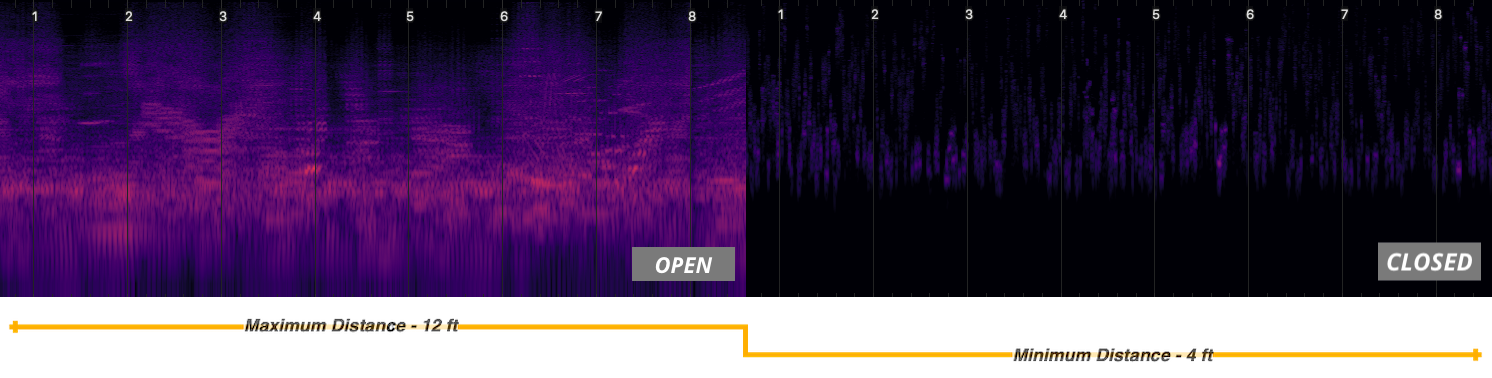
\includegraphics[width=0.8\textwidth,keepaspectratio]{Chapters/Figures/adse_ess/open_closed_examples_annotated_landscape_line.png}
{\caption{Spectrogram samples of "open" and "closed" sound textures}\label{fig:sound_examples}}
\end{figure}

\subsubsection{Performance Structure}
\label{sec:structure}

% We came to the realisation during the early stages of experimentation that simply giving a new group of users the wearable devices and initialising the sound output was not a sufficient means for physical engagement. 
Our prior expectations were that participants would be given the wearable and instinctively begin walking towards one-another in attempts to provoke the sound-movement mapping, where adversely, the system's initial deployment exposed a significant level of confusion from new users. Aside from the technical ideation, we speculated upon ways of stimulating movement whilst sustaining an appropriate degree of improvisational freedom. Reiterating that the participants were not highly experienced in dance or theatre disciplines, and we were not interested in forcing a strict movement sequence, but rather providing geometrically informed cues set out to prompt dyadic movement patterns. We devised three scenes that each focus on distinct affordances of proxemic mediation, as illustrated in Figure \ref{fig1:structure} and presented in the following order:

\begin{itemize}[align = left]
    \item[(i)] Geometric boundaries and interceptions 
    \item[(ii)] Interacting with the non-human
    \item[(iii)] Participation from external users
\end{itemize}

\subsubsection{Performers and Objects}
\label{sec:structure_2}

These geometric arrangements are predominantly inspired by William Forsythe's architectural approach to choreographic environments \citep{forsythe_dance_1999}, a radical staple in contemporary dance culture, bridging deeply into other artistic mediums \citep{clark_geometry_2014}. 

 The following passage redirects the proxemic attention from the neighbouring bodies, onto the surroundings (Figure \ref{fig1:structure} (ii)), supported by \citeauthor{bryan-kinns_mutual_2013}'s \citeyear{bryan-kinns_mutual_2013} recommendations for mutual engagement with shared representations. In the extended proxemic criteria presented by \cite{ballendat_proxemic_2010}, the relationship to other objects, both digital and nondigital is embraced. Adopting theories of gaze-based interaction into the format of proxemic awareness, authors claim to enrich the user's attention to the space by attending to implicit responses from the user's surroundings.
 
 Autonomous flying drones have been incorporated into stage performance \citep{eriksson_dancing_2019} and movement-centred practices \citep{la_delfa_drone_2020} proceeding efforts to enhance kinesthetic awareness through precise intercorporeal engagement \citep{tezza_state---art_2019}. During scene i, the drone represents more generally an unpredictable external influence, comparable to the external nuances that occur in public space settings.

 \citeauthor{ballendat_proxemic_2010}'s \citeyear{ballendat_proxemic_2010} evaluation of screen-based proxemic interactions considers the attention directed to other people, allowing for conventional social exchange to coexist alongside with the technological artefact itself, accepting natural influences that would arise in coherence with an everyday social situation.

\paragraph{Scene i, Geometric Boundaries and Interceptions}

To begin, the performers position themselves around the boundaries of the performance area, facing the centre (Figure \ref{fig1:structure} (i)). The first sounds are activated as users cross to the opposite side, alternating back and forth until coinciding with the linear path of one another, after which an anticipated diversion is required. One participant offers the following interpretation: \textit{"The soundscape intensifies as the collective tightens in space. Before collision, we have to figure out our next steps, to dodge, retrace or simply pause for a moment"}. Our improvisational framework here is designed to inspire proxemic exchange, while the primary responsibility of avoiding near-contact is handed over the to the performers.

\paragraph{Scene ii. Interacting with the non-human}

A drone technician is assigned the role of navigating the stage, weaving between the masked performers. When advancing towards the bodies on stage, specifically targeting the sensory components, the drone serves as an external trigger as it reaches close enough to the face. As a result, this synthetic artefact would provoke instantaneous reflex responses from the performers that would consequentially, instigate dynamic changes in the soundscape.

\paragraph{Scene iii, Participation from external users}

Finally, in Scene (iii), we invite external users that are not individually equipped with any wearable sensors but are authorised to manipulate the behaviour of the mask-wearing user group. The two collectives both march between the right and left extremities of the stage, constantly maintaining a mutual gaze and a forward distance of approximately 6-10 feet from the closest person opposite (Figure \ref{fig1:structure} (iii)).
% Similarly, with the inclusion of the surrounding objects as interaction modality, the authors willingly accept the external influences that would come naturally as part of an everyday social situation.

\begin{figure}[!h]
\centering
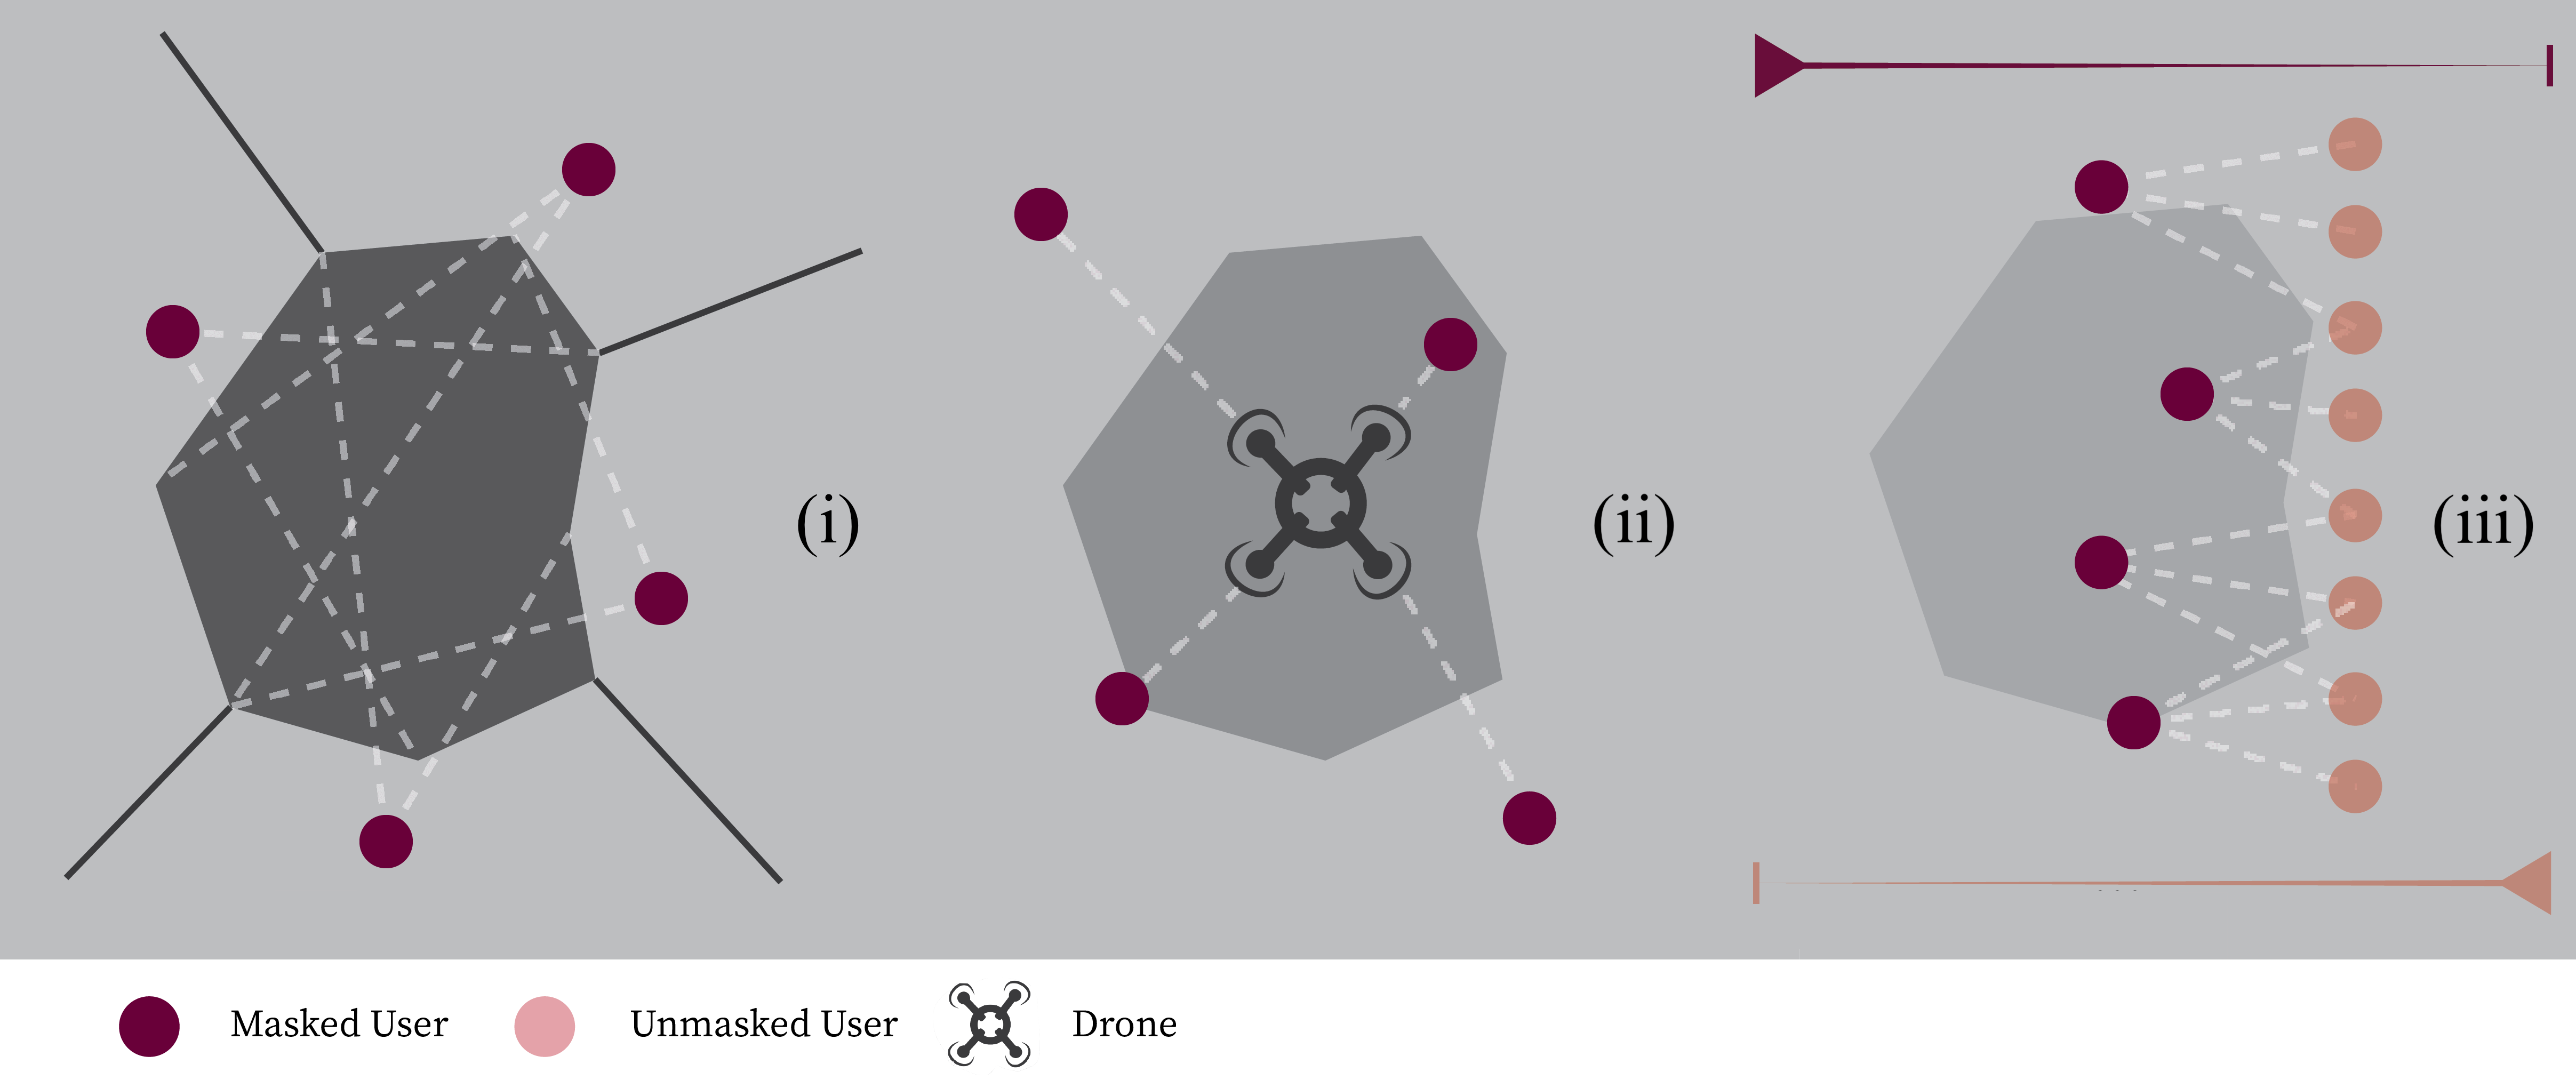
\includegraphics[width=0.9\textwidth,keepaspectratio]{Chapters/Figures/adse_ess/scenes_w_keycode.png}
{\caption{Visual representations for each scene}\label{fig1:structure}}
\end{figure}

\subsection{Study Outline}

Our study derives from the experimental framework of Performance-Led Research in the Wild \citep{benford_performance-led_2013}. This compromise relieves some of the social confines imposed in a lab setting while bypassing the highly unpredictable nature that comes with arbitrary participation \citep{heron_par_2017}. In this current research action, we setup an open call, 12 local artists were chosen to take part in a 2-week residency that would conclude with a public performance. This was structured to build upon compositional practices that were stimulated from a series of performance and improvisation workshops that took place 3 weeks prior. From the residency group, 4 participants were selected to use the wearable during the final performance, presenting the three scenes described above, which lasted just over 8 minutes in total. We recorded video and sensor data throughout each scene in order to evaluate the qualities of interaction. From this sub-group, 3 identified as male and 1 female with ages between 24 and 51 years old. All 4 held long term experience as highly-skilled musicians, performing internationally and retaining regular musical practice. An additional 4 participants, 50:50 split male and female, trialled primitive iterations of the system during the prior rehearsal stages, from which we produced field notes and recorded user feedback. Aside from a handful of local encounters, the user group were considered strangers amongst one another, not closely bonded and only acquainted during the residency. 

In the scope of COVID-19 distancing measures, the user group were respected as a support bubble throughout the research period, assuring that in-person interactions were permitted on the same conditions as those they share a home with \citep{trotter_ways_2021}. With that said, at no point would the sessions explicitly require a disruption to the standardised safety regimes, particularly those concerning close contact and sanitation of shared materials to minimise viral transmission.

% \subsection{Data Collection Sources}
% \label{sec:data_collection}

\section{Preliminary Results}
\label{sec:results}

Here, we summarise the perspectives from the individual participants and indicate moments where the first-person accounts are complemented by the acceleration data. We apply statistical analysis onto the collective sensor pool to discern group-level features, later used to substantiate relevant design guidelines for proxemic intervention strategies. We acknowledge the analytic restraints when subjected to a single recording from an individual user group, that by no means, should be taken as a comprehensive survey of the proxemic orchestration. This provisional study is purposed to demonstrate novel adaptations for proxemic interaction and prescribe design insights for future work.

%  Given the multiple directions of novelty, this provisional study is purposed to contribute to our discussion and prescribe design insights for future work.

% How did you get user accounts - after each session
\subsubsection{Data Collection}
\label{sec:data_collection}

% \subsubsection{First-person Accounts}
Throughout a 2 week prototyping period, we recorded participant observations and first-person experiences. This comprised of 8 day-long rehearsal sessions that each allowed one hour focused on exploring the wearable followed by a brief interview; these took place alongside a course of improvisation exercises fitted towards musical performance. After the study, we extract comments from a series of recordings and field notes.

We recorded video and audio of the final performance and rehearsals using single point microphone and camera. The video clips were colour graded to obtain a clearer view, especially when there was a lack of ambient light being projected onto the stage. When probing deeper into a handful of significant events depicted by our written assessment, we extract still frames from the recordings and overlay these with graphical annotations to commentate on the positional qualities present. Audio was processed through Sonic Visualiser\footnote{Sonic Visualiser: \url{https://www.sonicvisualiser.org/doc/reference/4.4/en/}} for feature extraction. The sensory masks were embedded with an accelerometer sensing component located at the back of the head, recording three axis of directional acceleration from each user. The triaxial sensor data is unified by computing the Signal Vector Magnitude (SVM), representative of the combined acceleration coordinates x, y and z, as validated by \citeauthor{ward_sensing_2018}'s \citeyear{ward_sensing_2018} proposed method for monitoring synchronous motor behaviour within a group of live performers. 

When probing deeper into a handful of significant events depicted by our written assessment, we extract still frames from the recordings and overlay these with graphical annotations used to commentate on the positional qualities present. In Figure \ref{fig:sensor_data}, we present the median average magnitude acceleration measured from the four user to represent the collective movement, indicated by a series of peaks throughout the three scenes. The median acceleration timeline (top) serves as a guide to navigate the general progression of movement qualities presented throughout the performance, while separating the data stream for each individual user (middle), and assessing the alignment of the peaks provides a numerical evaluation into interpersonal responsiveness, or absence of. Finally, the peak acceleration points are clustered according to a series of successive bursts, detected algorithmically (bottom). The clusters help us to convey the collective movement dynamics and relationship qualities that are observed throughout each scene, partly revealed in the average duration and amplitude of the clusters. We formulate the following clustering features: \textit{peak density}, the total number of peaks detected relative to the duration of the cluster, and \textit{user effort dissimilarity}, based on an equal alteration of active users.

\begin{adjustwidth}{-9cm}{}
\begin{figure}[!h]
\centering
\includegraphics[width=1.0\textwidth,keepaspectratio]{Chapters/Figures/adse_ess/figure3_avg_median_peaks_clusters2_labeled.png}
\caption{Acceleration data recorded from scenes \textit{i}-\textit{iii}: the top row displays group median averages (1), with individual user data shown below (2). The final row aligns the peak cluster periods detected along the X axis (3).
a high-resolution version of the image is available in the (Supplementary Material))}\label{fig:sensor_data}
\vspace*{-20pt}
\end{figure}
\end{adjustwidth}

\subsubsection{Interpersonal Synchrony}

We trust synchronous motor activity to be a reliable indicator of prosocial affiliation \citep{hadley_synchrony_2021}, particularly when contextualised with sound, be it disruptive or complimentary \citep{solberg_group_2019}. During Scene iii, we observed participants engaging more confidently before and after the sound mapping is disrupted by the unmasked participants. In these moments, the mask-wearing group march in parallel alignment, maintaining a consistent pace with each other. Additionally, we note the persistent use of eye contact towards the unmasked group, voiding obstruction until reaching the end of the stage. As the procedural soundscape is overridden by the choral chants voiced from the unmasked performers, we see the groups disperse in the opposite direction, subverting the momentum and common alignment. This interplay repeats itself 4 times, where the two sub-groups voluntarily handover the leading role of the march, alternating every 6-10 seconds.

\begin{figure}[!h]
\centering
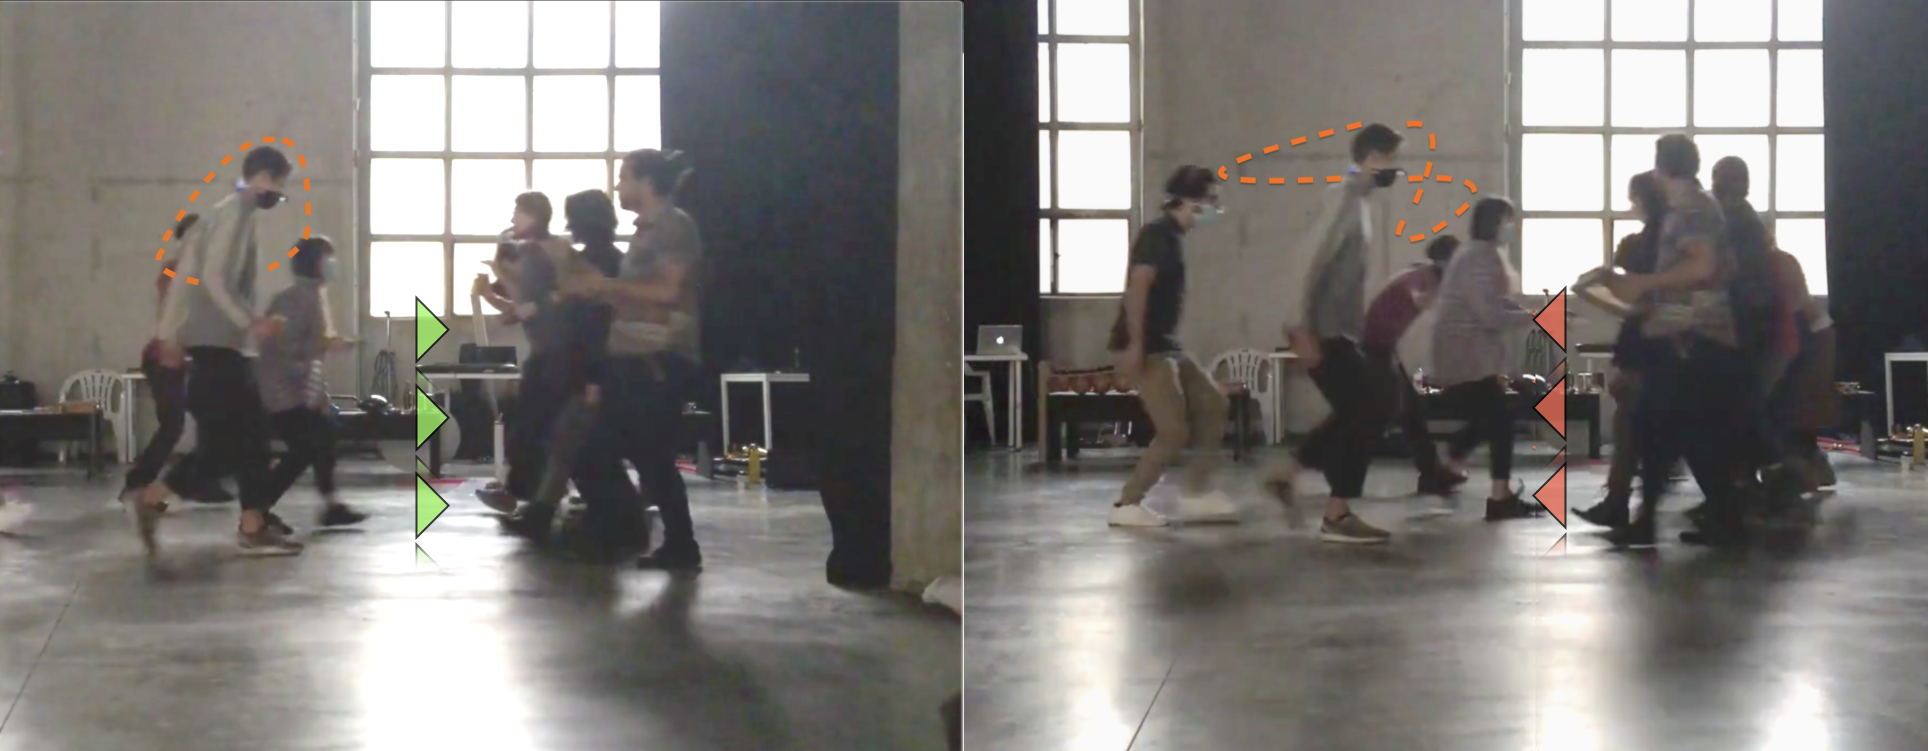
\includegraphics[width=0.9\textwidth,keepaspectratio]{Chapters/Figures/adse_ess/scene_iii-merged-2.png}
{
\caption{Annotations from Scene \textit{iii} rehearsal video. Four masked performers walk towards and away from a group of those without wearable sensors whilst maintaining a forward distance. The arrows show the walking direction with a dashed line to trace the dispersion of mask wearing group.
}
\label{fig:scene_iii_annotation}
}
\end{figure}
% \newpage

We compare the synchronous activity of each scene based on the separation of the clustered peaks. From this measure, we determine that the most consistent levels of synchronous movement take place during scene iii, with far fewer occurrences during Scene ii. Both scenes have a similar number of peaks per cluster (Table \ref{table:cluster_table}), with a greater density of peaks in scene iii; this is shown shown by the constrained duration of the clusters formulated in more consistent intervals. This perception is reassured by the increased amplitude of acceleration values throughout, perceived as an intentional syncopation of movements that are highly responsive to one another, agreeable to the feedback given by one of the users.

\begin{center}
\begin{tabular}{ p{13cm}}
\textit{we had only a short moment to be respond, similar to a call-and-response situation you sometimes see in concerts. The motivation was no longer about controlling the timbre (of the sound), but just to assert dramatic impulses before the others take the lead.}
\end{tabular}
\end{center}
 
Our observations and data taken from this final arrangement indicate vastly different group behaviours from before. We would suggest that the major influence lies behind the "call-and-response" routines as the opposing bodies assert themselves into the space, inducing a series of structured interruptions that we probe deeper into in the Discussion, \ref{subsec:sensibility}. We won't neglect here that these behaviours were inherently dramatised under theatrical persuasion, but nonetheless, insist that the core reactions are authentic to the invasive confrontation as the opposing bodies assert themselves into the space.

\begin{table}[!h]
\begin{adjustwidth}{0cm}{}
\centering
\resizebox{1.0\textwidth}{!}{%
\begin{subtable}[c]{1\textwidth}
\begin{tabular}{*{4}{l}}
\hline
\\[-1em]
Scene &
  \begin{tabular}[c]{@{}l@{}}Mean \\Peak\\ Interval (s)\end{tabular} &
  \begin{tabular}[c]{@{}l@{}}SD \\Peak\\ Interval (s)\end{tabular} &
  \begin{tabular}[c]{@{}l@{}}Median\\ Peak \\Amplitude (g)\end{tabular} \\
%   \begin{tabular}[c]{@{}l@{}}User Effort\\ Dissimilarity \\(\%)\end{tabular} &
%   \begin{tabular}[c]{@{}l@{}}Alternating\\ User Peaks\\ (\%)\end{tabular} &
%   \begin{tabular}[c]{@{}l@{}}Mean Cluster\\  Concentration\\(Peaks/Cluster)\end{tabular} &
%   \begin{tabular}[c]{@{}l@{}}Mean \\Cluster\\  
%   Duration (s)\end{tabular} \\
\\[-1em]
\hline
\\[-1em] 
\\[-1em] 
\textit{i} & \textbf{\databar[202.017391]{183.7}} & \textbf{\databar[164.887924]{149.9}} & \databar[0.390556]{0.31} \\ 
\\[-1em] 
\textit{ii} & \databar[202.017391]{182.1} & \databar[164.887924]{141.4} & \databar[0.390556]{0.29} \\ 
\\[-1em] 
\textit{iii} & \databar[202.017391]{155.8} & \databar[164.887924]{138.2} & \textbf{\databar[0.390556]{0.36}}\\ 
 \\[-1em] 
 
\hline
\end{tabular}
\begin{tabular}{*{5}{l}}

\\[-1em]
 &
%   \begin{tabular}[c]{@{}l@{}}Mean \\Peak\\ Interval (s)\end{tabular} &
%   \begin{tabular}[c]{@{}l@{}}SD \\Peak\\ Interval (s)\end{tabular} &
%   \begin{tabular}[c]{@{}l@{}}Median\\ Peak \\Value (g)\end{tabular} &
  \begin{tabular}[c]{@{}l@{}}User Effort\\ Dissimilarity \\(\%)\end{tabular} &
  \begin{tabular}[c]{@{}l@{}}Alternating\\ User Peaks\\ (\%)\end{tabular} &
  \begin{tabular}[c]{@{}l@{}}Mean Cluster\\  Concentration\\(Peaks/Cluster)\end{tabular} &
  \begin{tabular}[c]{@{}l@{}}Mean \\Cluster\\  
  Duration (s)\end{tabular} \\
\\[-1em]
\hline
\\[-1em] 
\\[-1em] 
\textit{i} & \databar[49.148936]{25.5} & \databar[106.206896]{90.2} & \textbf{\databar[4.900005]{4.5}} & \databar[10.957749]{8.9} \\ 
\\[-1em] 
\textit{ii} & \textbf{\databar[49.148936]{44.7}} & \databar[106.206896]{78.7} & \databar[4.900005]{3.8} & \textbf{\databar[10.957749]{10.0}} \\ 
\\[-1em] 
\textit{iii} & \databar[49.148936]{17.2} & \textbf{\databar[106.206896]{96.6}} & \databar[4.900005]{4.1} & \databar[10.957749]{5.6} \\ 
 \\[-1em] 
\hline

\end{tabular}
\end{subtable}
}
\end{adjustwidth}
% \vspace{5pt}

% \begin{table}[]
% \begin{adjustwidth}{-6cm}{}
% \centering
% \resizebox{0.65\textwidth}{!}{%
% \begin{subtable}[c]{1\textwidth}
% \begin{tabular}{*{8}{l}}
% \hline
% \\[-1em]
% Scene &
%   \begin{tabular}[c]{@{}l@{}}Mean \\Peak\\ Interval (s)\end{tabular} &
%   \begin{tabular}[c]{@{}l@{}}SD \\Peak\\ Interval (s)\end{tabular} &
%   \begin{tabular}[c]{@{}l@{}}Median\\ Peak \\Value (g)\end{tabular} &
%   \begin{tabular}[c]{@{}l@{}}User Effort\\ Dissimilarity \\(\%)\end{tabular} &
%   \begin{tabular}[c]{@{}l@{}}Alternating\\ User Peaks\\ (\%)\end{tabular} &
%   \begin{tabular}[c]{@{}l@{}}Mean Cluster\\  Concentration\\(Peaks/Cluster)\end{tabular} &
%   \begin{tabular}[c]{@{}l@{}}Mean \\Cluster\\  
%   Duration (s)\end{tabular} \\
% \\[-1em]
% \hline
% \\[-1em] 
% \\[-1em] 
% \textit{i} & \textbf{\databar[202.017391]{183.7}} & \textbf{\databar[164.887924]{149.9}} & \databar[0.390556]{0.31} & \databar[49.148936]{25.5} & \databar[106.206896]{90.2} & \textbf{\databar[4.900005]{4.5}} & \databar[10.957749]{8.9} \\ 
% \\[-1em] 
% \textit{ii} & \databar[202.017391]{182.1} & \databar[164.887924]{141.4} & \databar[0.390556]{0.29} & \textbf{\databar[49.148936]{44.7}} & \databar[106.206896]{78.7} & \databar[4.900005]{3.8} & \textbf{\databar[10.957749]{10.0}} \\ 
% \\[-1em] 
% \textit{iii} & \databar[202.017391]{155.8} & \databar[164.887924]{138.2} & \textbf{\databar[0.390556]{0.36}} & \databar[49.148936]{17.2} & \textbf{\databar[106.206896]{96.6}} & \databar[4.900005]{4.1} & \databar[10.957749]{5.6} \\ 
%  \\[-1em] 
% \hline

% \end{tabular}
% \end{subtable}
% }
% \end{adjustwidth}
% \end{table}
\caption{Peak and cluster statistics from each scene, calculated from the individual user acceleration data that corresponds to rows (2) and (3) in Figure \ref{fig:sensor_data}}
\label{table:cluster_table}
\end{table}
% \vspace*{30pt}

\subsubsection{Spontaneous and Sustained Engagement}

Given the premise that regular social engagement is an effective precursor to community wellbeing, generating and sustaining interactions are both considered to play a key role in urban design practices. We question how sensor-based mediation can be used to not only provoke, but actually extend the longevity and quality of an new encounter, described as, "what makes the experience comfortable, interesting, and meaningful" \citep{mehta_look_2009}. In this case study, we gauge spontaneous engagement from the rotation of users asserting themselves as leading influence (i.e. a new person exerting an acceleration peak), and how peaks are partitioned between individual users. Sustained interactions are more nuanced, recognised as lingering behaviours that take place amidst the succession of new movements, for which we draw upon the user's continuity of control with the sound output.

When examining the acceleration patterns shown in the two scenes ii and iii presented prior, we enquire into the user's relationship with the surrounding artefacts, and the way these momentarily interfere the continuity of the sound output, separating these external influences by their level of predictability. In Figure \ref{fig:interuptions-spectogram}, we recognise a major disparity in the arrangement of the non-structured interruptions incited by the flying drone compared to those anticipated by the unmasked group (i.e. structured interruptions). The unpredictable manoeuvres imposed by the flying drone disrupts the course of sustained dyadic gestures, from which we dissect the rapid, unplanned interchange of users controlling the sound output. Referring back to Figure \ref{fig:sensor_data}, this parallels with sporadic changes in peak intervals, with individual exertions coming at arbitrary intervals. Scene iii on the other hand, the course of sonic deviations better emphasise a uniform sequence of interruptions. This repeatable turn in controllability infers an attentive reciprocation with the other users, showing an advancement from sporadic reflex actions to meaningful group gestures, also granted by steadier peak intervals and the overall progression of synchronous movement that's detailed in the subsection above. One participant describes an impulsive reaction while being approached by the flying drone, suggesting its non-human form carries a provocation for spontaneous engagement:

\begin{center}
\begin{tabular}{ p{13cm}}
\textit{the drone would keep coming closer, like I was being chosen out of the crowd, so I would start following. I was comfortable with running towards the wall or even a flying object, but into somebody else, it's not the same. Even if we do not get so close, I feel like I am threatening someone or just being a nuisance.}
\end{tabular}
\end{center}

This correspondence is not so apparent in the acceleration data, where we actually notice a drop in energy regarding the lower mean cluster density and substantial user effort dissimilarity, supposing an imbalance of individuals dominating the space. Though, we may testify that the shared positional influence of the drone on stage engaged all users to the shared space, even when at a standstill.

\begin{figure}[!ht]
\centering
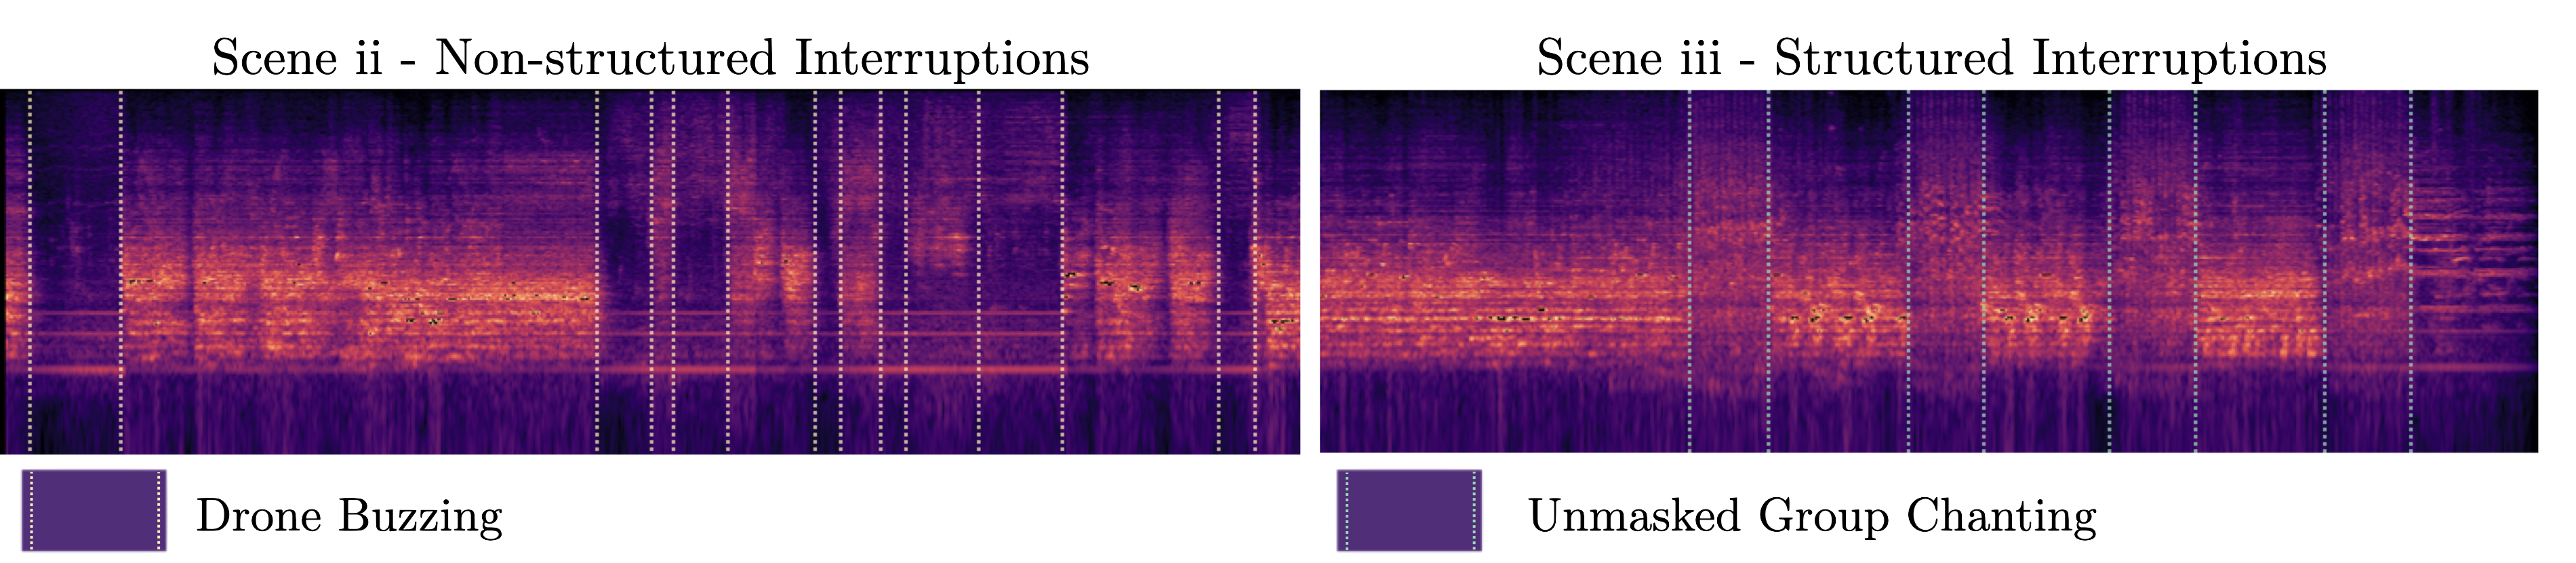
\includegraphics[width=\textwidth,keepaspectratio]{Chapters/Figures/adse_ess/interuptions-spectogram-markings-fig.png}
{\caption{Spectrogram recording from two scenes, \textit{ii} and \textit{iii}, marked with interruptions of the granular soundscape}
\label{fig:interuptions-spectogram}}
\end{figure} 

\subsubsection{Technical Venerability against Proxemic Awareness}
\label{subsec:accuracy}

In hindsight, the placement of the sensors of the face, constantly shifting their projected angles meant that misreadings were highly probable. When tested in lab conditions, these proximity sensors are expected to perform reliably at differing trajectories \citep{abreu_low-cost_2021}, but when we inspect the sound recording and video footage, we observed many cases of unexpected readings during the performances in contrast to the testing phase. Participants would move closer together and with no perceivable feedback. Moreover, the detectability of the ultrasonic reflections was highly dependant on the material of the occlusion. Figure \ref{fig:material_comparison} provides a set of sample signals recorded when approaching the sensor using three different surfaces. The ceramic tile provided the greatest detection range, while the clothing material resulted in more noise and venerability to drop-outs. Though our signal filtering methods helped remove extreme anomalies, there would still be a great deal of inaccurate measurements being fed into the system. For these reasons and more, this particular sensor technology has been discouraged for measuring interpersonal distance in a review of wearable devices for proxemic interaction, which exposes multiple scenarios by which ultrasonic sensing was proven to be partly inadequate \citep{montanari_measuring_2018}. 

\citeauthor{fdili_alaoui_making_2019} \citeyear{fdili_alaoui_making_2019} writes about the perceived messiness that inevitably comes with adopting personal tracking devices into performance-based practice (noise, sensor placement, classification failure). However, instead of seeing these as issues that need to be resolved, actually encourages artists to embrace the technical nuances, turning technology resistance into creative material. It's important appreciate that in non-lab conditions, imperfections will constantly prevail and therefore, we should welcome and validate the experiences that come with each iteration. In spite of such cases where the sound-movement relationship was not sensible to the performer or even the audience, as revealed repeatedly during the user studies, we contend that there remained a genuine influence from the physical artefact alone. Throughout the study, users demonstrated a strong awareness to their surroundings to control the sounds, recognising technical faults and overcoming them through persistent trial and error.

\begin{figure}[!ht]
\centering
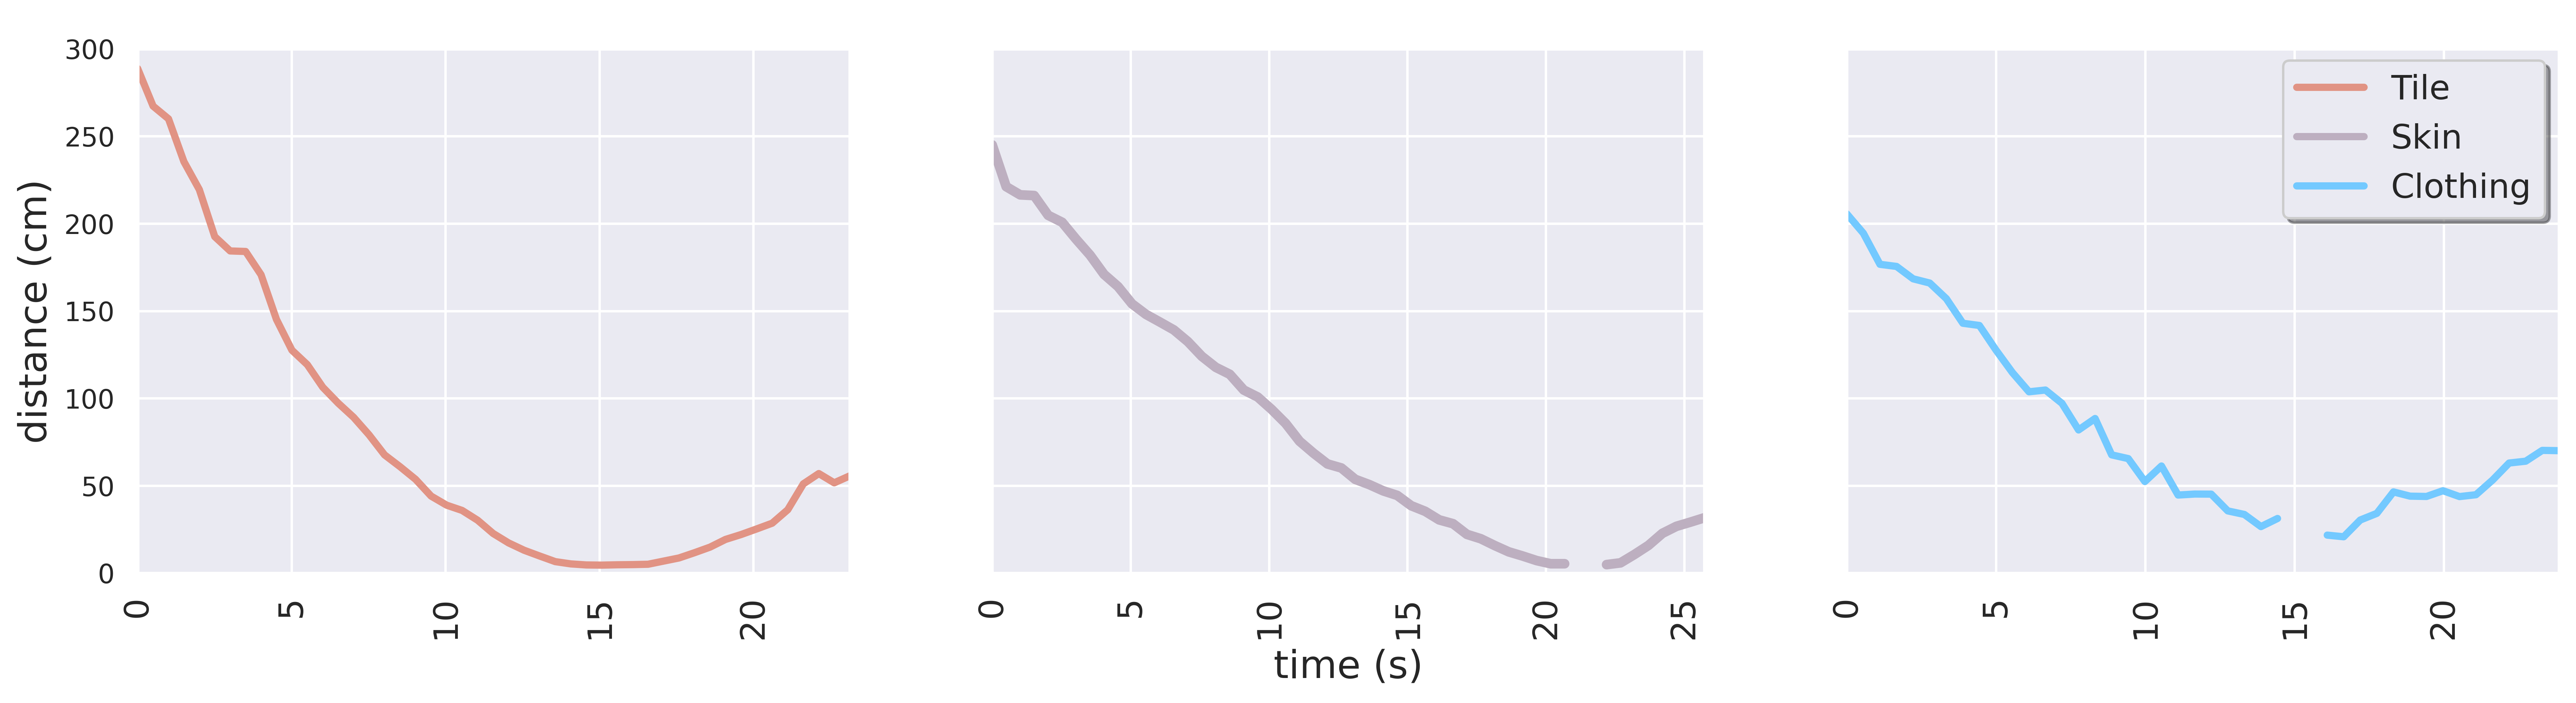
\includegraphics[width=0.85\textwidth,keepaspectratio]{Chapters/Figures/adse_ess/figure5_all_materials_v2.png}
{\caption{Comparison of reflected materials in sample signals. From left to right: ceramic tile, skin from the hand, torso with clothing (on person)}\label{fig:material_comparison}}
\end{figure}
% \vspace*{-40pt}

\subsection{Discussion: Preparing for Public Space}
\label{sec5:discussion}

% Spontaneous and unplanned interactions in space
\subsubsection{New Sociable Space}
% The distancing regulations, realised as a state-enforced requirement have been susceptible of implying social constrains, but is it possible to foresee any sort of positive outcome on the new situation? \citeauthor{mehta_new_2020} point out the overlooked benefits of this \textit{new sociable space} \citeyear{mehta_new_2020}.
On the premise that modern communication technology has shown to facilitate rich social engagements in a remote setting, by which some degree of face-to-face affairs continue to be viewed redundant, even after confinement measures have subsided \citep{cotofan_work_2021}, solutions should also exist to support meaningful discourse from an extendable distance that is suitable for the social environment and individuals involved. Taking shared sound feedback as the core of proxemic mediation, we adopt \citeauthor{mehta_new_2020}'s \citeyear{mehta_new_2020} \textit{new sociable space} concept into our design considerations, this being the capability to capture and hold one's attention from a comfortable distance, encouraging spontaneous encounters with non-acquaintances before confrontation into personal space. Inviting flexibility to traditional proxemic theory, we can call upon Roudposhti's behavioural model that was introduced in Section \ref{sec2_measuring}, demonstrating mannerisms of Indicator and Interest. 
% design consideration
While this desirable social dynamic is provisional to a wide spread of design implications, we put forth the benefit of authorising drop-in and drop-out participation, whereby the formation of a group can be altered at any point to openly accommodate new users. Additionally, this functionality insists upon an agreed focal point of interest that establishes a proxemic cornerstone regardless of the group's composition, continually subject to change. We find this inclusive control structure to be very much customary in the context of interactive installations, such that the initiation of the sound feedback invites new unsuspecting members to engage before even being aware of the artefact's existence \citep{goudarzi_engagement_2016,rostami_bio-sensed_2017}. This function was not explicitly practised in our performance-led study, though we were enlightened through the inclusion of foreign mediation artefacts which became a vital component for exposing extremities of sound output dynamics, shown less prominently when the mask-wearing group were isolated from the external surroundings in scene i. This draws upon the gestural limitations while adhering to a minimum interpersonal distance of 4 feet, absent from any positional cues to prompt collective engagement. 

\subsubsection{Proxemic Sensibility \& Sensitivity}
\label{subsec:sensibility}
% Re socialisation
The \hyperref[sec2:Background]{Literature Review} for this study is comprised of studies that support the vital function that routine social interactions has in organising public spaces and the proceeding benefits that come with this. We also bear in mind the negative view, that undesired social isolation can be detrimental to one's mental condition \citep{evans_social_2019,zorzo_adult_2019,mumtaz_neurobiology_2018}. The pandemic forced prolonged periods of isolation that would ultimately cause a rise in self-reported loneliness \citep{forte_covid-19_2020}, reported to be particularly harmful for those who already experienced anxiety prior to the pandemic period \citep{liang_post-traumatic_2020,brooks_psychological_2020}. Such conditions have been shown to suppress one's tolerance for engagement within intimate proxemic boundaries \citep{layden_loneliness_2018}. We can also include recent findings related to isolation and cognitive function, locating harmful effects on the brain region associated with spatial orientation, learning and memory \citep{rivera_effects_2020,ritchie_cognitive_2020}, which presumably foreshadows a long-term disassociation with in-person social situations. A critical motivation behind our work is to examine what interventions open up a safe intermediate to re-socialisation for individuals who don't yet feel comfortable exposing themselves in public \citep{lupton_coping_2022}, understanding that each person will hold their own preference to personal space.

% Design Consideration
Moving away from a standardised proxemic model, we form an empathetic view around personal space, appreciative of boundaries that are unfixed and individualistic in light of one's past experiences and various other factors that are undisclosed between strangers. Reinforcing Pentland's descriptors assigned previously, this derives from the sentiments that embody Empathy and Interest. In regards to sensory intervention, we articulate the call for proactive awareness as part of the following design considerations, \textit{Proxemic Sensibility} and \textit{Sensitivity}. Sensibility being the altruistic responsibility that ensures safe coordination of bodies, mindful of the surroundings and presence of any individual, paired with Sensitivity, for those to stay receptive to the actions projected by others, with the willingness to alter their paths accordingly. Given the mixed experiences that arose in the presence of external interactive artefacts on stage, these being the flying drone and the unmasked participant group, we speculate on the suitable conditions for effective social signalling through the participatory engagement with sound. Rather than trying to incorporate all of the users simultaneously, we suggest that individualistic control mechanisms can help to elevate one's agency to the surroundings, while the anticipation of regular interchange is necessary to preserve attention. In consequence, we favour the use of structured interruptions by way of turn-taking procedures, whereupon users are compelled to listen to one another, then allocated an sufficient time window in order to react accordingly.

\subsubsection{Constrained Complexity}
\label{subsec:discussion_complexity}

This work fits into the domain of proxemic interaction strategies, asserting novelty in the non-categorisation of physical distances. The early phases of experimentation lead us to try complex, non-linear sound-distance mapping strategies without the anticipation of hindered usability. However, we were enlightened early into prototyping that such sophisticated mapping strategies are only intuitive on the presumption that users are sufficiently acquainted with the apparatus and expected results, reiterating discussions around the virtuosity of musical instruments within the NIME research community \citep{wu_supporting_2017}. We first insisted on more abstract mappings, layering sound elements each influenced by multiple users simultaneously; this approach was designed to provoke collective actions and consequentially, for the group to act upon the movement patterns that made the most sense to them. From this composite sound feedback strategy, however, emerged a great deal of confusion from new users, leaving them with a feeling of disempowerment. We found this ambitious setup expected far too much knowledge from new users, made clear during testing, where participants would express their frustrations with the system's behaviour while not understanding how their individual actions influence what they were hearing. At a minimum, they would want to walk closer or farther from someone and hear an instantaneous reaction. We were able to recover the user's association to the sound feedback when resorting to a linear distance to amplitude mapping according to the smallest distance detected, allocating control to only one individual at a time in favour of being perceived more receptive. Though in many cases, the irregular substitutions would cause excessive shifts in volume, disrupting the continuity of the controlling gesture. In particular, when incorporating external objects and additional users onto the stage, we find more instances of abrupt sound bursts, depicted by the intermittent gaps in the audio recording, as shown in Figure \ref{fig:interuptions-spectograpm}. 

% In Section \ref{subsec:soundInteraction}, we praise the eloquent control that groups of trained musicians can offer to digital music systems, a realm that has undeniably come as a major inspiration to this work. In this case, however, the orchestration became more inclusive as we transitioned away from trying to resemble such collaborative systems presented in music-orientated fields such as NIME \citep{poupyrev2001new}, and instead focused on sound mechanisms that new users could immediately take control over, advocating for a shallow learning curve. 
While working in this semi-controlled setting, we benefited from the user's past experiences using digital musical instruments. However, when gearing towards a public space intervention, the importance of bridging with broader audiences would become most salient, to engage those unfamiliar with the system and each other, as described in Section \ref{sec:public_adaptation}. Such a pursuit calls for an accessible means of individual control that also encourages collaboration amongst strangers. Here, we advocate for a turn-taking framework that operates on a fixed time interval. This conveniently aligns with the step sequencer metaphor proposed in \citeauthor{bengler_designing_2013}'s \citeyear{bengler_designing_2013} work with non-musicians, studying how a constrained control paradigm can improve engagement with the general public. To build upon these considerations, we prescribe the function of sequencing for distributed control and attention in group interaction, maintaining the usability of single-user mappings whilst emphasising the quality of observing the other.

\subsubsection{Precautions for Public Inclusion}
% \label{subsec:safety}

The change in pandemic circumstances that happened during the research timeline meant that only a maximum of 4 participants were authorised to use the wearable at any one time, dismissing any substitution of users between daily intervals. This compromised the conditions for open public inclusion while the measures gradually became stricter, bringing serious doubts in justifying any sort of artistic action that persisted in congregating different social bubbles. In these circumstances, we were confronted with the fragility of the sensory components embedded onto the mask, while the constantly shifting directions meant that misreadings were highly probable. More often than not, assistance was required from the workshop coordinator to secure the wearable around the user's head; this would unfavourably call for physical contact near the mouth, posing an additional risk of viral transmission. That considered, a harmful misfortune such as this would have been far more problematic if widespread into public hands.

The deferred extremity of the situation was only realised around one month later, as these measures would come forth as a final phase of provisionary measures before the nation was required to fall under a compulsory confinement period (i.e. lockdown). On these terms, the study was committed to the a public space intervention with elevated awareness on safety and robustness, particularly in regards to the exchange of wearable components between alternating user groups. 

At the time of reorganising the study, this absence of open public participation was deemed somewhat a pitiful solution, albeit one that avoids abandoning the in-person field study indefinitely. But in hindsight, we realise these intermediate steps were absolutely necessary before a system like this could be made accessible to the public, ensuring usability and safety to a minimum standard. These preparations were made evident in the adaption process for public space, presented in Section \ref{sec:public_adaptation}. This mentality of turning restrictions into opportunities for precaution is highly acclaimed in the discussions drawn out from \cite{howell_life-affirming_2019}. This work rationalises the function of private space experimentation which would merit design guidelines for public interventions, detailing concerns around safety that would omit the likelihood of welcoming fruitful interactions between strangers. Nonetheless, in lack of public exposure, arises the opportunity to grasp deeper insights from the user group. We factor this progression into our design considerations, insisting that new systems intended for public use should first be evaluated in a low-risk environment for a substantial period of time, taking opportunities to carry out data collection and open-ended experimentation.

\section{The Case for Public Interventions During a Pandemic}
\label{sec:public_adaptation}

To wrap up what was learned during the first phase of experimentation and preliminary study, we introduce an adaptation for a proxemic-based sound intervention designed for open urban spaces, materialised some months later, while the most prominent pandemic regulations were already lifted. This demonstration was set out to provoke collaborative engagement through sound, similar to what was observed during the closed user-study, but in contrast, situated in the public space format that was envisioned since the project's original ideation. The system was installed for three full days in a touristic square close to the city centre, completely open to any passing members of the general public. Participants were expected to make use of the system independently, offered only a set of essential instructions that were made accessible online through a mobile web application. Enlightened by our design considerations, we detail an alternative method for distance-to-sound interaction and assess to what extent, this intervention was capable of preserving the qualities of interaction that were preconceived in the discussion. Here, we evaluate the following strategies: drop-in and out participation, structured interruptions, and sequencing.

\subsubsection{Instrumentation and Physical Arrangement}

The public sensing environment brought many challenges to the system's physical orchestration. The major conditions here may be subject to the installation sustaining itself outdoors, and the considerations in order for it to operate independently without facilitators. We were also intrigued to experiment more deeply into proxemic affordances shaped by the surrounding environment and non-human objects. First off, we reconsidered the mask-worn device to grant user independence, improve safety against viral transmission and refrain from dealing with inaccuracies. As an alternative, four proximity sensors were secured around the lower branches of a tree, pointing slightly downward to establish a path from the tree's crown to a seating area set up 16 feet away from the base of the tree. 

Along with each sensor hangs a brightly coloured ribbon from the branch, representing the origin of the individual paths, indicating the course for users to walk under, as annotated in Figure \ref{fig:installation_sensor_setup}. The extent of the projected sensing area was bounded by the maximum sensing distance, capped at 12 feet to maintain reliability. Granted that the sensor's performance is dependable on the ambient temperature and humidity, we noticed the detectable range varied more throughout the day than when we were working indoors. The air temperatures would fluctuate from 9-20 \celsius  daily, with generally worsening detection rates during the night. 

\begin{figure}[!h]
\centering
\includegraphics[width=\textwidth,keepaspectratio]{Chapters/Figures/adse_ess/sensing_area_merged_w_diagram_optimized.png}
{
\caption{Public installation using four proximity sensors placed inside foliage with hanging ribbon. Sensors are physically separated by sensing trajectories, identified by colour.
}
\label{fig:installation_sensor_setup}
}
\vspace*{-20pt}
\end{figure}

\subsection{Spatially Distributed Sound Output}

It was in our prime interest that the intervention would preserve the inherent tranquillity of the pedestrian area. To avoid any unnecessary disruption, we insisted that the installation would not exert any sound until participants were willing to engage with the system. We speculated upon a feasible solution by which the public could initiate the sensing mechanism and listen to the installation from their mobile phone. A web app was developed using the \textit{Soundworks} web framework by \citeauthor{matuszewski_interaction_2019}. Upon loading the app, participants are prompted to select one of four colours each allocated to one of the sensor placements, determinant of a walking path (Figure \ref{fig:installation_instructions}). The individual sensor measurements are broadcast to each of the mobile phones connected to the current session, activating new notes when someone is detected in the space and continues to do so while the participant moves within the measurable path.

The occlusion distance from each sensor was recorded in consecutive order, cycling through the complete batch every quarter-of-a-second. The distances are converted into MIDI notes on a single octave chromatic scale, allowing 12 possibilities spread out between 30cm intervals, rising in pitch as the distance measured from the sensor increases. When a user is detected, the app arpeggiates through the incoming notes every cycle. As one note is released, a new note is triggered from the neighbouring user according to their detected distance. Each note is emitted from the mobile device that's assigned to the coloured sensing path, accumulating into short loops that are continuously recorded and echoed in ongoing circulation.

\begin{figure}[!h]
\centering
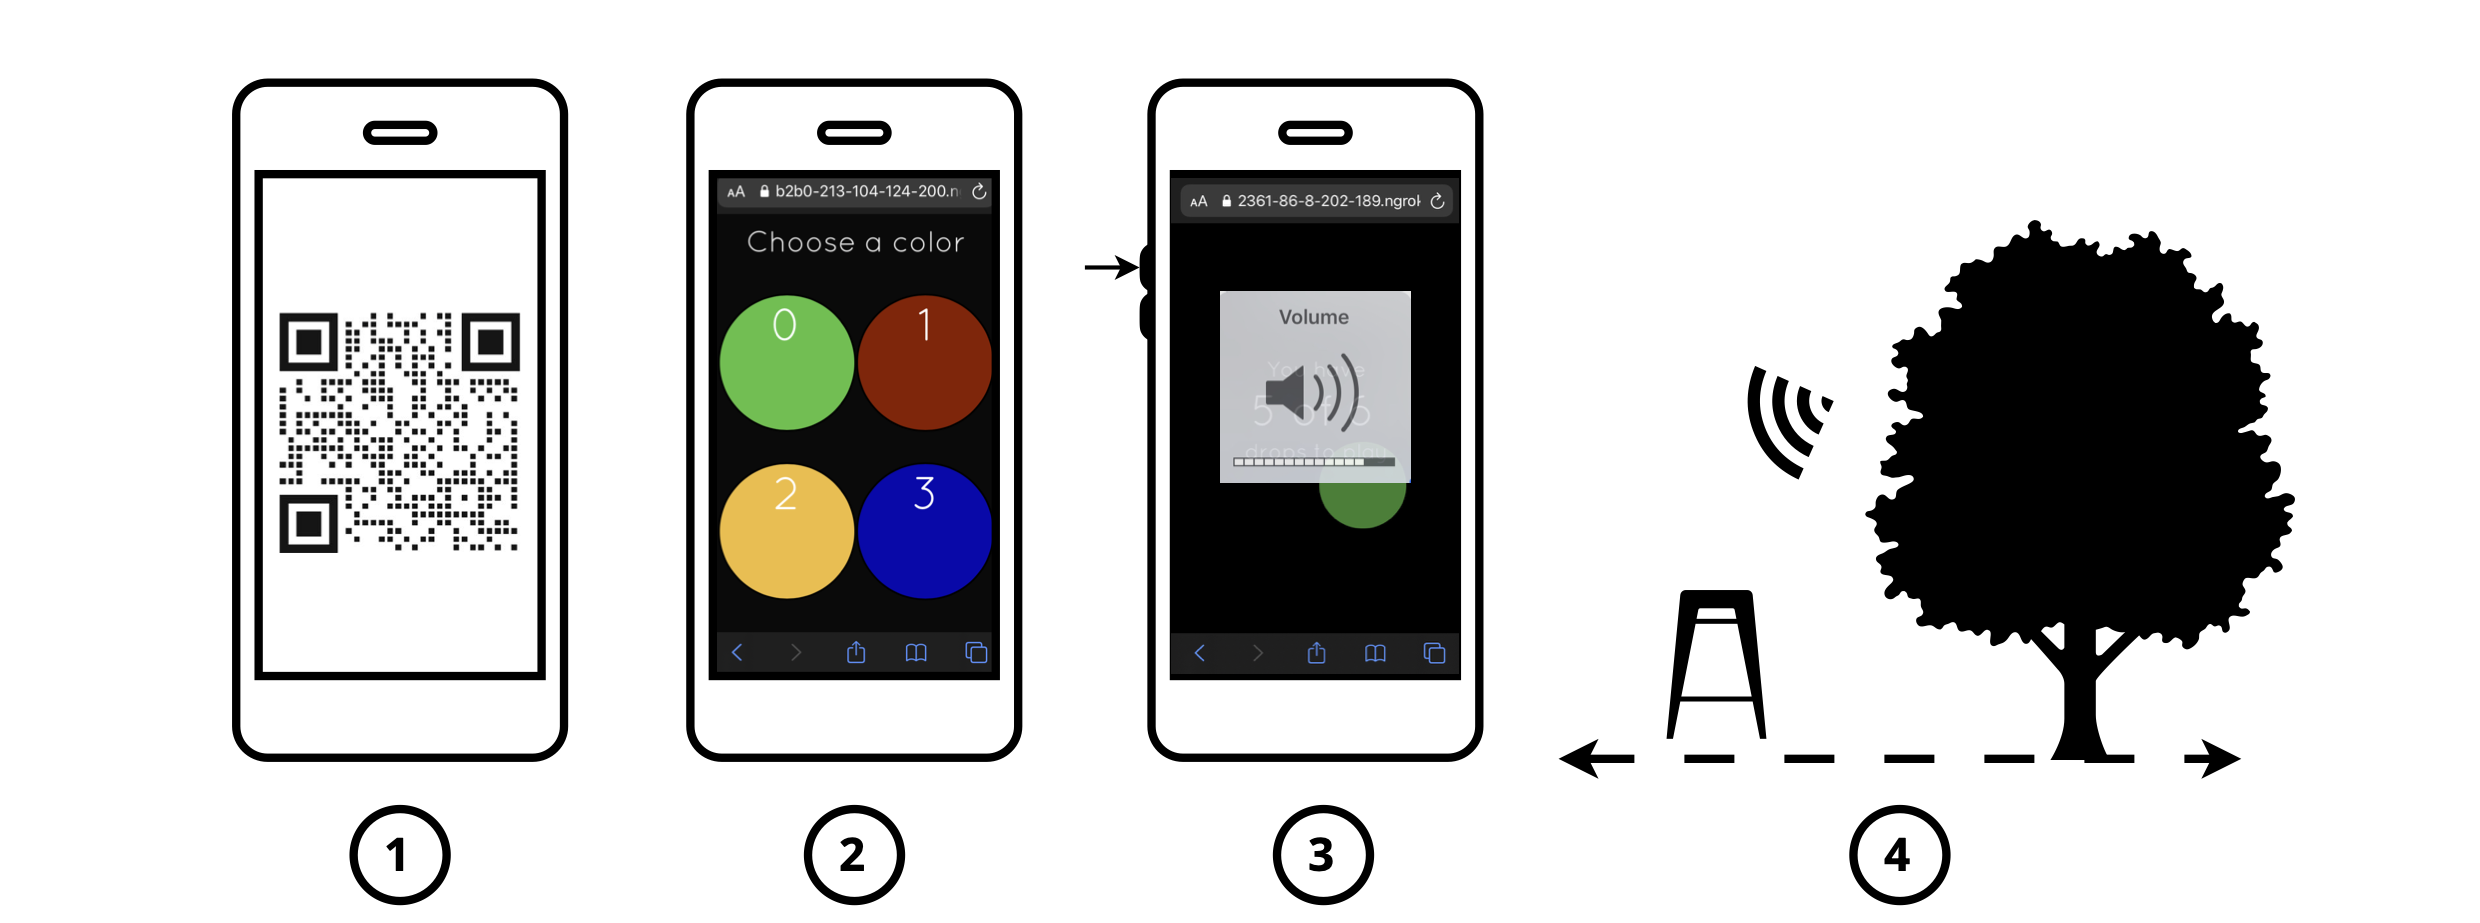
\includegraphics[width=0.9\textwidth,keepaspectratio]{Chapters/Figures/adse_ess/ADSE-WP-INSTRUCTIONS.png}
{
\caption{User instructions for installation: (1) Access QR code, (2) load the app and select a colour, (3) increase the device volume, and (4) walk towards the chosen colour to initiate sound}
\label{fig:installation_instructions}
}
\end{figure}

\subsubsection{From Lab to City, Transferable Experiential Qualities}
\label{sec:fromLabToCity}

Over the course of the installation period, we made notes of third-person observational accounts, similar to the rehearsal sessions and performance described prior to this. In particular, we give close attention to moments of group engagement that resonated with the spatial qualities examined previously, thus disclosing the experiences that were transferable from the wearable device to the public space adaptation. This numerical evaluation here does not intend to go as in-depth as the initial study, instead, this closing segment can be considered as a technical primer to fortify our design considerations for future research set in public space environments.

Advancing upon \textit{proxemic sensibility} and turn-taking qualities, we found the mobile distributed sequencer fostered a certain degree of mutual agency, in that participants would invite their peers to join them and instinctively feel be inclined to listen to one another. While exploring different spatial configurations, users would continuously experience new melodic loops with each note coming from separate directions according to the user's position. The separation of the mobile speakers in of itself provided an additional modality to the acoustic quality of the soundscape, formed by the relationship between perceived intensity and distance. For the most part, however, users were staring directly at their mobile phone during interaction, with their bodies constantly turned towards the sensing apparatus standing parallel to each other, majorly discouraging prospects for mutual acknowledgement through eye contact.

From an observational standpoint, it was not possible to discern synchronous movement patterns inspired by the installation, or any definitive collective movement traits for that matter. Compared to the first case study, resourced with a large stage, the spatial exploration was far more limited here, restricted only to a linear sensing area, revolving around one focal point. Users would insist on staying idle, waiting for the sound to loop for a while, perhaps experimenting with walking forwards or backwards a few steps to trigger new notes. This coincides with the outcomes that presented themselves in Scene ii (Section \ref{sec:structure}) in the way that, when the directional influence of the sensors is displaced from the body and onto the surroundings, users show more infatuation with their own movements over anyone else's. With the ambition to cater for a \textit{new sociable space}, the non-wearable arrangement combined with the drop-in and out functionality of the app was assumed to incentivise a flexible interchange of users, inclined to welcome those non-acquainted into the space. That said, we did not observe any instances of strangers simultaneously engaging at the same time, only those already affiliated, supposedly conditioned to the tensions when asserting oneself into a predetermined social clique. 

In this instance, we wish to examine how well the intervention harmonises with the everyday operation of the space, blending with naturally occurring social exchanges, staying respectful to those not actively participating. We found from a sample of 10 individuals and groups passing by during a weekday afternoon, 7 of 10 would continue walking, 3 would feel captivated to read the information board with 1 going as far as entering themselves into the application, and start to engage with the sound feedback. During the weekend period, the installation would be stationed along the route of a few public walking tours, serving as an amusing artefact to intrigued bystanders, without pulling enough attention for anyone to abandon their personal schedule. In the evening, we observed a spontaneous social gathering take place in the square comprised of 15 or more people mingling beside the installation area. In this instance, small groups would approach the installation and briefly engage in a new session, triggering just a few notes before returning back to rejoin the social event. Accepting the severe limitations in retaining interest from new users, these impulsive engagements showcase a strong starting point for public inclusion, by which the artefact successfully captures the attention of broader audiences enough for voluntary initiation. This can partly be owed to our preparation stages, pleading for \textit{constrained complexity} to minimise the learning curve.

\subsubsection{Limitations of Public Space Adaptations}

In this supplementary case study, we were granted the opportunity to confront the challenges of proxemic sensing in public space; this exposed a number of external factors that were less problematic in semi-controlled conditions. We discuss design decisions that were influenced by environmental changes, technical durability and usability, contributing to pervasiveness and inclusion. The non-wearable solution was less susceptible to errors, but at the expense of a confined sensing area. The linear note-based interaction combined with the fixed placement of the sensor improved the system's usability when it was made openly accessible to a public audience. With that said, we believe this approach minimised the user's resilience to unexpected outcomes, made apparent the moment that sound would stop playing, user's would immediately lose interest and move on to proceed with the rest of their day. In lack of a firm recommendation here, these outcomes continue to linger onto the feasibility of engaging unskilled users with novel interactive music systems \citep{holland_musical_2019}, only to be exaggerated in a pervasive setting where prolonged participation is nonobligatory. In its wearable form, the original orchestration was purposed specifically to capture group dynamics by way of geometric and temporal relationships. But here, we discern that the users were not highly aware of the movements happening around them. This persuasion may be accredited to the animations that are triggered concurrently within the application window, for which the extra stimulation has an overriding effect on mutual engagement, as is inferred by \citeauthor{bryan-kinns_mutual_2013}'s \citeyear{bryan-kinns_mutual_2013} study. Coinciding with the issues we faced when introducing additional visual elements, the authors ultimately caution against an excessive exposure to non-essential information in order to maintain attention in a collaborative interaction setting.

% \vspace*{-5pt}

% \vspace*{-12pt}
\subsection{Conclusion}

This study reflects upon the common attitudes associated with interpersonal distancing and social connection during the most critical moments of pandemia. We speculate upon a spatially-informed intervention to be deployed as part of a performance; this incentivised the design of a sensory face-mask, coupled with a system for sound interaction. This wearable orchestration was trailed over a series of workshop sessions, inviting participatory feedback used to refine the physical design and mapping strategies in anticipation to be presented in a live performance setting. Reflecting upon observational notes and data analysis, we construct design considerations that respond to the pivotal challenges surrounding safe, inclusive re-socialisation in public and in theory, what spatially sensitive systems can offer to overcome such issues. This ultimately calls for an individualistic understanding of proxemic boundaries, giving agency to neighbouring bodies through sequential control, adaptable participation and constrained complexity strategies. We frame our findings in a broader perspective on sensory interventions that are not solely relevant to pandemic measures, generating critical reflections that later inform future developments as we appropriate the system towards urban sensing environments, proving transferable qualities amidst persisting limitations when subjected to the general public. We outline the standout progressions between the two sensing mechanisms, one situated directly onto the body, the other installed into the surroundings, proving transferable qualities amidst persisting limitations when subjected to the general public. For future work, we foresee a benefit of incorporating a hybrid system comprised of wearable and environmental sensors, suitable for large open spaces in the confidence of robust operation.

% \begin{Backmatter}
% \label{sec:appendix}
% \appendix

% \paragraph{Supplementary material} \label{SupplementaryMaterial}
% % To view supplementary material for this article, please visit \url{http://dx.doi.org/10.1017/wtc.2019.116}.

% \begin{itemize}
% \item Adapted firmware and circuitry schematic: \url{https://gitlab.com/wprimett/bitalino-riot-hc-sr04/-/tree/master}
% \item Adjustable mask strap and microcontroller enclosure:
% \url{https://www.tinkercad.com/things/j67Mtut3IZk}
% \item Sensor housing and nasal attachment (back panel):
% \url{https://www.tinkercad.com/things/aDBQI4QbteS}
% \item Sensor housing and nasal attachment (front panel):
% \url{https://www.tinkercad.com/things/cLQBlFGjHOL}
% \item Rehearsal Video Extract:
% \url{https://vimeo.com/651050353/6c20506f98}
% \item Performance Video Extract:
% \url{https://vimeo.com/653807254/6c72e1ce28}
% \item Sound Installation Video:
% \url{https://vimeo.com/703689060/71faea44dc}
% \item Acceleration Data Graph:
% \textit{in submission}
% \end{itemize}

